% Version 0; preprint format; Written by SH
% Version 1; emulateapj format; Edited by SH and AL

%\documentclass[twocolumn]{aastex6}
\documentclass{emulateapj}

% Packages
%\usepackage{emulateapj5}
\usepackage{apjfonts}
\usepackage{amssymb, amsmath}
\usepackage{graphicx}
\usepackage{CJK}
\usepackage{natbib}
\usepackage{hyperref}
\usepackage{float}
\usepackage[usenames, dvipsnames]{color}

% Package Settings
\bibliographystyle{apj}
\hypersetup{colorlinks=true,
            citecolor=cyan,
            linkcolor=cyan,
            filecolor=magenta,      
            urlcolor=cyan}
\urlstyle{same}

% Figure extention
\DeclareGraphicsExtensions{.pdf,.png,.jpg}
\input psfig.tex

%%%%%%%%%%%%: User Defined Commands %%%%%%%%%%%%

% Song Huang's definition 
\def\arcsec{{\prime\prime}}
\def\arcmin{{\prime}}
\def\degree{{\circ}}
\def\h{\hskip -3 mm}
\def\aa{{A\&A}}
\def\aas{{ A\&AS}}
\def\aj{{AJ}}
\def\al{$\alpha$}
\def\bet{$\beta$}
\def\amin{$^\prime$}
\def\annrev{{ARA\&A}}
\def\apj{{ApJ}}
\def\apjs{{ApJS}}
\def\asec{$^{\prime\prime}$}
\def\deg{$^{\circ}$}
\def\ddeg{{\rlap.}$^{\circ}$}
\def\dsec{{\rlap.}$^{\prime\prime}$}
\def\cc{cm$^{-3}$}
\def\flamb{erg s$^{-1}$ cm$^{-2}$ \AA$^{-1}$}
\def\flux{erg s$^{-1}$ cm$^{-2}$}
\def\fnu{erg s$^{-1}$ cm$^{-2}$ Hz$^{-1}$}
\def\hst{{\textit{HST}}}
\def\kms{km s$^{-1}$}
\def\lamb{$\lambda$}
\def\lax{{$\mathrel{\hbox{\rlap{\hbox{\lower4pt\hbox{$\sim$}}}\hbox{$<$}}}$}}
\def\gax{{$\mathrel{\hbox{\rlap{\hbox{\lower4pt\hbox{$\sim$}}}\hbox{$>$}}}$}}
\def\simlt{\lower.5ex\hbox{$\; \buildrel < \over \sim \;$}}
\def\simgt{\lower.5ex\hbox{$\; \buildrel > \over \sim \;$}}
\def\micron{{$\mu$m}}
\def\mnras{{MNRAS}}
\def\nat{{Nature}}
\def\pasp{{PASP}}
\def\perang{\AA$^{-1}$}
\def\peryr{yr$^{-1}$}
\def\reference{\noindent\pp}
\def\refindent{\par\noindent\parskip=2pt\hangindent=3pc\hangafter=1 }
\def\sb{mag~arcsec$^{-2}$}
\def\lsun{$L_\odot$}
\def\msun{$M_\odot$}
\def\sigs{$\sigma_*$}
\newcommand{\lt}{<}
\newcommand{\gt}{>}

\def\etal{{\ et al.~}}
\def\galfit{{\tt GALFIT}}
\def\ser{{S\'{e}rsic\ }}
\def\redm{\texttt{redMaPPer}}
\def\cmodel{\texttt{cModel}}
% Samples
\def\rbcg{\texttt{cenHighMh}}
\def\nbcg{\texttt{cenLowMh}}
\def\redbcg{{$\lambda \ge 30$}}
\def\nonbcg{{$\lambda < 20$}}
% Mass related 
\def\mstar{{$M_{\star}$}}
\def\mhalo{{$M_{\mathrm{halo}}$}}
\def\logms{{$\log (M_{\star}/M_{\odot})$}}
\def\logmh{{$\log (M_{\mathrm{Halo}}/M_{\odot})$}}

\def\minn{{$M_{\star,10\mathrm{kpc}}$}}
\def\meff{{$M_{\star,15\mathrm{kpc}}$}} 
\def\mtot{{$M_{\star,100\mathrm{kpc}}$}}
\def\mout{{$M_{\star,150\mathrm{kpc}}$}}
\def\mmax{{$M_{\star,\mathrm{Max}}$}}
\def\mgama{{$M_{\star,\mathrm{GAMA}}$}}
\def\mcmodel{{$M_{\star,\mathrm{cModel}}$}}

\def\logminn{{$\log (M_{\star,10\mathrm{kpc}}/M_{\odot})$}}
\def\logmtot{{$\log (M_{\star,100\mathrm{kpc}}/M_{\odot})$}}
\def\logmout{{$\log (M_{\star,150\mathrm{kpc}}/M_{\odot})$}}
\def\logmmax{{$\log (M_{\star,\mathrm{Max}}/M_{\odot})$}}
\def\logmgama{{$\log (M_{\star,mathrm{GAMA}}/M_{\odot})$}}
\def\logmcmodel{{$\log (M_{\star,mathrm{cModel}}/M_{\odot})$}}

\def\m2l{{$M_{\star}/L_{\star}$}}
\def\mden{{$\mu_{\star}$}}


% Commenting:
\newcommand{\xxx}[1]{\textcolor{red}{\textbf{XXX}}}
\newcommand{\todo}[1]{\textcolor{red}{\textbf{TODO:~#1}}}
\newcommand{\plan}[1]{\textcolor{cyan}{#1}}
\newcommand{\addref}{{\textcolor{red}{REF}}}
\newcommand{\note}[2]{\textcolor{blue}{\textbf{[Comment (#1): #2]}}}
\newcommand{\song}[1]{\textcolor{magenta}{\textbf{[Song: #1]}}}
\newcommand{\alexie}[1]{\textcolor{blue}{\textbf{[Alexie: #1]}}}
\newcommand{\kevin}[1]{\textcolor{green}{\textbf{[Kevin: #1]}}}
\newcommand{\update}[1]{\textcolor{Bittersweet}{#1}}

%%%%%%%%%%%%: Header and Version %%%%%%%%%%%%

\shorttitle{ENVIRONMENT DEPENDENCE OF MASS-SIZE RELATION}
\shortauthors{HUANG ET AL.}
\slugcomment{Draft version 0}

\begin{document}

\begin{CJK*}{UTF8}{gbsn}

%%%%%%%%%%%%: Title and Affiliations %%%%%%%%%%%%

%\title{The Environment and Structure of Massive Central Galaxies
%       using the Subaru Hyper Suprime-Cam Survey}

\title{First Detection of the Environmental Dependence of the Structures of Massive Galaxies }


\author{Song Huang (黄崧)\altaffilmark{1}, 
        HSC collaboration\altaffilmark{1}}   
%        \author{Song Huang (黄崧)\altaffilmark{1} 
%        Alexie Leauthaud\altaffilmark{1}, 
%        Kevin Bundy\altaffilmark{1},
%        Michael Strauss\altaffilmark{2},
%        Yen-Ting Lin\altaffilmark{3},
%        Rachel Mandelbaum\altaffilmark{4}
%        }
        
        
\email{song.huang@ipmu.jp}

\date{}                                          

\altaffiltext{1}{Kavli Institute for the Physics and Mathematics of the 
    Universe, The University of Tokyo Institutes for Advanced Study, 
    the University of Tokyo (Kavli IPMU, WPI), Kashiwa 277--8583, Japan}
%\altaffiltext{2}{Princeton University Observatory, 
%    Peyton Hall, Princeton, NJ 08544, USA}
%\altaffiltext{3}{Institute of Astronomy and Astrophysics, Academia Sinica, 
%    P.O.~Box 23--141, Taipei 10617, Taiwan}
%\altaffiltext{4}{Carnegie-Mellon University \todo{correct affiliation here}}

%%%%%%%%%%%%: Abstract and Keywords %%%%%%%%%%%%

\begin{abstract}

    Although the environmental dependence of structures for massive central 
    galaxies is predicted by the promising hierarchical assembly model, 
    observations at low redshift seem to find no convincing evidence for that. 
    With the help of deep $i$-band images of a large sample of massive central 
    galaxies at $0.3 < z < 0.5$ from the Subaru Hyper Suprime-Cam (HSC) survey, 
    we map their stellar mass distributions out to radius larger than $100$ kpc, 
    and discover subtle, but systematic and robust structural differences that 
    depend on halo mass. 
    At fixed stellar mass within 100 kpc, the massive central galaxies in more 
    massive ($M_{200m} > 1.6\times 10^{14} M_{\odot}$) halos have a 
    slightly flattened inner profile within $\sim 15$-$20$ kpc, and a more prominent 
    outer envelope compared to ones in less massive 
    ($M_{200m}>8.7\times 10^{13} M_{\odot}$) halos.
    For centrals with $M_{\star} > 10^{11.5} M_{\odot}$, the ones in more massive 
    halos show very significant excess of mass in the outskirt when the two samples 
    are matched using proxies of mass assembled at $z > 1$. 
    Such differences are broadly consistent with richer recent merging history 
    for more massive halos. 
    We suggest that the relation between total stellar mass and mass within inner 5 
    or 10 kpc is potentially interesting for diagnosing the role played by host halo 
    in shaping the structures of massive central galaxies. 
    These results also highlight the importance of deep photometry and the usage of 
    detailed structural information in the study of the assembly history of galaxies. 

\end{abstract}
\keywords{galaxies: elliptical and lenticular, cD --- galaxies: formation --- 
          galaxies: photometry --- galaxies: structure --- galaxies: surveys}

\maketitle

%%%%%%%%%%%%: Main Text %%%%%%%%%%%%

%% ------------------------------------------------------------------------------------ %% 
    \begin{figure*}[t!]
        \centering 
        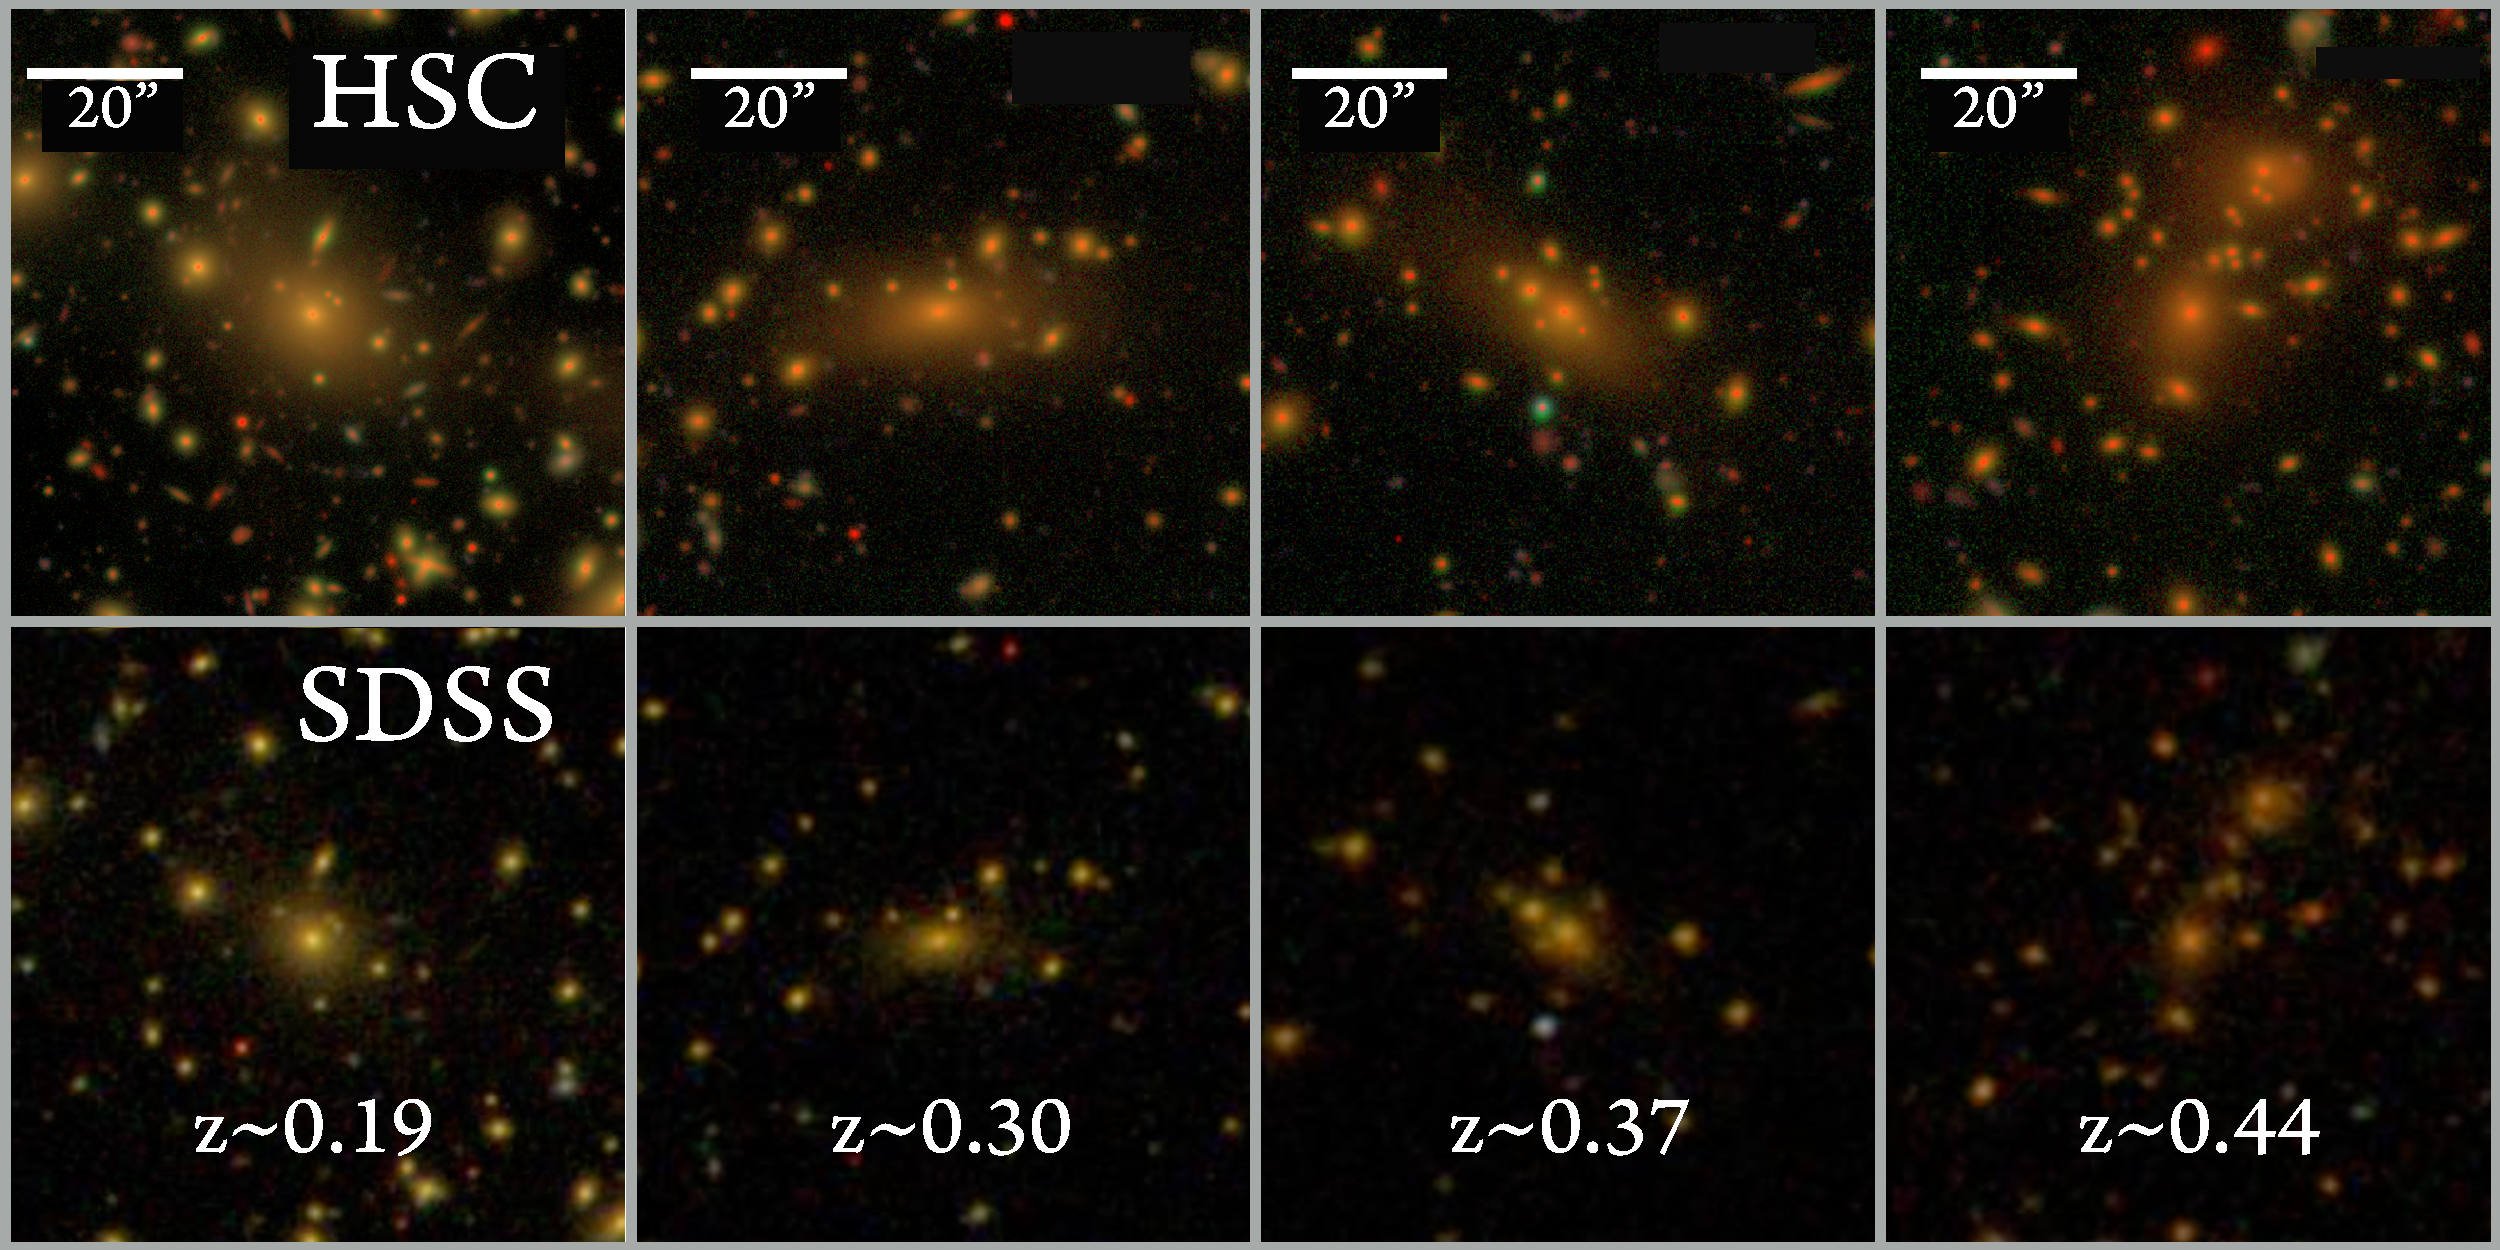
\includegraphics[width=\textwidth]{fig/redbcg_sdss_compare}
        \caption{A comparison between the imaging quality of SDSS and HSC Wide for a sample 
        	of nearby massive elliptical galaxies at $0.2 < z < 0.5$.  
            These images are generated using $gri$ band images with an arcsinh stretch 
            \citep{Lupton2004}. 
            The HSC Wide layer is $3.0$-$4.0$ magnitudes deeper than SDSS which is 
            critical in order to map the outskirts of ETGs out to large radii.}
        \label{fig:sdss_compare}
    \end{figure*}
%% ------------------------------------------------------------------------------------ %% 

%% ------------------------------------------------------------------------------------ %% 
  \begin{figure*}[t!]
      \centering 
      \includegraphics[width=\textwidth]{fig/redbcg_m100_m10_compare}
      \caption{Three-color images for a subsample of massive galaxies at similar redshift
      		($\sim 0.4$), and with similar \mstar{} inside inner 10 kpc (indicated by the 
            dash-line cicle on top-left figure; 
            $11.2<\log (M_{\star,10\ \mathrm{kpc}}/M_{\odot})<11.3$). 
            However, they span quite a large range in \mstar{} within 100 kpc 
            (highlighted by the solid bar on the top-left figure). 
            From top-left to bottom-right, their \mtot{} increases from 
            $10^{11.2} M_{\odot}$ to $10^{11.7} M_{\odot}$.
            The three galaxies from \rbcg{} sample are highlighted via red frames.
            }
      \label{fig:m100_m10_color}
  \end{figure*}
%% ------------------------------------------------------------------------------------ %% 

%% ------------------------------------------------------------------------------------ %% 
\section{Introduction}
    \label{sec:intro}
    
    \plan{Scientific Background}
    \begin{itemize}
        \item \plan{Massive galaxies are important cosmic probe and unique labs to study 
            galaxy evolution.} 
        \item \plan{Briefly explain why massive early-type galaxies are important through 
            the difficulties of stellar-halo mass relation and stellar mass function at 
            the high-mass end.}
        \item \plan{Brief summary of the current understanding of their cosmic assembly 
            history.}
        \item \plan{Explain why we should care about the environment, and why we expect to 
            see some environmental dependence in the structure and other properties of
            massive galaxies.}
        \item \plan{Brief review of the current observations.  It is still not clear 
            whether there is a clear environmental dependence.}
    \end{itemize}

    \plan{Observational difficulties (a.k.a Why we need HSC)}
    \begin{itemize}
        \item \plan{Explain why it is important to study the mass distribution of 
            massive galaxies out to large physical radius; and, given their unique light 
            profiles, why it is more difficult to study them compared to late-type 
            galaxies.}
        \item \plan{Very brief summary of past observational efforts, and why they are not 
            good enough (Not enough number of really massive galaxy; Shallow images; 
            Background subtraction issue; and stacking analysis can be dangerous as while)}
    \end{itemize}
    
    \plan{Basic idea of this work}
    \begin{itemize}
        \item \plan{Here we take advantages of the ambitious Hyper-Suprime camera 
            survey\ldots}
    \end{itemize}
        
    \update{Here, we take advantage of the excellent image quality of the HSC survey, and 
    investigate the potential environmental dependence of structure for massive galaxies 
    vial comparing the surface \mstar{} density profiles and structural scaling relations 
    between massive central galaxies in different environments. 
    As shown in Fig.\ref{fig:sdss_compare}, the HSC $i$-band images are typically 3-4 
    magnitude deeper than SDSS ones, and have much better seeing condition 
    (median FWHM$\sim 0.6^{\arcsec}$), hence they are perfect for mapping the \mstar{}
    distributions of massive galaxies out to very large radius. 
    With the help of a cluster catalog, we select a large sample of massive central 
    galaxies in halos that are more or less massive than \logmh{}$\sim 14.0$ at 
    $0.3 < z < 0.5$ from the available $\sim 100$ square degree of HSC data.}
    
    \update{Due to the difficulty in appropriately modeling the \mstar{} distributions of 
    massive galaxies out to their very outskirts, we focus on \mstar{} within two different 
    physical apertures in this work:}
    
    \begin{itemize}
        \item \update{\mstar{} within 10 kpc, \minn{}: according to the ``two-phase'' 
            scenario, the ``in-situ'' star-formation quickly built up the inner, dense 
            core of massive ETGs.  
            Based on recent observations and simulations (e.g.~\citealt{vanDokkum2010}; 
            \citealt{RodriguezGomez2016}), the in-situ 
            component distributes mostly within the effect radius ($R_{\mathrm{e}}$, 
            or 5-10 kpc) in massive galaxies.  
            Here we use \minn{} as a proxy of the \mstar{} formed in the ``in-situ''
            phase.  Although it is an empirical choice, the detailed comparison of 
            the stellar mass surface density (\mden{}) profiles later suggests it indeed 
            helps reveal interesting environmental dependence.  
            Under the adopted cosmology, $1.0^{\arcsec}$ in radius equals 4.4 and 6.1 kpc 
            at redshift 0.3 and 0.5.  
            We can reliably measure \minn{} without being bothered by smearing effect
            of seeing.}
        \item \update{\mstar{} within 100 kpc, \mtot{}: for massive galaxies in this work, 
            100 kpc aperture reaches to 5-10 $\times R_{\mathrm{e}}$ and very low 
            \mden{} region, hence can be treated as proxy of the ``total'' \mstar{}. 
            Limited by the accuracy of background subtraction, the \mden{} profile 
            of outer region can not be reliably recovered for massive galaxies across 
            our redshift range. 
            Although not perfect, \mtot{} is still a much better tracer of total 
            \mstar{} than the model-dependent ones using shallower images.}
    \end{itemize}
    
    \update{Massive central galaxies in this work show an intriguing diversity on the 
    plane defined by these two metrics.  
    We preview this using Fig.\ref{fig:m100_m10_color}, which shows a subsample of 
    massive galaxies at $z\sim 0.4$ that share very similar value of \minn{}, but show 
    a large range of outer structures. 
    Assuming galaxies at the same \minn{} have similar amount stars in the in-situ 
    component, it is of great interest to investigate the relation between their 
    environments and outer envelopes that are assembled at later time. 
    It is worth noting that, although a circular aperture is shown on 
    Fig.\ref{fig:m100_m10_color}, we always use elliptical apertures that follow the 
    average isophotal shape for photometry in this work.}
    And, within our choices of redshift and \mstar{} ranges, we can safely ignore 
    significant mass growth and structural evolution 
    (no star formation, lower merger rate \etal~e.g.\ \citealt{Bellstedt2016},
    \citealt{Inagaki2015}; but also see \citealt{Bai2014}) 
    with our redshift and \mstar{} ranges. 

    The paper is organized as follows. Section\ref{sec:data} gives a brief overview of 
    the HSC observation and data reduction, along with the summary of the data selection
    processes.  
    Then, we will explain the procedures for extracting 1-D surface brightness profiles 
    (Section \ref{sec:ellipse}) and estimating stellar mass (Section \ref{sec:mstar}) in
    details.   
    We will present the main results in Section \ref{sec:result}, and discuss the several 
    related technical and scientific issues in Section \ref{sec:discussion}, ending with
    summary and future plans in Section \ref{sec:summary}.

    All the magnitudes used here are in AB system (\citealt{Oke1983}), and are corrected 
    for Galactic extinction using calibrations from \citet{Schlafly11}.
    In this work, we assume $H_0$ = 70~km~s$^{-1}$ Mpc$^{-1}$, ${\Omega}_m=0.3$, 
    and ${\Omega}_{\lambda}=0.7$. 
%% ------------------------------------------------------------------------------------ %% 

%% ------------------------------------------------------------------------------------ %% 
    \begin{figure*}[bt]
        \centering 
        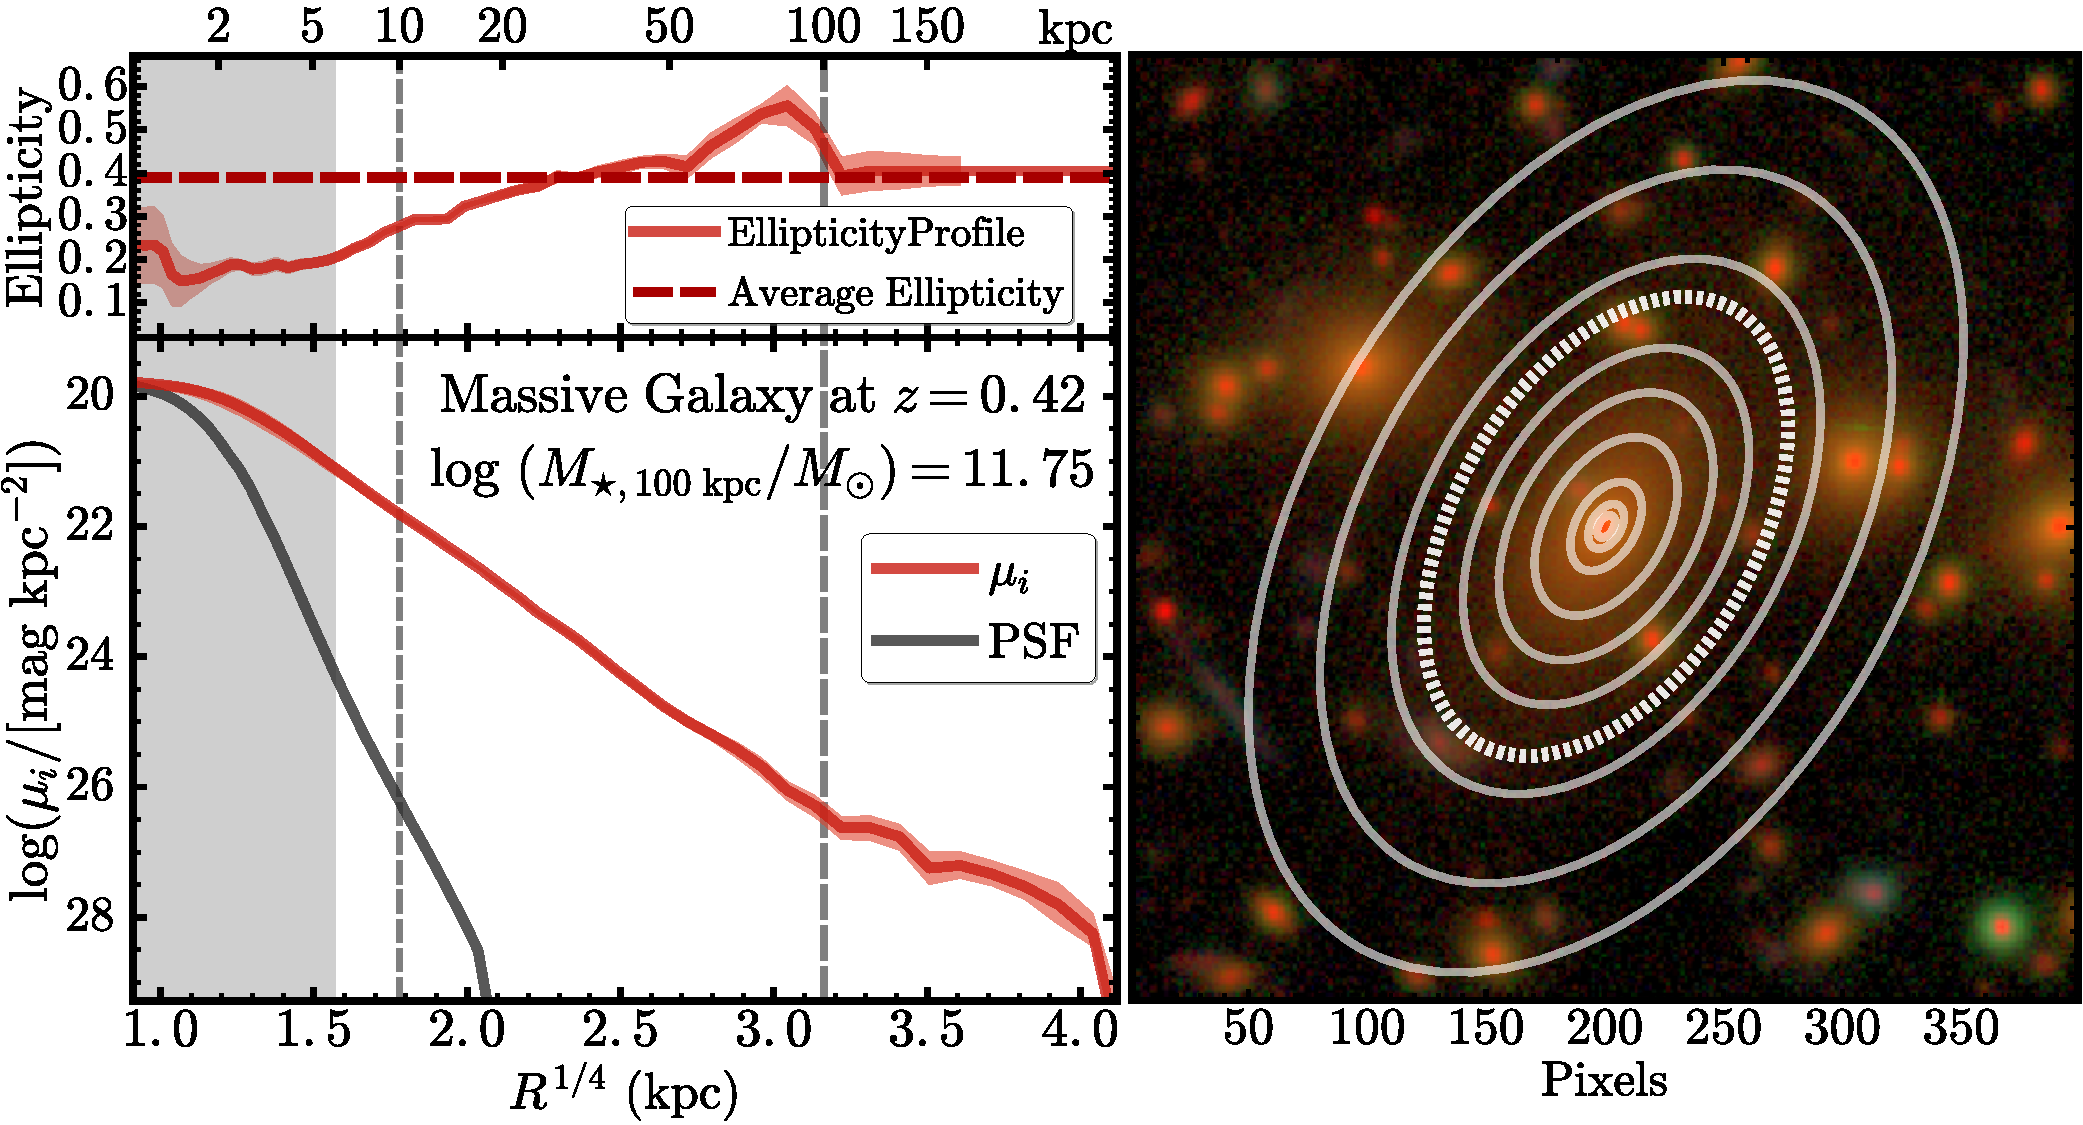
\includegraphics[width=\textwidth]{fig/redbcg_ellipse_example}
        \caption{Left: example of the 1-D surface brightness and ellipticity profile 
            for a massive galaxy at $z=0.23$ in $i$-band using \texttt{Ellipse}. 
            In this work, we always show the radial profile in $R^{1/4}$ scale as it 
            is the most appropriate one to show the structural details of massive 
            ETGs at both inner and outer regions. 
            The dash-line shows the surface brightness profile after correcting the 
            background. 
            We also plot the brightness profile of the PSF model normalized at the 
            central surface brightness of the galaxy to highlight the region affected 
            by seeing. 
            On the top panel, the dash line shows the ellipticity used for the final 
            isophote.~~~ 
            Right: the masked $i$-band image of this galaxy with the isophotes extracted 
            by \texttt{Ellipse} overlaid. 
            The thick, green isophote highlights the one with $\mu_{i}\sim 28.5$~\sb.}
            \song{Will update completely, takes a little bit longer}
            %\alexie{Can we add physical radii at the top left since $R^{1/4}$ is not 
            %    very intuitive. On the right hand side, why show the background as blue, 
            %    instead of showing the actual image of the galaxy with masks overlaid? 
            %    Add units to x axis of right hand side. 
            %    Red text on left hand side, replace with "1D profile of a $10^{xx}$ 
            %    M$_{\odot}$ galaxy at $z=xx$}.}
        \label{fig:ellipse}
    \end{figure*}
%% ------------------------------------------------------------------------------------ %% 

%% ------------------------------------------------------------------------------------ %% 
\section{Data And Sample Selection}
    \label{sec:data}

\subsection{The Hyper Suprime-Cam Survey}
    \label{ssec:hsc}

    The Subaru Strategic Program (SSP, \addref) makes use of the new prime-focus camera,
    the Hyper Suprime-Cam (HSC;~\citealt{Miyazaki2012}), on the 8.2-m Subaru telescope at 
    Mauna Kea. 
    This ambitious multi-layer photometric survey takes advantage of the large field of 
    view (FoV;~1.5 deg in diameter) of HSC and will cover $\sim 1400$ deg$^2$ of sky in 5
    broad bands (\textit{g r i z Y}) to the depth of $r \sim 26$ mag in the \texttt{WIDE}. 
    This work is based on the internal data release \texttt{S15B}, which covers 
    $\sim 100$square of degree of sky in all 5-band to full \texttt{WIDE} depth.  
    The regions covered by this release overlap with a number of spectroscopic surveys 
    (e.g.\ SDSS/BOSS: \citealt{Eisenstein2011}, \citealt{Alam2015}; 
    GAMA: \citealt{Driver2011}, \citealt{Liske2015}).

   The HSC \texttt{WIDE} survey is $3.0$-$4.0$ magnitudes deeper in the $i$-band 
    than SDSS. 
    Combined with the excellent imaging resolution (median $i$-band seeing is 0.6"), 
    and the wide area, this makes the HSC wide layer a tremendous data set to perform a 
    large statistical study of surface brightness profiles of ETGs out to large radii. 
    Fig.\ref{fig:sdss_compare} illustrated the quality of HSC imaging compared to SDSS 
    for a sample of low redshift ETGs. 
    Fig.\ref{fig:sdss_compare} clearly demonstrates that the HSC Wide survey is well 
    suited for mapping the stellar distribution of massive galaxies out to large radii 
    and will be a powerful data set to explore the assembly history of ETGs.

	The HSC $i$-band images typically have the best seeing in all five bands because of 
    strict requirements determined by weak lensing science. 
    We will therefore use the $i$-band images to measure the stellar distributions of 
    massive galaxies. 
    
%% ------------------------------------------------------------------------------------ %% 
\subsection{The HSC galaxy catalog and photometry measurements}
    \label{sec:pipeline}

    The HSC SSP data are processed with \texttt{hscPipe 4.0.1}, a derivative of the Large 
    Synoptic Survey Telescope (LSST) pipeline (e.g.\ \citealt{Juric2015}; 
    \citealt{Axelrod2010}), modified for HSC. 
    \texttt{hscPipe} first performs a number of tasks at the single exposure level 
    (bias subtraction, flat fielding, background modeling, object detection and 
    measurements). 
    Then pipeline perform astrometric and photometric calibration for each single 
    expoures. 
    After that, the \texttt{hscPipe} warp different exposures on to a common
    World Coordinate System (WCS), combine them into coadded images with improved 
    signal-to-noise ratio ($S/N$), and update the images with better astrometric and 
    photometric calibrations at the same time using the common stars among different
    exposures.
    The pixel scale of the combined images is $0.168^{\arcsec}$.  
    The photometric calibration is based on data from the Panoramic Survey Telescope 
    and Rapid Response System (Pan-STARRS) 1 imaging survey 
    (\citealt{Schlafly2012}, \citealt{Tonry2012}, \citealt{Magnier2013}). 
    To achieve consistent deblending and photometry across all bands, \texttt{hscPipe} 
    performs multi-band post-processing at the coadd level. 
    First, the \texttt{hscPipe} performs object detection again on the coadd images
    in each band independently, and identify the above-threshold region (referred as 
    ``footprint'') and the flux peak within it for each source. 
    ``footprints'' and peaks from different bands are then merged together before 
    the \texttt{hscPipe} deblend and measure them in each band. 
    Later, \texttt{hscPipe} selects a ``reference band'' for each object based on the 
    $S/N$ in different bands (for most galaxies in this work, it is the $i$-band). 
    After fixing the centroids, shape, and other non-amplitude parameters of each 
    object in this reference catalog, \texttt{hscPipe} perform forced photometry 
    on the coadd image in each band.
    The PSF and galaxy model fluxes measured in the forced photometry approach are the
    best for color measurements.  
    Please refer to \citet{BoschInPrep} for more details of the \texttt{hscPipe} and 
    the multi-band processing method.    
          
    The HSC \cmodel{} algorithm is similar to the SDSS \cmodel{} one.  
    It fits the flux distribution of an object using a combination of de~Vaucouleur and 
    exponential components after considering the PSF convolution.  
    For more details about the algorithm, please see Bosch\etal~in prep.~.
    We have tested its performance using synthetic objects (Huang\etal~in prep.~), and 
    the results indicate that, generally speaking, the HSC \cmodel{} photometry is 
    accurate down to $i >25.0$ mag.  
    However, for massive ETGs with extended stellar distributions, \cmodel{} currently 
    systematically underestimates their total flux.
    This problem indicates the intrinsic limitation of \cmodel{} as it is incapable of
    modeling profiles that are extremely extended in the outskirt at the depth of 
    HSC survey. 
    At the same time, issues with the deblender also worsen the situation. 
    As the image becomes much deeper, it also significantly increases the fraction 
    objects that are blended with others, and makes reliable deblending process 
    a very challenging problem especially for massive ETGs where satellites and 
    background galaxies often blend with the low surface brightness stellar envelope.
    To make sure the reliable detection of faint objects close to the detection limit, 
    the deblending method implemented by the \texttt{hscPipe} now tends to 
    ``over-deblend'' the surrounding areas of bright galaxies, and further results in 
    under-estimated total flux of massive ETGs (more discussion in 
    Bosch\etal~in prep.~).  
    For these reasons, we will perform customized photometric measurements to derive 
    more accurate total luminosity and stellar mass. 
    We only use the HSC \cmodel{} photometry in the initial selection of parent 
    sample.
    
%% ------------------------------------------------------------------------------------ %% 
\subsection{Initial Massive Galaxy Sample}
    \label{ssec:initial}
    
    Because of the caveats that apply to \texttt{hscPipe} measurements for bright 
    galaxies, we will use custom made software to measure the luminosity profiles of
    massive galaxies. 
    \update{
    As the first step, we select the initial sample of massive galaxies at $z < 0.5$
    from the HSC photometric catalog.}
    We will then use custom made software to re-measure luminosities for all galaxies 
    in this sample. 
    Based on Leauthaud\etal~(2016), most \logms{}$\geq 11.5$ galaxies should have 
    $i_{\mathrm{SDSS, cModel}} \leq 21.0$ mag.
    So we first select all galaxies with $i_{\mathrm{HSC, cModel}} \leq 21.5$ 
    \footnote{We neglect the insignificant differences between the response curves of
    SDSS-$i$ and HSC-$i$ filters}
    in regions that have reached the required depth of \texttt{WIDE} survey in all 
    five bands. 
    %% The SQL search is saved as "sample.sql" 
    %% The master catalog used here is "dr1_wide_galaxy_icmodel_21.5.fits"
    %%   The original catalogs contain 2275477 objects
    
    We select extended objects that have no error in deblending process, well defined 
    centroids, and \texttt{cModel} magnitudes in all five bands. 
    After removing the objects that have pixel affected by saturation, cosmic-ray, and 
    other optical artefact \footnote{each criterion affects less than 8\% of the entire
    sample}, we select 1760845 galaxies that will be referred as \texttt{hscPho}. 
    %% Saved as "dr1_wide_galaxy_hscPho.fits"      
        
    As reliable photometric redshift using HSC photometry is still a working progress, 
    we only use objects with either available spectroscopic redshift or robust 
    red-sequence photo-$z$ from the \redm{} catalog (see Section \ref{ssec:redmapper}).  
    We first match the \texttt{hscPho} sample with the external spec-$z$ catalog 
    compiled by the HSC database\footnote{It is created by matching HSC objects with 
    public data of several spectroscopic surveys (e.g.\ SDSS/BOSS; GAMA). 
    Duplicated matches from different sources are merged through internal matching 
    using $0.5^{\arcsec}$ radius. 
    For each object, the quality information of the spec-$z$ from different catalogs 
    are homogenized into a single flag that indicates whether the redshift is secure, 
    and only secure spec-$z$ are used in this work.}
    %% This is catalog: "dr1_specz_use.fits"
    using $1.0^{\arcsec}$ radius.
    At $0.2 \leq z \leq 0.5$, most redshifts in the HSC spec-$z$ catalog come from 
    SDSS/BOSS and GAMA surveys.  
    The BOSS survey provides the majority of spec-$z$ in this work.  
    Due to the complex selection criteria for different subsamples within the BOSS
    survey (e.g.\ the \texttt{LOWZ} and \texttt{CMASS}), it is not easy to estimate 
    its \mstar{} completeness.  
    Recently, through comparing with the deeper Stripe 82 Massive Galaxy Catalog
    (\texttt{S82-MGC}; \citealt{Bundy2015}), \citet{Leauthaud2016} suggests that the 
    BOSS spec-$z$ is about 80\% complete at \logms{}$\geq 11.6$ at $0.3 < z < 0.5$. 
    The GAMA survey, which partially overlaps with the HSC footprint, provides 
    additional 14\% unique spec-$z$. 
    Based on \citet{Taylor2011} (e.g.\ their Fig.~6), at $z\sim 0.3$, the GAMA 
    sample is 80\% complete down to $10^{10.8}$\msun; but only 80\% complete to 
    $10^{12.0}$\msun at $z\sim 0.5$. 
    Despite the difference in \mstar{} estimates, we can expect 
    our sample should be quite complete above \logms{}$\geq 11.5$-$11.6$.
    We will further address the issue of \mstar{}-completeness more carefully 
    using the common sample with \texttt{S82-MGC} (see Section\ref{ssec:s82}). 
        
    Among the 116813 matched objects, 42696 are at $0.2 \leq z \leq 0.5$.
    %% Saved as "dr1_wide_galaxy_icmodel_21.5.fits"
    The majority of these redshifts come from either SDSS or BOSS data.  
    GAMA survey contributes another $\sim 14$\%. 
    For objects without external spec-$z$, we match them with the central galaxies 
    from \redm{} catalog using $2.0^{\arcsec}$ radius. 
    The matched objects with useful red-sequence photo-$z$ ($z_{\lambda}$) are also 
    included in the final sample of bright galaxies with reliable redshift between 
    $0.2 \leq z \leq 0.5$
    (will be referred as \texttt{hscZ}).
    As we will mention at the end of the paper, to ensure reasonable 
    \mstar{}-completeness at the high-\mstar{} end, and make sure the samples we 
    want to compare have well overlapped redshift distributions, we will focus on 
    the galaxies at $0.3 \leq z \leq 0.5$. 

%% ------------------------------------------------------------------------------------ %%  
\subsection{\redm{}{} cluster catalog}
    \label{ssec:redmapper}
    
    In this paper, our study focuses on galaxies which are located at the center of
    their dark matter halos. To limit our sample to central galaxies, we use 
    \texttt{v5.10} of the \redm{}{} cluster 
    catalog\footnote{See: http://risa.stanford.edu/redmapper/} 
    (e.g.\ \citealt{Rykoff2014}; \citealt{Rozo2015b}). 
    These authors have developed a well-tested red-sequence cluster finder that has been 
    run on SDSS DR8 (\citealt{SDSSDR8}) photometric data. 
    For each cluster, the catalog provides a photometric redshift estimate $z_{\lambda}$, 
    a richness $\lambda$, and identified the most likely central
    galaxy (this is the galaxies with the highest value of the central probability 
    $P_{\mathrm{Cen}}$). 
    A list of member galaxies for each cluster, and associated membership probabilities, 
    is also provided. 
    Details about the performance of the \redm{}~cluster catalog can be found in 
    \citet{Rozo2014}, \citet{Rozo2015a}, and \citet{Rozo2015b}. 
    Several studies have published calibrations between the \redm{}~richness estimate, 
    $\lambda$, and halo mass (e.g.\ \citealt{Saro2015}; \citealt{Farahi2016}; 
    \citealt{Simet2016}). 
    The results of these studies are in good agreement and indicate that clusters 
    identified by \redm{}~($\lambda > 20$) have $\log (M_{200,c}/M_{\odot}) \geq 14.0$. 
    Therefore, the \redm{} catalog helps us group the massive central galaxies into 
    samples with different average \mhalo{}.  
    And, to select reliable candidates of central galaxies, we only include the ones 
    with high probability of being the central galaxy ($P_{\mathrm{CEN}} \geq 0.7$).
       
    Although the \redm{} catalog provides us a good sample of central galaxies in 
    massive halos, the typical uncertainty of $\lambda$ estimate is still at 
    $\sim 5$-10 level.  
    In addition, due to the depth and resolution of SDSS images, the \redm{} catalog 
    becomes slightly incomplete at lower richness ($\lambda < 40$) end at $z > 0.33$.
    To reduce the impacts from uncertain richness and incomplete selection of 
    massive halos, we will focus on a sample of central galaxies in halos with 
    $\lambda > 30$. 
    This will also help up enhance the \mhalo{} contrast in the structural comparison.     
    Based on the calibration in \citet{Simet2016}, the $\lambda \geq 20$ sample should
    have halo mass ($M_{200m}$) more massive than $10^{14.0} M_{\odot}$.  
    For the $\lambda \geq 30$ sample, they should live in halo more massive than
    $10^{14.2} M_{\odot}$ using the same calibration. 
    And, we can confirm that the results presented later do not depend on the choice 
    of $\lambda$ boundary here. 
    For the massive central galaxies that are not in these cluster-level halos, 
    we unfortunately can not estimate their \mhalo{} individually, but it is safe 
    to assume they should have $\log (M_{200m}/M_{\odot}) < 14.0$.     
    %\textcolor{red}{but sometimes we make cuts at $\lambda<20$ and $\lambda>30$. 
    %Is it confusing to have several different thresholds? Need to give a Motivation 
    %for using different numbers here.}
    
%% ------------------------------------------------------------------------------------ %% 

%% ------------------------------------------------------------------------------------ %% 
  \begin{figure*}[bt!]
      \centering 
      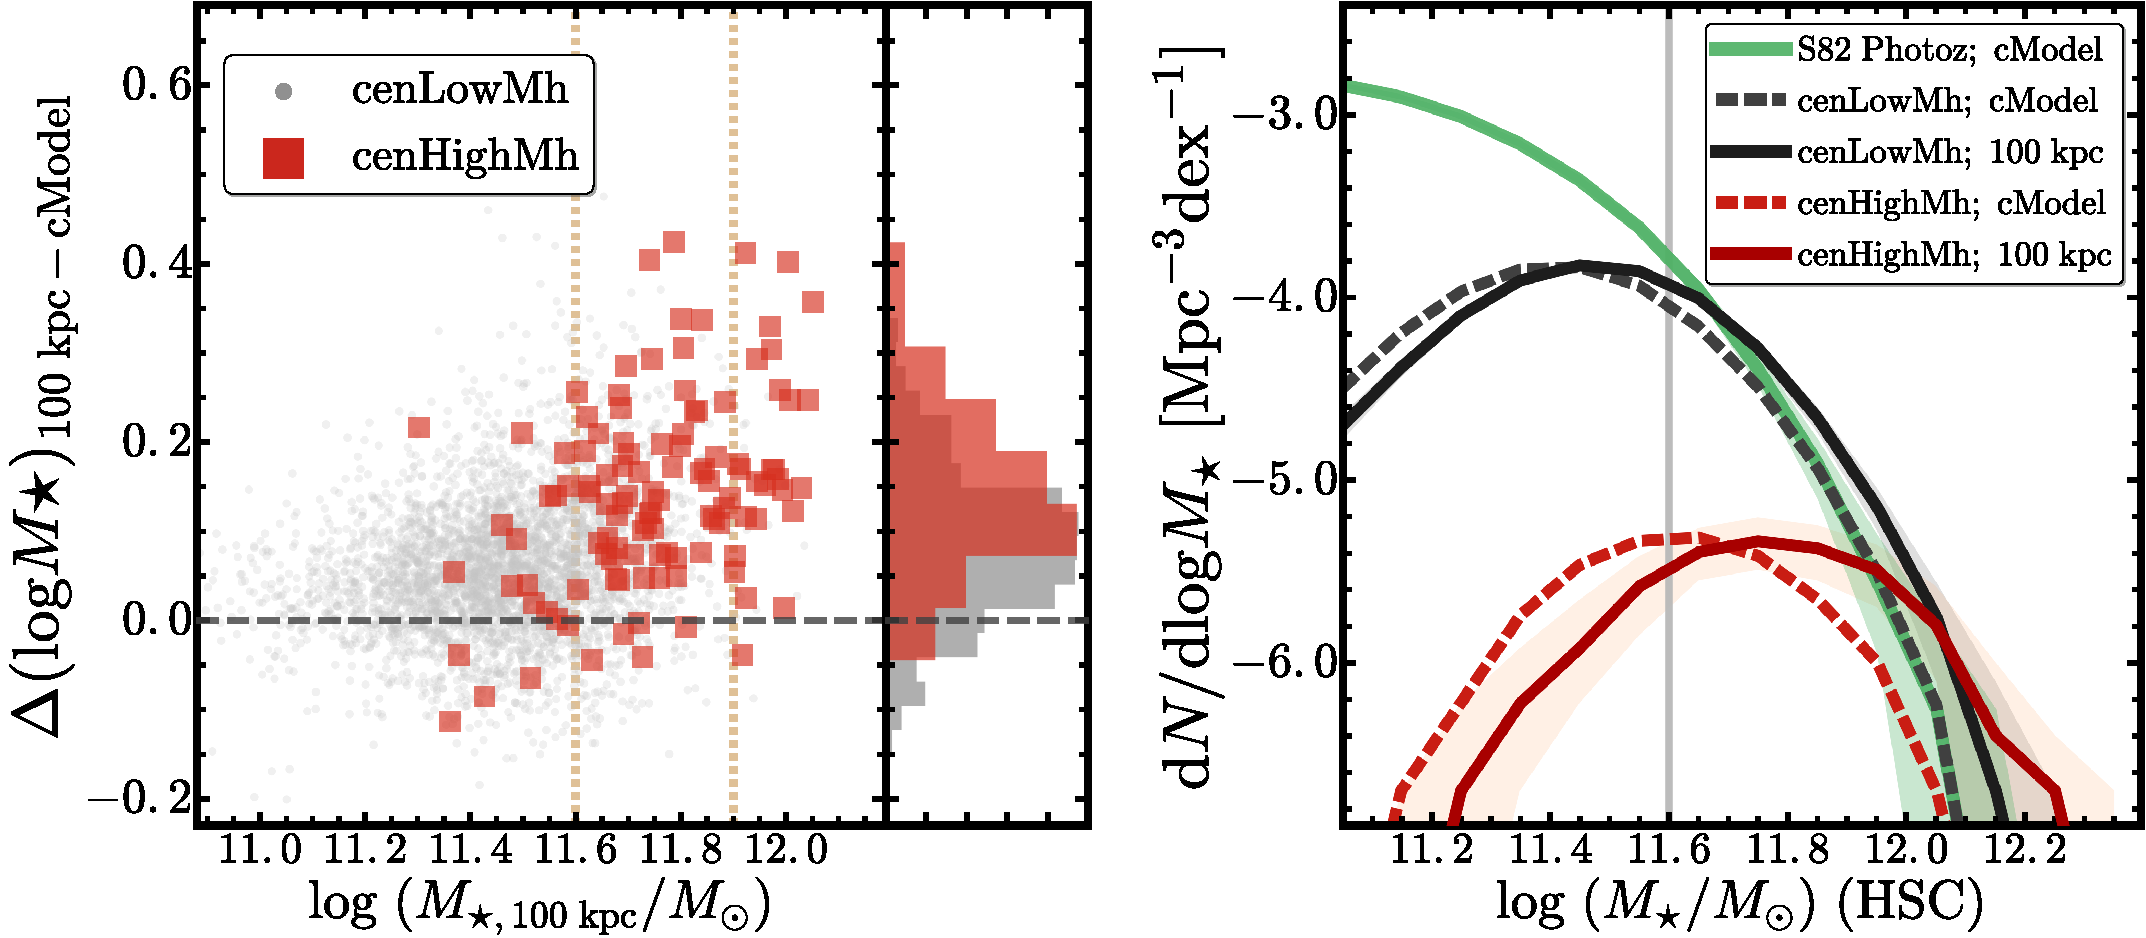
\includegraphics[width=\textwidth]{fig/redbcg_smf_new}
      \caption{\textbf{Left:} Difference between \mcmodel{} and \mtot{} for central
      	galaxies in halos smaller than $10^{14}$ M$_{\odot}$ (grey dots) and in
        halos larger than $10^{14}$ M$_{\odot}$ (red squares). 
        On average, \mcmodel{} underestimates the total stellar mass of massive 
        galaxies by 0.1 dex and the difference can exceed 0.2 dex. 
        Vertical histograms indicate the mass difference for galaxies with
        $11.6<$\logmtot{}$<11.9$. 
        \textbf{Right:}: Impact of using \mcmodel{} on the galaxy stellar mass
        function. 
        Dashed lines correspond to the SMF computed using \mcmodel{} as an estimate
        of the total luminosty whereas solid lines correspond to the SMF computed
        using the total luminosity from our 1-D profile modeling. 
        The impact on the SMF can exceed 0.2 dex for massive centrals living in
        halos larger than $10^{14}$ M$_{\odot}$ (red lines).}
      \label{fig:smf1}
  \end{figure*}
  
%           We compre the \mstar{} volume-density distributions of 
%      	  \rbcg{} (red) and \nbcg{} (black) galaxies using stellar mass based on 
%          \mcmodel{} (dash) and \mtot{} (solid) to highlight the increase of \mstar{}
%          due to different methods.  
%          Here we also show the volume-density distributions of the \texttt{S82-MGC} 
%          galaxies (green) to evaluate the \mstar{}-completeness. 
%          The vertical line highlight \logms{}$=11.6$ before correcting the \mstar{} using
%          total luminosity from 1-D profile.~~
          
%% ------------------------------------------------------------------------------------ %%
 
%% ------------------------------------------------------------------------------------ %% 
\subsection{Massive Central Galaxies from Low and High Mass Halos}
    \label{ssec:mass_central}
    
    Based on recent constraints of $M_{\star}$-$M_{\mathrm{Halo}}$ relation 
    (e.g.\ \citealt{Leauthaud2012}, \citealt{Behroozi2013}, \citealt{Kravtsov2014}), 
    the \mhalo{} of \logms{}$ > 11.0$ galaxies has a large scatter at fixed \mstar{}.            
    Although we can not yet measure \mhalo{} individually, we can still broadly 
    separate them into galaxies in small groups (\logmh{}$<14.0$) and 
    large groups/clusters (\logmh{}$>14.0$), and investigate the 
    ``environmental''-dependence of their structures. 
    
    % We match this sample with the central galaxies of \redm{}~catalogs using a 
    % $1.0^{\arcsec}$ radius, and it results in 704 galaxies.  
    %% Saved as "dr1_redbcg_hsc_sdss_gama_1arcsec.fits"
    Firstly, we match the \texttt{hscZ} sample with the massive central galaxies of 
    \redm{} clusters with $\lambda \geq 20$ and $P_{\mathrm{0.7}} \geq 0.7$ using 
    $1.0^{\arcsec}$ radius. 
    This step finds 375 matched galaxies at $0.2 \leq z \leq 0.5$ 
    (among them 282 are at $0.3 \leq z \leq 0.5$).  
    We will refer these \textbf{central galaxies in more massive halos} as \rbcg{} 
    sample from now on.
    A small fraction of \redm{} centrals within the HSC footprints are missing  
    due to severe contamination from optical artifacts or bright stars.
    Spec-$z$ is not available for 67 (17.9\%) galaxies in the sample, but their 
    $z_{\lambda}$ should be very accurate (median $|z_{\lambda} - z_{\mathrm{Spec}}|$ is 
    about 0.01 for the ones with spec-$z$).
    The median richness ($\lambda$) of these clusters is $\sim 32$, corresponding to 
    halo mass of $M_{200m}\sim 1.7\times 10^{14} h^{-1} M_{\odot}$. 
    Among these central galaxies, 222 are in clusters with $\lambda \geq 30$. 
    When focusing on this subsample, the median richness is $\sim 41$, corresponding 
    to halos with $M_{200m} \sim 2.2\times 10^{14} h^{-1} M_{\odot}$. 
    Meanwhile, only 15\% of \rbcg{} sample lives in clusters with $\lambda \geq 50$
    ($M_{200m} \sim 3.0\times 10^{14} h^{-1} M_{\odot}$).   
    Therefore, the current \rbcg{} sample is not dominated by very massive clusters 
    with \mhalo{}$>10^{15} M_{\odot}$.  
    %% Saved as "dr1_redbcg_use_sed5b.fits"
    
    Assuming that the \redm{} catalog correctly identifies all halos with 
    $M_{200m}\sim 1.0\times 10^{14} h^{-1} M_{\odot}$ in the current footprint,
    the unmatched massive galaxies from the above step should be dominated by central 
    galaxies of less massive halos and massive satellites galaxies.  
    \update{
    To select a purer sample of massive centrals in $M_{200m}<10^{14} h^{-1} M_{\odot}$
    halos, we identify and remove all galaxies within a cylinder region around the 
    the central galaxies in \redm{} catalog.
    We choose to use the $R_{200m}$ as the radius of the cylinder. 
    For each cluster, we convert the richness estimates into $M_{200m}$ using the 
    calibration in \citep{Simet2016}, then estimate the $R_{200m}$ using $M_{200m}$
    and the mass-concentration relation in \citep{Diemer2015}. 
    For the thickness of the cylinder, we use twice the uncertainty of the photometric 
    redshift error of each cluster.  
    At $0.3 < z < 0.5$, such uncertainty is between 0.015 to 0.025, which are more than 
    enough to exclude cluster member.}
    \song{The actual number waits to be updated}
    
    %\alexie{This is a rather strange procedure, I think we need to change it (referee and readers will complain!). What we really want to do is to remove any galaxies that have $r<R200$ in projection (from the galaxy with the highest value of Pcen) and remove galaxies within some deltaz of the cluster redshift. The cluster redshift is more well determined than the redshift estiamte of any cluster member. In short, what we are doing here is cutting out a cylindar arond the most likley BCG. The deltaz value can be motivated by the cluster redshift uncertainty from the redmapper papers. The only remaining question is then what radius to use around clusters. To get that number here is what we need to do. 1) Start with Eq 12 and Table 3 in Simet et al. For each cluster, assign a value of M200m (halo mass defined as 200 time background) to each cluster. 3) we then need to estimate the cluster radius R200m (or R200b, same thing). To do this, we need to use a mass-concentration relation. I'm pretty sure there is an easy command to do this in Python using the python package "colossus" by bendikt diemer. Download it and see if youc an get it to work. If it doens't look obvious after 30 min, I can do it on my end using my own code. But good for you to know how to do this. We can simply use the mass-concentration realtion from Benedikts work. 4) Now for every cluster you have R200m. And you define the low halo mass central sample as ones that are not within any cylindar around any cluster. Sorry, I know this might mean re-doing everything.....let's discuss by Skype if this is a major issue.}
    
    However, we should note that the \nbcg{} sample at this stage spans a large range
    in \mstar{}, extending towards \logms{}$<10^{11}$.  
    Therefore, we should expect contamination from satellites in \logmh{}$< 14.0$ halos
    at certain degree.  
    Later, after we update the total \mstar{} of them, we will mainly focus on the 
    \nbcg{} galaxies at high mass end, especially the ones at \logms{}$ > 11.5$. 
    Based on observational constraints (e.g. \citealt{vanUitert2016}), we can neglect 
    satellite contamination at such high \mstar{} range. 
    %% Saved as "dr1_nonbcg_use_sed5b.fits"

\subsection{Summary of Sample Construction}
    \label{ssec:sample}

    In summary, from the $\sim 100$ deg$^2$ deep HSC images, we select a large sample
    of massive central galaxies with reliable redshift information, and broadly separate 
    them into two groups with different \mhalo{}.  
    To help you go through the results, here are a few key points to keep in mind:
    
    \begin{itemize}
        \item \texttt{hscPho} sample: this parent sample consists of bright galaxies 
            with $i_{\mathrm{cModel}} \leq 21.0$, good quality images and reliable 
            \texttt{cModel} photometry in all five HSC bands in the \texttt{S15B} 
            data release. 
        \item \texttt{hscZ} sample: through matching the \texttt{hscPho} sample with 
            spectroscopic redshifts from surveys like SDSS/BOSS and GAMA, or accurate 
            red-sequence photometric redshift in the \redm{} catalog, we come up with 
            a large sample of bright galaxies with reliable redshift information. 
        \item \rbcg{} sample: we select a sample of 375 galaxies at $0.2 \leq z \leq 0.5$
            that are identified as central galaxies in $\lambda > 30$ \redm{} clusters. 
            The most reliable ones ($P_{\mathrm{Cen}} >0.7$) among 
            them will represent the central galaxies in very massive halos
            (\logmh{}$\geq 14.0$). 
        \item \nbcg{} sample: after excluding all the galaxies that are close to any 
            \redm{} clusters in both radial and redshift directions from the 
            \texttt{hscZ} sample, we have 29973 bright galaxies at $0.2 \leq z \leq 0.5$.
            With the help of \mstar{} estimates via SED fitting (see Section 
            \ref{ssec:isedfit}), we consider the massive ones among them as the 
            candidates of central galaxies in halos with \logmh{}$<14.0$.  
        \item To compare the \rbcg{} and \nbcg{} samples carefully, we will focus on 
            the redshift range at $0.3 \leq z \leq 0.5$ where their redshift 
            distributions greatly overlap and both samples have acceptable
            \mstar-completeness (see Section \ref{ssec:s82}).  
            \update{Although we use the $\lambda > 30$ sample for structural comparison, 
            in the Appendix.\ref{app:robust}, we show that the results will not change 
            if we include central galaxies of $20 < \lambda \leq 30$ clusters in the 
            \rbcg{} sample.}
    \end{itemize}

%% ------------------------------------------------------------------------------------ %% 


%% ------------------------------------------------------------------------------------ %% 
\section{Measurements of 1-D Surface Brightness Profile}
    \label{sec:ellipse}
    
    To estimate the total luminosity of massive galaxies, and measure their 
    one-dimensional stellar mass density (\mden{}) profiles, we perform elliptical 
    isophotes fitting using the IRAF task \texttt{Ellipse} (Jedrzejewski 1987).  
    Compared to the popular two-dimensional model fitting method, the isophote fitting
    approach is much less sensitive to the choice of model, number of components, 
    and the initial guesses of free parameters. 
    It is also less affected by the uncertainty of sky background subtraction.  
    This is particularly important for the massive ellipticals in our sample.  
    The much deeper HSC image reveals significantly more extended structures, 
    while also make it inappropriate to fit these galaxies with simple model like 
    the de~Vaucouleurs model or single \ser component model. 
    Such models fail to fit the central region and the stellar halo of massive 
    galaxies simultaneously, and also can not account for the radial variation of 
    ellipticity and position angle. 
    In principle, such massive galaxies can still be described using more complex 
    models (e.g \citealt{Huang2013a}; \citealt{Huang2013b}).  
    However, they are still very sensitive to background subtraction. 
    And it becomes even more difficult to choose initial parameters, and investigate
    the degeneracies among parameters. 
    Although it is certainly worth exploring in the future, we decide that the 1-D 
    method suits the goal of this work better.
        
    We first prepare large $i$-band cut-out images around these massive galaxies 
    that cover at least 750 kpc in radius, along with the bad pixel masks, and the 
    PSF model reconstructed using the central coordinates. 
    While they include all the visible light of the galaxy, they also leave enough 
    space to evaluate the background subtraction. 
    We choose to use $i$-band images not only considering their excellent seeing
    condition, but also because they trace the stellar distributions of massive 
    galaxies at $0.3 \leq z \leq 0.5$ reasonably well (fall between rest-frame $g$ 
    and $r$ band), and they suffer less from background uncertainty, which is crucial 
    for studying the outskirt of massive ETGs.  
    Although $z$ and Y-band should be better \mden{} tracer, the sky background 
    is much higher and the seeing is considerably worse on average. 
    
    Secondly, using the \texttt{SEP} Python library, we perform \texttt{SExtractor}-like
    background estimation and object detections using different configurations to 
    overcome the ``over-deblending'' challenge met by the \texttt{hscPipe}. 
    Combining detections using different backgrounds and $S/N$ thresholds, 
    we correctly obtain the footprints of all objects, even of the ones that are 
    very close to the center of bright galaxies.
    For the rest objects, we convert their footprints into a mask image for the
    \texttt{Ellipse} procedure after increasing their sizes adaptively based on the 
    brightness and distance to the massive galaxy. 
    We achieve this via convolving the individual footprint with a Gaussian kernel
    so that we can conservatively exclude pixels affected by this object while still 
    making the mask follow the shape of the object. 
    Meanwhile, we create a more aggressive mask of \emph{all} objects in the same 
    approach, median-rebin the remaining pixels using a $6x6$ pixels box, and take 
    the peak value (or mode) of the distribution of these rebinned ``sky'' pixels 
    as the average background value around these bright galaxies.
    As expected, we often found slightly negative value that indicate over-subtraction 
    of background at certain degree. 
    In \texttt{hscPipe}, the background on each CCD is modeled with a 
    Chebyshev-polynomial fit to the smoothed image after excluding pixels with $S/N >5$.
    This algorithm suffer less than the SDSS version (e.g.\ see \citealt{Blanton2011}),
    but still over-subtract background around very bright object. 
    For our massive galaxies, such over-subtracted background creates artifactual
    truncation or steeper surface brightness profile.
    We therefore provide an ad hoc fix using a \texttt{SExtractor}-style background 
    model ($200x200$ pixels background box size, and 6 pixels median filtering size of 
    sky boxes) via running \texttt{SEP} on the image with all objects masked out.
    This model can account for the slightly over-subtracted background at very large 
    scale, shift the distribution of rebinned ``sky'' pixels to 0, and do not affect the 
    intrinsic flux distribution of our target. 
    
    Finally, we run \texttt{Ellipse} on the background-corrected image following similar 
    strategy of \citep{Li2012}.
    In short, we start with free centroid and shape of each isophote, then gradually 
    constrain their behaviors, and eventually extract 1-D surface brightness profile 
    along the major axis using isophotes with fixed centroid and shape.
    The 4th Fourier modes are included to fit the isophote better. 
    In this way, we can extract the radial changes of the centroid, ellipticity, 
    position angle, and average isophotal distortions (more ``disky'' or ``boxy'', 
    e.g.\ \citealt{Kormendy2009}) along with the surface brightness profile.  
    Fig.\ref{fig:ellipse} shows an example of the 1-D surface brightness and 
    ellipticity profile for a massive galaxy at $z\sim0.2$ along with its masked 
    image and a subset of isophotes.  
    Appendix.\ref{app:A} includes more details about the \texttt{Ellipse} procedure.
    
    %At low surface brightness regime, the final profile can be sensitive to several 
    %configuration parameters of \texttt{Ellipse}.  
    %After some tests, we choose to use 0.1 dex in logarithm as the step in semi-major 
    %axis length between successive ellipses, and we use the median pixel value over the
    %elliptical annulus after rejecting outlier pixels twice with $3\sigma$-clipping.
    %These parameters are selected to make the final profile less affected by any nearby
    %objects, and please see Appendix.~B for more details about the extraction of 
    %1-D profile. 
        
    For physical (e.g.\ late-stage major merger) and unphysical (e.g.\ nearby 
    foreground galaxy or bright star) reasons, we can not extract reliable 1-D 
    profiles for small fraction of massive galaxies due to heavily masked out 
    central region. 
    This issue reflects an intrinsic limitation of the 1-D method. 
    It affects $48/375$ \rbcg{} galaxies, and a smaller fraction of \nbcg{} ones. 
    It is worth noting that this excludes most massive galaxies in major merger 
    process from the analysis. 
    We will come back to them in the future using 2-D modeling method.
    
    We correct these surface brightness profiles for Galactic extinction and 
    cosmological dimming, then integrate them to various radius to get the 
    luminosity within different physical apertures.  
    Although the $i$-band 1-D profile can in principle reach to $\sim 30$ \sb, 
    we notice the profiles at very low surface brightness part are often less 
    reliable by showing truncation or large fluctuation that are due to either 
    background uncertainty or contamination from bright neighbours.
    We therefore only consider the $<28.5$ \sb part of the profile here. 
    This conservative choice already allows us to study the region out to 
    $\sim 120$ kpc for massive galaxies in this sample.  
     
    %We also apply the isophotes from $i$-band images to other bands in 
    %``force-photometry'' mode \texttt{Ellipse} run to get rough estimates of 
    %color profiles.  
    %Without taking the difference in seeing and background into account, 
    %these color profiles can not be used for physical discussion. 
    %But with the help of $K$-correction from the next section, we show that there 
    %is no systematic difference in color gradient between \rbcg{} and 
    %\nbcg{} sample. 
    
%% ------------------------------------------------------------------------------------ %% 

\section{Stellar Masses and Stellar Mass Density Profiles}
    \label{sec:mstar}
    
\subsection{Stellar Masses from SED Fitting}
    \label{ssec:isedfit}
   
    To convert the luminosity into stellar mass estimates, we assume that these massive 
    galaxies can be well described by an average \m2l{}. 
    This is a reasonable assumption considering that they are ETGs that are dominated by 
    old stellar population and are known to have shallow color gradients. 
    We will further justify this point using the average color profiles in Section
    \ref{sec:discussion}.

    We use the broadband Spectral Energy Distributions (SEDs) fitting 
    (see \citealt{Walcher2011} for a recent review) code 
    \texttt{iSEDFit}\footnote{http://www.sos.siena.edu/~jmoustakas/isedfit/} 
    (\citealt{Moustakas13}) to estimate the average \m2l{} and $k$-corrections using
    5-band HSC \cmodel{} fluxes under forced-photometry mode. 
    Although \cmodel{} tends to underestimate the total flux for bright, extended 
    objects, the forced-photometry results still provides accurate \emph{average} color 
    of the galaxy as it constrains the behaviour of the model using the optimized 
    reference one and taks the PSF convolution into account
    (e.g.\ Huang\etal~in prep.~). 

    \texttt{iSEDFit} takes a simplified Bayesian approach. 
    In short, it first generates a large grid of SEDs from synthetic stellar population 
    models by drawing randomly from the prior distributions of relevant parameters 
    (e.g.\ age, metallicity, dust extinction, and star formation history).
    Based on these models, it uses the observed photometry and redshift to compute the 
    statistical likelihood, and generate the posterior probability distribution (PDF) 
    functions of each parameter.  
    To get the best estimate of certain parameter, \texttt{iSEDFit} ``integrates'' the 
    full PDF over all the other ``nuisance'' parameters.
    Then, the median value of the resulting marginalized PDF is used as the best value, 
    while the 1-$\sigma$ uncertainty is derived from the cumulative PDF. 
    Please refer to \citet{Moustakas13} for technical details and performance of 
    \texttt{iSEDFit}. 
    
%% ------------------------------------------------------------------------------------ %% 
    In this work, we derive average \m2l{} using the Flexible Stellar Population 
    Synthesis\footnote{http://scholar.harvard.edu/cconroy/sps-models}
    (FSPS; \texttt{v2.4}; \citealt{FSPS}, \citealt{Conroy2010}) model based on the MILES
    \footnote{http://www.iac.es/proyecto/miles/pages/stellar-libraries/miles-library.php}
    (\citealt{MILES1}, \citealt{MILES2}) stellar library and \citet{Chabrier2003} 
    IMF between 0.1 to 100 \msun. 
    We use a delayed-$\tau$ model with stochastic star burst as the form of star 
    formation history (SFH), and choose a set of reasonable parameters after some tests.  
    Such form of SFH is appropriate for massive galaxies at low redshift 
    (e.g.\ \citealt{Kauffmann2003}). 
    For stellar metallicity, we assume flat distribution between 0.004 to 0.03 (which is 
    the highest metallicity allowed by FSPS models).  
    And, we adopt the \citet{Calzetti2000} extinction law with a order two Gamma 
    distribution of $A_{V}$ between 0 to 2 magnitude.
    Since most galaxies in both samples are red, quiescent galaxies, the results are 
    not very sensitive to parameters related to SFH and internal dust extinction. 
    To achieve reasonable sampling across these parameters, we generate 250000 models. 
    
    We construct five band SED using the forced-photometry \cmodel{} magnitude corrected 
    for the Galactic extinction. 
    As for the photometric error, the current \cmodel{} photometry underestimates 
    the flux errors of bright galaxies as it only includes statistical error, not the 
    systematic uncertainties in the model-fitting process.  
    From tests of synthetic objects, we find that the average accuracy of \cmodel{} 
    photometry for bright galaxy is roughtly at 1\% level. 
    Therefore, we supply \texttt{iSEDFit} with simplified flux errors assuming $S/N = 100$ 
    for $riz$ bands, and $S/N = 80$ for $gY$ bands (on average, images in $gY$ bands are 
    shallower in depth and/or have higher background noise).  
    The typical uncertainty of \logms{} for both samples is around 0.08-0.10 dex at the 
    high-\mstar{} end. 
    Please see Appendix.\ref{app:B} for more detailed discussions of the SED fitting
    results.  
    %In Fig.~3, we show an example of SED fitting result. 
    %\song{Not sure if we need to show one example, but put one here for now.}
    
%% ------------------------------------------------------------------------------------ %% 
    
\subsection{Comparison with \texttt{S82-MGC}}
    \label{ssec:s82}

    Given the heterogeneous nature of the redshift resources for these samples, we 
    further investigate their \mstar{} completeness via comparing with galaxies that are 
    in common with the \texttt{S82-MGC} sample. 
    The \texttt{S82-MGC} sample matches the deeper SDSS photometric data in the Stripe 82 
    region (\citealt{Annis2014}) with the near infrared data from the United Kingdom 
    Infrared Telescope Infrared Deep Sky Survey (UKIDSS; \citealt{Lawrence2007}). 
    The deeper photometry and better photo-$z$ make the \texttt{S82-MGC} sample complete 
    to \logms{}$\geq 11.2$ at $z<0.7$.  
    
    The match between the \texttt{hscPho} sample and the \texttt{S82-MGC} one results in 
    20453 galaxies at $0.3 \leq z \leq 0.5$ (referred as \texttt{s82Pho} sample).  
    We estimate their \mstar{} using \texttt{cModel} SED in exactly the same way. 
    The \mstar{} using HSC photometry shows tight correlation with ones based on the
    \texttt{S82-MGC} SED (five optical bands from SDSS and NIR data from UKIDSS; and 
    \texttt{S82-MGC} also used \texttt{iSEDFit} under slightly different assumptions).  
    Then we estimate the volume densities distributions of galaxies in \rbcg{}, \nbcg{}, 
    and \texttt{s82Pho} samples (left panel of Fig.\ref{fig:smf1}) using rough estimates 
    of the survey areas they occupied (since we only care about the relative shapes of 
    the density distributions). 
    And, we estimate the uncertanties of these distributions using a 10000 times 
    bootstrap resampling. 
    The distribution of \nbcg{} sample starts to deviates from the \texttt{s82Pho} one 
    below \logms{}$< 11.6$, indicating that the sample starts to become incomplete within
    $0.3 \leq z \leq 0.5$. 
    As for the \rbcg{} sample, their mass completeness should be better thanks to the 
    reliable \redm{} $z_{\lambda}$. 
    Its behaviour is quite consistent with the mass function of galaxies in massive 
    halos with a narrow \mhalo{} distribution (\addref).   
    Later, we will see that the \cmodel{} photometry on average underestimate the 
    \mstar{} of galaxies with \logms{}$>11.5$ by $-0.1$ dex.
    Therefore, we conclude that the \nbcg{} becomes not perfectly complete below 
    \logms{}$< 11.7$.  
    This is most likely due to the incompleteness of the BOSS spec-$z$ sample. 
    Although it is unlikely that the incompleteness will bias the results of our 
    comparisons, we will bear this in mind, and match the two samples carefully in 
    \logms{} and redshift space before comparing them.

%% ------------------------------------------------------------------------------------ %% 

%% ------------------------------------------------------------------------------------ %% 
  \begin{figure*}[bt!]
      \centering 
      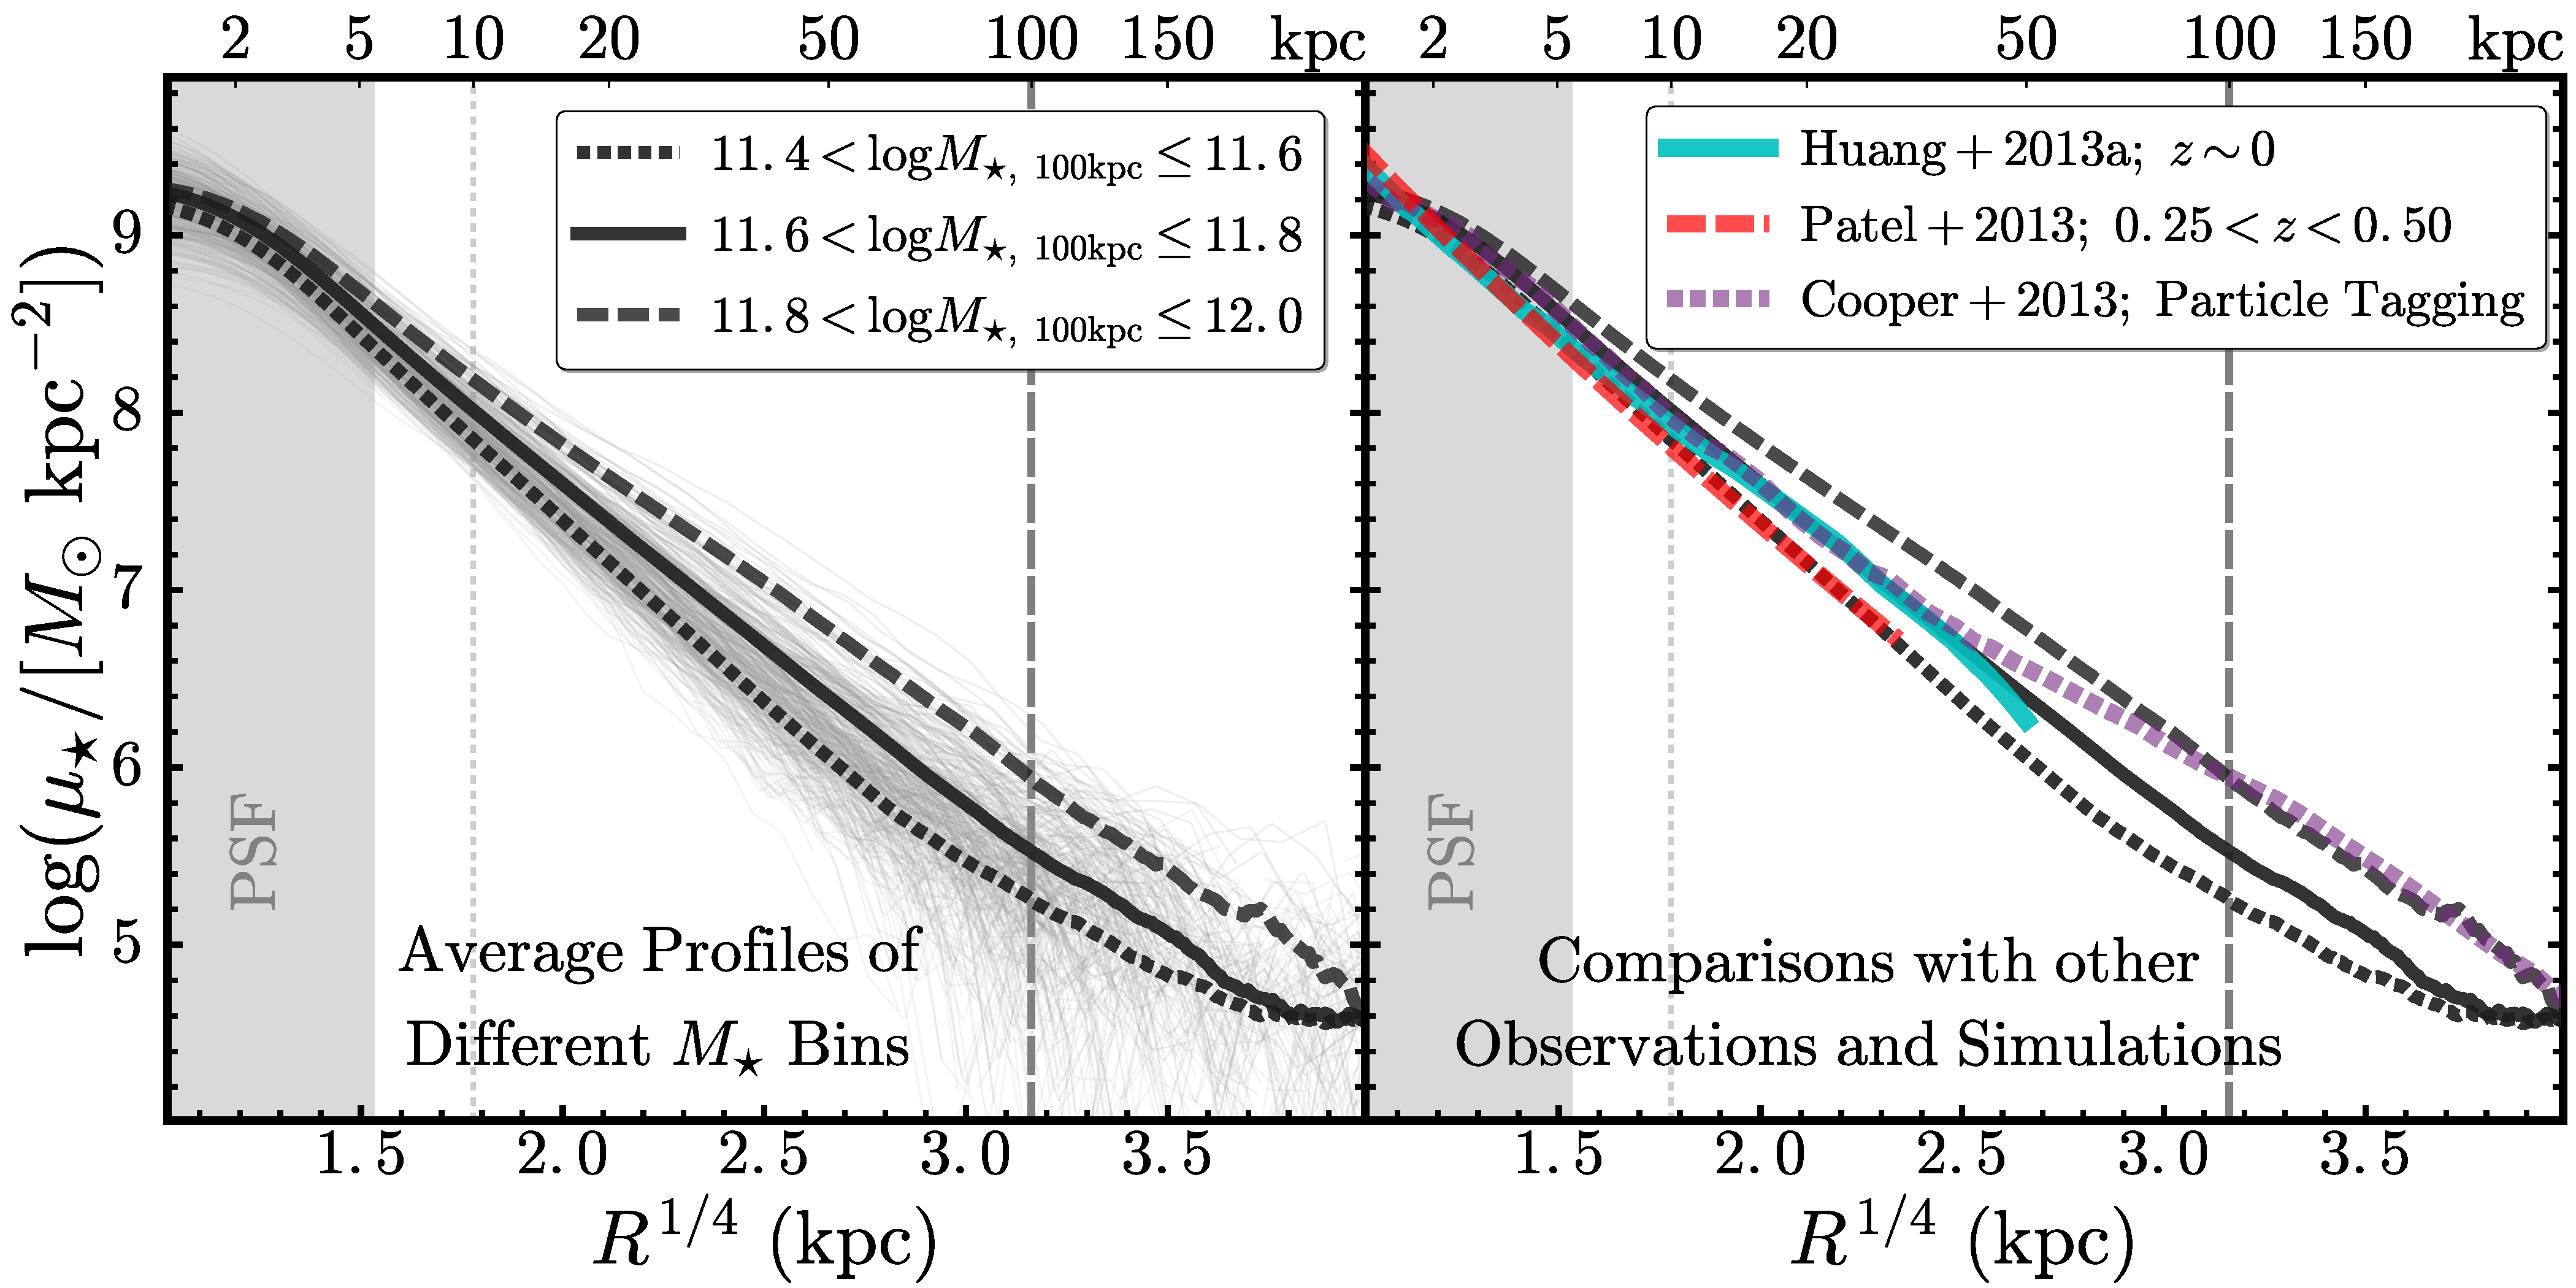
\includegraphics[width=\textwidth]{fig/average_mass_profiles_fsps1_A}
      \caption{
      	\textbf{Left}: Median \mden{} profiles of galaxies in different \mtot{} bins:
      	[11.4, 11.6] (short-dashed line), [11.6, 11.8] (solid line), and 
      	[11.8, 12.0] (long-dashed line). 
      	Here we combine the \rbcg{} and \nbcg{} samples, and we also show a random subset 
      	of individual profiles in the background.
      	The shaded region highlights the region that could be affected by PSF.
        Two vertical lines label the radius of 10 kpc (thin, dotted line) and
        100 kpc (thick, dash line). ~~~ 
        \textbf{Right}: comparison between the average \mden{} profiles with the ones 
        from previous observations and simulations, including: 
        1) average profile of massive elliptical galaxies at $z\sim 0$ from 
        \citet[][Cyan, solid]{Huang2013a}; 
        2) average profile of massive galaxies at $0.25 \leq z < 0.50$ observed by 
        \textit{HST} from \citet[][Red, long-dashed]{Patel2013} ;
        3) average radial stellar distribuitions in massive halos using simulation and 
        particle tagging method (\citealt{Cooper13}; Purple, short-dashed).}
      \label{fig:avg_prof}
  \end{figure*}
%% ------------------------------------------------------------------------------------ %% 

%% ------------------------------------------------------------------------------------ %% 
  \begin{figure*}[t!]
      \centering 
      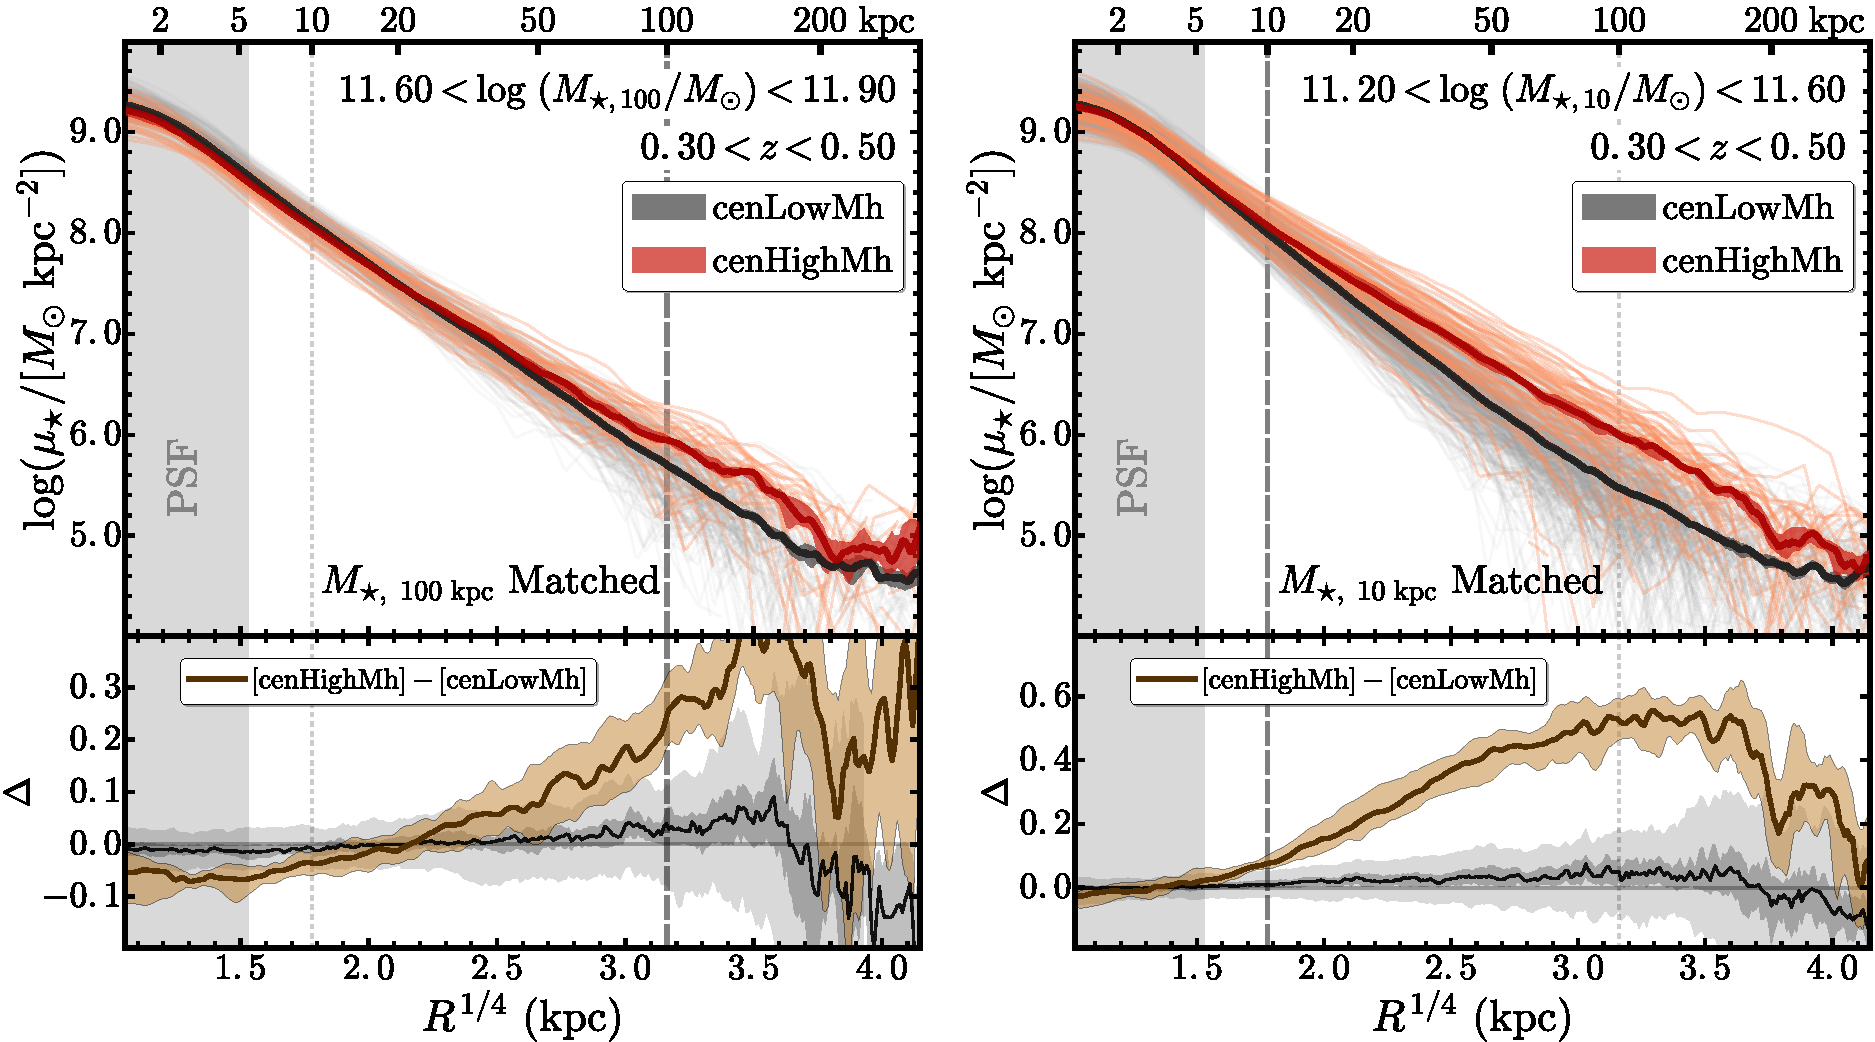
\includegraphics[width=\textwidth]{fig/redbcg_prof_1}
      \caption{
          \update{
          Comparison of the \mden{} profiles for \mtot{}-matched ($11.6<$\logmtot{}$<11.9$) 
          and \minn{}-matched ($11.2<$\logminn{}$<11.6$) samples 
          of \rbcg{} (orange to red) and \nbcg{} (grey to black) galaxies.~~
          \textbf{Left} shows the results for the \mtot{}-matched samples.
          For details of the matching process, please see Appendix.\ref{app:match}.  
          On its upper panel, we show the \mden{} profile of each galaxy using very light 
          color in the background.  
          We highlight the median profile and its corresponding uncertainties using thick 
          solid line with darker color and shaded region. 
          Other formats are the same with Fig.\ref{fig:avg_prof}.
          Meanwhile, we highlight the difference between the median profiles and its 
          uncertainty on the bottom panel (brown solid line and shaded region).
          To test the significance of the differential profile, we perform statistical tests 
          by comparing the median profiles of two random groups that are drawn from the 
          mixed sample, and have the same sizes with the matched \rbcg{} and \nbcg{} ones.
          Repeating this process many times, the median of these random differential 
          profiles (black solid line), the 1-$\sigma$ (dark-grey shaded region) and 3-$\sigma$
          (light-grey shaded region) uncertainties are shown on the bottom panel as well. 
          A darker vertical dash-line highlights the 100 kpc radius.~~
          \textbf{Right} shows the results for the \minn{}-matched samples. 
          The format is exactly the same with the left one, except that the darker vertical 
          dash-line now highlights the 10 kpc radius.}
      }
      \label{fig:prof_1} 
  \end{figure*}
%% ------------------------------------------------------------------------------------ %% 

\subsection{Stellar Mass Corrected for Total Luminosity}
    \label{ssec:mtotal}
    
    Using the best-fit stellar mass from \texttt{iSEDFit} (referred as \mcmodel{}), 
    we estimate the average \m2l{} in $i$-band, then use that \m2l{} to convert the 
    1-D luminosity density profiles into stellar mass density profiles; and 
    also convert the luminosity within 10 and 100 kpc apertures into 
    corresponding stellar mass estimates (referred as \minn{} and \mtot{}). 
    From now, we use \mtot{} as the new proxy of ``total'' stellar mass of these 
    galaxies.  
    And we also derive the $k$-corrected luminosity and colors from the results.
    In Appendix.\ref{app:B}, we also show the outputs like the average stellar age, 
    metallicity, and internal dust extinction all behave reasonably for both 
    samples, but will not use them for further scientific analysis. 
    
    As expected, the integration of 1-D profile out to very large radius help 
    recover more luminosity (stellar mass) compared to the \cmodel{} results.
    We highlight this in the right panel of Fig.\ref{fig:smf1} as we show the 
    distributions of differences between \mtot{} and \mcmodel{}, and their relations 
    to the \mtot{}.  
    For both samples, we see the ``extra mass'' recovered by 1-D photometry 
    increases with \mtot{}, therefore this improvement impacts the \rbcg{}
    sample more.  
    This is basically consistent with the fact that the structure of massive ETGs 
    depends on its stellar mass in a way that more massive ones tends to be 
    more extended (e.g.\ \addref).  
    Apparently, such mass-dependent difference between \mtot{} and \mcmodel{} will 
    result in difference of the SMF. 
    As the slope and normalization of SMF at high mass end is very sensitive 
    to both cosmology and interesting baryonic processes such as AGN feedback
    (\addref), they are particularly important in constraining the galaxy evolution
    model, and therefore became the center of some intense arguments (\addref).  
    Although the jury is still out on this topic, it has become clear that 
    popular results using SDSS photometry (\addref) underestimate the total 
    luminosity (stellar mass) of massive ETGs.  
    However, past works (e.g.\ \addref) often relied on either stacking of 
    shallow images or the extrapolation of models to investigate this effect. 
    Using the deep HSC images, we have the potential to answer this question 
    much better. 
    Detailed studies of SMF deserves more careful investigations of many 
    systematic issues (e.g.\ \addref), so we just show the impact of the 
    ``extra mass'' on the volume density distributions of both samples 
    (Fig.\ref{fig:smf1}, left panel).  
    Generally speaking, the stellar mass corrected for total luminosity 
    shifts the distribution toward the higher mass end, and slightly modify
    the slope. 
    People who want to use HSC photometry or other \cmodel{}-like photometry to 
    study the properties and evolution of SMF should be aware of such effect.
        
    As mentioned earlier, our assumption of using an average \m2l{} ignores its
    radial variation.   
    It is well known that massive ETGs have negative optical color gradient which 
    indicates a gradient of \m2l{} (e.g.\ \citealt{LaBarbera2012}; \citealt{DSouza2015}),
    but the gradient is smooth and shallow out to a few times of the effective 
    radius (color gradient at the very outskirt is still not well quantified). 
    And, for the comparison between the \rbcg{} and \nbcg{} samples, 
    Our results should remain intact as long as there is no significant
    differences of color gradient between these two samples.
    We will discuss this more later, but initial results do suggest a smooth color
    gradient out to very large radius, and there is no systematic difference in 
    color gradients of the two samples.  
    Both suggest that the average \m2l{} approach should work reasonably well for
    our goals.
    
    And, we should mention that our approach is in principle very similar to the 
    one adopted by the GAMA survey (\citealt{Taylor2011}), where they start with 
    \mstar{} estimated using average \m2l{} from SED fitting results of
    PSF-matched aperture photometry, and later correct it with better estimate 
    of total luminosity.  
    However, the GAMA survey relied on multi-band single-\ser model fitting on 
    the SDSS images to get total luminosity (\citealt{Kelvin2012}). 
    It is therefore interesting to compare the \mstar{} (\mgama{} v.s. \mtot{})
    estimates for galaxies in common, given the differences in data and method. 
    Please see the Appendix.\ref{app:C} for more details. 
    In short, we notice systematic differences between the two \mstar{} estimates, 
    and it is likely that the GAMA models miss fluxes in the stellar halo that 
    is beyond the depth of SDSS image. 
    
    \update{In Appendix.\ref{app:basic}, we summarize the basic statistics of 
    the \rbcg{} and \nbcg{} samples.  In general:}
    
    \begin{itemize}
        \item \update{The two samples follow the same, tight ``red-sequence'' 
            defined by $k$-corrected colors.}
        \item \update{The redshift distributions are reasonably similar in 
            $0.3 < z < 0.5$, but the difference can still bias the comparison of
            \mden{} profiles.}
        \item \update{Although their \mtot{} overlaps a lot between 
            $11.6 <$\logmtot{}$< 11.9$, the relative distributions within this 
            bin are still very different.}
        \item \update{The distributions of \minn{} overlaps the most between 
            $11.2 <$\logminn{}$< 11.6$, but the relative distributions also 
            show difference within this \minn{} range.}
    \end{itemize}

    \update{To compare their structural details, we will focus on \rbcg{} and 
    \nbcg{} galaxies with $11.6 \le$\logmtot{}$\le 11.9$.  
    Both samples have reasonable completeness in this \mtot{} range
    (see Fig.\ref{fig:smf1}).
    In light of the differences in distributions of \mtot{}, \minn{}, and redshift, 
    we will carefully match these properties between the \rbcg{} and \nbcg{}
    samples to make sure the comparison is fair and meaningful.  
    Please see the next section and Appendix.\ref{app:match} for more details.}
    
%% ------------------------------------------------------------------------------------ %% 

\section{Results}
    \label{sec:result}
    
\subsection{Comparison of Surface Mass Density Profiles}
    \label{ssec:sbp_compare}

\subsubsection{Internal Comparison and Comparison with Previous Works}
    \label{sssec:sbp_inter}
        
    As discussed earlier, although the mass-size scaling relation has been intensively 
    discussed when it comes to the topic of environmental dependence of structure, 
    it may not be the best tool to investigate this problem.    
    Compared to the simple scaling relation, the detailed stellar mass density profiles 
    contain much richer structural details that can help us diagnose the role played by 
    different physical processes, including the environmental effect.  
    
    \update{
    Before dive into more details, we first show the average \mden{} of massive galaxies 
    at $0.3 < z < 0.5$ in three \mtot{} bins after mixing the \rbcg{} and \nbcg{} 
    samples together\footnote{Knowing that the two samples have different levels of 
    completeness, here we simply mean to show the general properties of massive galaxies.
    In the first two \mtot{} bins, the \nbcg{} galaxies dominate the number; while in
    the highest \mtot{} bin, the two samples have roughly the same size.}.   
    For \mden{} profiles in each \mtot{} bin, we derive the median profile along with its 
    uncertainty using bootstrap resampling method (5000 times). 
    As one can see in the left panel of Fig.\ref{fig:avg_prof}, we can comfortably trace 
    the \mstar{} distribution of these massive galaxies out to 100 kpc 
    \textbf{individually}, which gives us huge advantage in studying the statistical 
    properties of their outer envelopes. 
    We can see that the higher \mtot{} shifts the median \mden{} profile up a little bit 
    in the inner region, but makes the outskirt significantly more prominent. 
    Most of these very massive galaxies ($\ge 10^{11.4} M_{\odot}$) should be 
    slow-rotating (e.g.\ \citealt{Cappellari13b}) giant ellipticals with ``boxy'' inner 
    isophotal shape (e.g.\ \citealt{Kormendy2009}), and slightly flattened \mden{} profile 
    around the center (e.g.\ \citealt{Lauer07}).
    But their structures in the outskirt clearly does \textbf{NOT} response to the 
    increase of ``total'' stellar mass in a self-similar way.}
        
    In principe, this is consistent with result from HST observations of BCGs at 
    $0.3 < z <0.9$ (\citealt{Bai2014}) and the claimed positive correlation between 
    luminosity and \ser index (e.g.\ \citealt{Savorgnan13})\footnote{But it does not mean 
    such high \ser index model works well for massive ETGs as they fail at the inner-most 
    region dramatically, and can not explain the radial variation of isophotal shape}; 
    it is also consistent with the picture that more massive ETGs experienced more recent 
    (minor) mergers.  
    
    %At the same time, such behaviour should make us very cautious about 
    %any indication of ``environmental dependence of structure'' as it 
    %may be degenerate with difference caused by stellar mass when the 
    %two samples are not perfectly matched in mass.  
    %This is exactly what we see in the median profiles of \rbcg{}
    %and \nbcg{} in the same mass bins. 
    %Although the comparison shows that \rbcg{} shows much more 
    %extended outer envelope than \nbcg{}, the very similar profile
    %in the inner $\sim 10$ kpc reveals that this is dominated by the 
    %different mass distributions in two samples. 
    
    In the right panel of Fig.\ref{fig:avg_prof}, we compare these median profiles with 
    a few past works.  
    \citep{Huang2013a}, derived the median \mden{} profile for a small sample of very nearby 
    ellipticals from the Carnegie-Irvine Galaxy Survey (CGS, \citealt{CGS1}).
    Individual profile and total luminosity were derived from three-component 2-D models 
    that describe both very inner and outer luminosity distributions of these galaxies 
    accurately. 
    The average stellar mass of this sample is around $10^{11.3} M_{\odot}$.
    Due to the proximity of this sample ($< 100$ Mpc), the average profile is unaffected by 
    seeing within $\sim 1$ kpc.
    Most galaxies of the CGS sample are not in any cluster.
    The median profile qualitatively agrees with the median profile in the lowest 
    \mtot{} bin, especially in the inner region. 
    Outside the inner 15 kpc, the CGS median profile shows a slightly more prominent 
    outer envelope.  
    While this could simply be due to the small size of the CGS sample ($\sim 30$),
    interestingly, it is also consistent with the expectation if the mild mass growth 
    from $z\sim 0.4$ to $z=0$ mostly happened in the outskirt.   
    The CGS images are already slightly deeper than SDSS images in $r$-band,
    however, the median profile can only reach to $\sim 50$ kpc (with much larger 
    uncertainty compared to this work) for ETGs within $\sim 100$ Mpc.
    Such comparison clearly highlights the improvement made by the deep HSC images as 
    individual profile of $z\sim 0.5$ galaxy is reliable out to at least 100 kpc.  
    
%% ------------------------------------------------------------------------------------ %% 
  \begin{figure*}[t]
      \centering 
      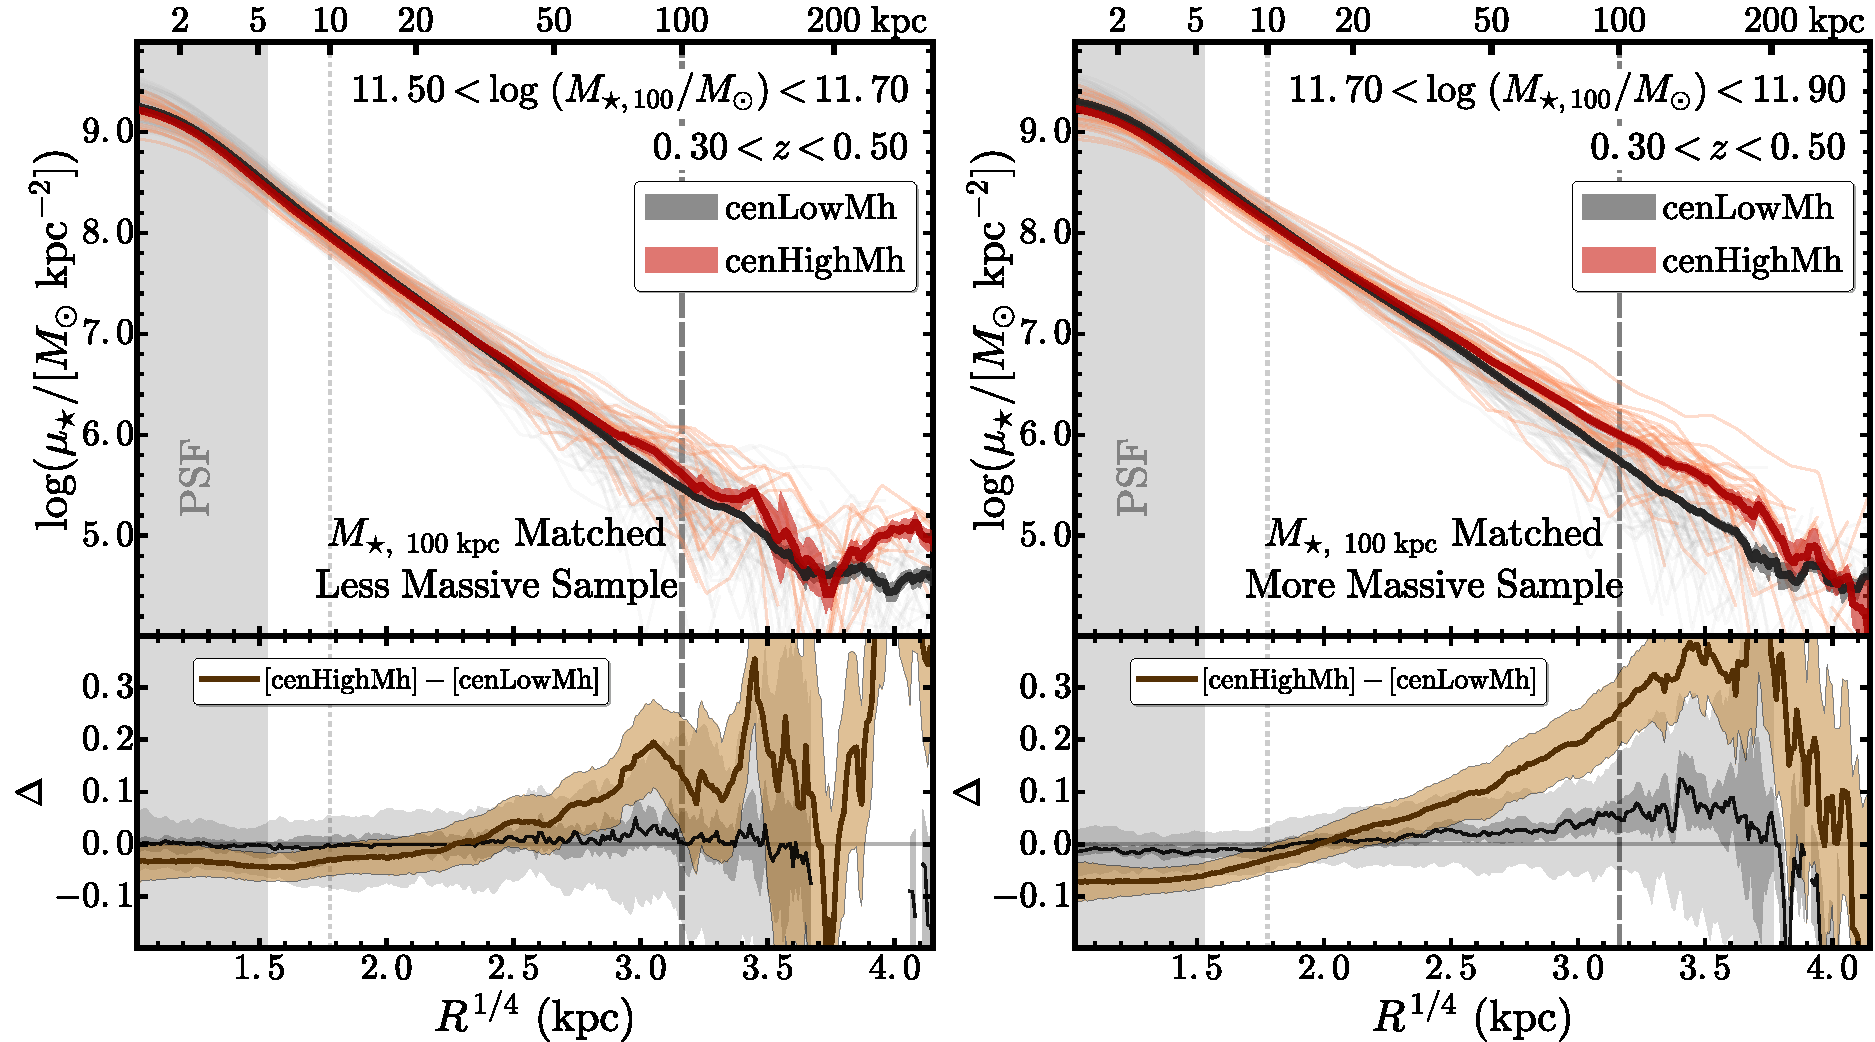
\includegraphics[width=\textwidth]{fig/redbcg_prof_2}
      \caption{Comparisons of the \mden{} profiles for \mtot{}-matched \rbcg{} 
          (orange-red) and \nbcg{} (grey-black) galaxies in lower (left; [11.5,11.70]) 
          and higher (right; [11.7, 11.9]) \mtot{} bins. 
          Other formats are in consistent with the right figure of Fig.\ref{fig:prof_1}.
          The difference in median profiles is more significant in higher \mtot{} bin.}
      \label{fig:prof_2}
  \end{figure*}
%% ------------------------------------------------------------------------------------ %% 

    \citet{Patel2013} extracted the median \mden{} profile of massive ETGs in a similar 
    redshift range with this work ($0.25 < z < 0.50$) using the stacked \textit{HST}/ACS
    images. 
    These galaxies are selected at a constant cumulative number density that makes them  
    good candidates of progenitors of $z=0$ massive ETGs.  
    The median \mstar{} is $\sim 10^{11.2} M_{\odot}$ according to their estimates.  
    However, given the shallower depth of the ACS images and the usage of the BC03 model 
    (each could cause -0.1 dex mass offset compared to this work), this sample should be 
    comparable to the galaxies in the lowest \mtot{} bin, and the comparison of their 
    median profiles does reflect that.  
    Moreover, the superb resolution of the \textit{HST}/ACS image makes the \mden{} 
    profile unaffected by PSF even within inner 1 kpc, hence the comparison illustrates 
    that the HSC profiles within our redshift range are indeed not bothered by 
    seeing outside the shaded region, and \minn{} should be very reliable.
    In fact, even \mstar{} within 5 kpc should be available for comparison.  
  
    Besides these observations, we also compare with the predicted average \mden{} 
    profile of central galaxies in very massive halos 
    ($13.5 < \log M_{200,c} < 14.0$) from cosmological simulation (\citealt{Cooper13}). 
    This is achieved by combining the detailed assembly information of halos from the 
    dark-matter-only simulation with semi-analytic model and particle-tagging technique 
    (\citealt{Cooper10}).
    Although the physical resolution and detailed baryonic processes are not as 
    ``realistic'' as state-of-art hydro-simulation, it is very efficient in providing 
    rough stellar mass distributions in a large sample of massive halos. 
    Without any adjustment, the profile is already quite similar to the median \mden{}
    profile of galaxies in the $11.6 <$\logmtot{}$< 11.8$ bin within 30-40 kpc. 
    But the simulation seems to predict too significant envelope at larger radius for 
    this average halo mass. 
    Although we will not dig into the detailed causes of such differences, it already 
    highlights that the comparison between deep \mden{} profiles from observations 
    and the predicted ones in simulations can be very interesting, especially in the 
    outskirt that was rarely discussed using previous data. 
    
    We summarize the median profiles in Fig.\ref{fig:avg_prof} in Table.~1,
    and all the above median profiles are available  
    \href{https://github.com/dr-guangtou/hsc_cenHighMh/tree/master/profiles}{here}.

%% ------------------------------------------------------------------------------------ %% 

\subsubsection{Environmental dependence of \mden{} profiles at fixed \mtot{}}
    \label{sssec:sbp_mtot}

    \update{
    We show the results of the comparison in Fig.\ref{fig:prof_1} after 
    carefully matching the \rbcg{} sample with smaller size to the \nbcg{} samples 
    within $0.3 < z < 0.5$ and $11.6 < $\logmtot{}$<11.9$ vial searching for the $N$ 
    nearest neighbours on the $M_{\star}$-redshift plane using the KDTree algorithm. 
    The details of the procedure and the evaluation of the matching quality can be 
    found in Appendix.\ref{app:match}. 
    In summary, given the typical uncertainty of stellar mass, the two samples are well 
    matched in \mtot{}; and their redshift distributions are broadly consistent with 
    each other, hence we can perform meaning comparison of their average structures at 
    ``fixed stellar mass'' (median \logmtot{}$\sim 11.74$).    
    We also check their distributions of $k$-corrected colors ($g-r$), and confirm 
    that they have similar color distributions as well.}
    
    For the 45 \rbcg{} galaxies, we have 229 unique \nbcg{} galaxies in the 
    matched sample.
    \update{
    On the left side of Fig.\ref{fig:prof_1}, we plot the individual \mden{} profile 
    of \rbcg{} and \nbcg{} galaxies along with the median profiles of both samples.
    The uncertainties of the median profiles are derived using 5000 times of 
    bootstrap resampling.
    The \mden{} profile out to such large radius was only available for large sample of 
    massive galaxies through image stacking method (e.g. \citep{Tal2011, DSouza2015}) 
    which suffers from certain systematic issues.}
    Although the \mden{} profiles of many galaxies extend well beyond the 100 kpc radius, 
    we notice that some profiles show sign of unphysical truncation that is caused 
    by inaccurate background subtraction.  
    Therefore, we will not include profiles outside 100 kpc in the comparison, even 
    though the median profiles within 200 kpc still behave normally.  
        
    Once we match the distributions of \mtot{}, the \mden{} profiles of massive 
    galaxies in the \rbcg{} and \nbcg{} samples \textbf{greatly overlap with each 
    other over the entire radius range}. 
    At fixed ``total'' stellar mass, massive central galaxies in more massive 
    halos do not form a unique population comparing to the ones from less massive 
    halos in term of their radial \mstar{} distributions. 
    \update{
    This partially explains why the previous works have trouble finding any clear 
    environmental dependence of structure.} 
    
    At the same time, thanks to the high-quality individual profile from HSC image, 
    we can also spot interesting differences in the median profiles of the 
    \mtot{}-matched \rbcg{} and \nbcg{} samples.  
    In details, it seems that the central galaxies in more massive halos tend to 
    have slightly flattened inner \mden{} profiles while also possess more significant 
    outer stellar envelope.   
    To highlight such subtle structural features, we show the difference between 
    the two median profiles and its uncertainty in the bottom panel. 
    Given the noticeable uncertainties of \mtot{} and $\lambda$, along with the 
    small size of the current \rbcg{} sample, we perform statistical test to confirm 
    the robustness of the result: we mix the $N_{\mathrm{r}}$ \rbcg{} galaxies and 
    the $N_{\mathrm{n}}$ \mtot{}-matched \nbcg{} ones together, then randomly draw 
    $N_{\mathrm{r}}$ galaxies with putting-back, compute the difference between the 
    median profile of this sample and the \nbcg{} sample. 
    \update{
    After repeating this process 2000 times, we can evaluate the possibility that 
    the systematic differences in median \mden{} profiles can be reproduced by random 
    selection of massive galaxies.
    Comparing with the statistical distributions of the differential profiles from 
    this test (grey shaded region), we can now conclude that the structural 
    differences between \rbcg{} and \nbcg{} samples are significant.}
    Apparently, the ``transition radius'' where the median profiles of \rbcg{} 
    and \nbcg{} sample have the same \mden{} is $\sim 15$-20 kpc, which is quite 
    close to the expected $R_{\mathrm{e}}$ of ETGs at this \mtot{} (please see 
    next section for details).
       
    To further test the robustness of this interesting result, we apply the above 
    procedures to \mtot{}-matched samples with slightly different definitions.  
    The results are shown in Fig.\ref{fig:prof_3} in Appendix.\ref{app:robust}: 
    (a). At higher redshift, the profile is affected more by the seeing at inner 
    region, and by the imaging depth in the outskirt.  
    Therefore, we compare the matched \rbcg{} and \nbcg{} samples within 
    $0.3 \leq z < 0.4$, and the results are very similar.
    (b). We also make the comparison using a \rbcg{} sample with lower average 
    halo mass ($\lambda \geq 20$), the results are still stable (middle panel). 
    We also check whether the structural differences are driven by small fraction 
    of \rbcg{} galaxies in very massive clusters.  
    After removing the \rbcg{} galaxies in clusters with $\lambda \geq 40$, the 
    differences are as significant as above.  
    (c). As noted before, the \mtot{} is just a proxy of the total stellar mass. 
    Given the differences we find, at fixed \mtot{}, \rbcg{} galaxy tends to have 
    slightly more prominent outer envelope outside 100 kpc than the \nbcg{} one. 
    Hence their real ``total'' stellar mass could also be slightly larger, and 
    bias the comparison.  
    Therefore, we make a similar comparison using the maximum \mstar{} from 
    the integration of the \mden{} profile instead of the \mtot{}.
    \update{
    In this case, the differences between the median profiles become slightly 
    less significant as expected (a fraction of \rbcg{} galaxies become more 
    massive, and is not included in the \logmtot{}$< 11.9$ mass bin). 
    But the systematic trends, especially the differences in the low mass density 
    outskirt are still very robust. 
    We will further discuss this in Section \ref{sec:discussion}. 
    Considering the uncertainty of \mden{} profiles outside 100 kpc, the 
    feasibility of applying the average \m2l{} to stars in the extreme outskirt, 
    and the contribution of the diffuse stellar components that trace the halo, 
    we think that our results are stable.}
    
    \textbf{All these tests confirm that we robustly detect subtle, but systematic 
    \mhalo{}-dependence (environmental dependence) of structure in massive, 
    central galaxies.}
    \update{
    Interestingly, the fact the it takes much better data and really cautious 
    comparison to detect such systematic difference seems to suggest that the role 
    played by environment in shaping the structure of central galaxies may not be 
    that crucial in the \mhalo{} and \mstar{} ranges we discussed.}
    
    At the same time, the systematic differences we find, especially the more 
    extended stellar envelope of massive central galaxy in more massive halos, 
    seem to be consistent with the expectation of richer (minor) merging history
    in denser environment. 
    \update{
    Predicted by the ``two-phase'' scenario, the non-dissipative mergers, especially 
    the minor ones, should mainly deposit stellar mass in the outskirts, help 
    build the stellar halo while do not change the inner \mden{} profiles very 
    much (e.g. \citealt{Hilz2013}, \citealt{Oogi2013}).}

    We also explore the possible \mtot{} dependence of such difference.  
    Limited by the small sample we have, we can only afford to separate the 
    samples into two \mtot{} bins, and extend to slightly lower \mtot{} bound 
    ($11.5 \leq \log (M_{\star,\ 10\mathrm{kpc}}/M_{\odot}) < 11.7$ and 
     $11.7 \leq \log (M_{\star,\ 10\mathrm{kpc}}/M_{\odot}) < 11.9$).  
    After performing the same procedures of sample matching and comparison, 
    we show the results in Fig.\ref{fig:prof_2}.   
    Although the smaller sample leads to larger statistical uncertainties, 
    it is still interesting to see that the structural differences seem to 
    be more significant in the higher \mtot{} bin.  
    For the lower \mtot{} bin, the difference in the inner region becomes quite 
    uncertain, while there is still evidence of difference in the outskirt.  
    This result also has interesting implications in the assembly history
    of massive galaxies, and is worth more investigations with larger samples
    in the near future.  

%% ------------------------------------------------------------------------------------ %% 

\subsubsection{Environmental dependence of \mden{} profiles at fixed \minn{}}
    \label{sssec:sbp_minn}

    \update{Here, we compare the median \mden{} profiles of \rbcg{} and \nbcg{} galaxies
    after matching the two samples using \minn{} ($11.2 <$\logminn{}$ < 11.6$) and 
    redshift ($0.3 < z < 0.5$).
    We use the same matching procedure as in the previous section, and also put its 
    evaluation in Appendix.\ref{app:match}.
    As mentioned in the beginning, here we use \minn{} as the proxy of the 
    \mstar{} of the ``in-situ'' component. 
    We will discuss this assumption more in the Section~\ref{sec:discussion}, but 
    observations and simulations seem to support this claim in general. 
    In the previous section, we investigate the environmental dependence of structure 
    using ``total'' \mstar{}; here, we compare the massive galaxies in low- and 
    high-mass halos that share similar amount of ``in-situ'' component.}
    
    \update{
    As we can see in Fig.\ref{fig:prof_1} and the Appendix.\ref{app:D}, the \minn{} is 
    not affected by the physical size of PSF out to $z=0.5$.  
    For the 56 galaxies in this \rbcg{} sample, we achieve excellent matching 
    result using 375 \nbcg{} galaxies (see Fig.\ref{fig:match}; 
    median \logminn{}$\sim 11.35$).  
    Using the same method, we show their individual profiles, and the comparison of 
    their median \mden{} profiles on the right side of Fig.\ref{fig:prof_1}.}
    
    Unlike the \mtot{} matched samples, here we see very striking differences that 
    are already very significant even without any statistical test.     
    \update{
    It is easy to see that, when matched at the same \minn{}, the \mden{} profiles of 
    \rbcg{} and \nbcg{} galaxies are quite similar in the inner 5-10 kpc.
    However, outside inner 10-15 kpc, the \rbcg{} galaxies show much more prominent
    stellar envelope.}     
    Besides the differences in the median profiles, it is also worth discussing 
    the distributions of individual \mden{} profiles. 
    \update{
    Combining the \rbcg{} and \nbcg{} samples together, we should notice that 
    the slope of the \mden{} profile inside 10 kpc is quite uniform, and the dynamic 
    range of the \mden{} values is pretty small. 
    On the other hand, the outer \mden{} profiles of massive central galaxies 
    can have a larger range of slopes. 
    The ones from more massive halos on average have shallower outer \mden{} 
    profiles, which is in qualitative agreement with recent simulation results 
    (e.g. \citealt{Pillepich2014}).
    And, for both \rbcg{} and \nbcg{} samples, we find their outer profiles 
    clearly have much larger dynamic range of \mden{} values at fixed radius.
    This interesting diversity is also clearly illustrated by 
    Fig.\ref{fig:m100_m10_color}, where we show the 3-color images of randomly 
    selected massive central galaxies that have similar \minn{} 
    ($11.1 \leq \log (M_{\star,\ 10\mathrm{kpc}}/M_{\odot}) < 11.2$)
    but different \mtot{}.   
    From the top-left to the bottom-right, the \mtot{} of these galaxies increases
    from $10^{11.22} M_{\odot}$ to $10^{11.75} M_{\odot}$.}
    
    \update{
    Putting together, these results indicate that massive central galaxies with 
    similar \mstar{} in the ``in-situ'' components share very similar radial 
    \mstar{} distributions in the inner region. 
    Given the highly dissipative nature of the ``in-situ'' phase, this is consistent
    with the prediction that dissipative process like intense star-formation or 
    wet-merger should create de~Vaucouleur-like ($n\sim 4$) \mden{} profile
    (e.g. \citealt{Hopkins2008}).
    On the other hand, the outer envelope of massive galaxies should be slowly 
    assembled through non-dissipative accretion process, where merger history 
    should play a essential role.  
    Therefore, it is reasonable to see that the central galaxy of more massive 
    halo has more significant stellar envelope than the one from lower mass 
    halo at fixed \mstar{} of their ``in-situ'' components.
    }
    
    \update{
    Despite that the structural contrast is very clear using the median \mden{} 
    profile, we still perform a serious of tests to verify the robustness of the 
    results. 
    Changing the redshift range or the lower $\lambda$ bound of the \rbcg{} sample 
    has no impact in the significance of the results; 
    Replacing the \minn{} with the \mstar{} within 5 or 15 kpc will result in 
    very similar differences; 
    And, unlike the \mtot{}-matched samples, spitting the samples into two \minn{} 
    bins (above and below \logminn{}$=11.4$) reveals no apparent \minn{}-dependence 
    of the structural differences.
    During the comparison, we notice that there is still tiny structural difference
    within 10 kpc (right figure of Fig.\ref{fig:prof_1}).
    When we match the two samples using both \minn{} and \meff{}, we notice that 
    inner median \mden{} profiles within 10 kpc becomes extremely similar 
    (see Fig.\ref{fig:match} in Appendix.\ref{app:match}), while the differences 
    in the outer part remain the same. 
    Hence, for \rbcg{} and \nbcg{} galaxies that share not only the same inner mass, 
    but also the same inner \mden{} profiles, we still see significant environmental 
    dependence in their overall structure.}
    
    \update{
    When we match the two samples using \minn{}, the matched samples have 
    different \mtot{} distributions (median \logmtot{}$\sim 11.78$; 
    median \logmtot{}$\sim 11.64$).  
    Although it is still safe to say that they represent very massive central 
    galaxies, we also notice that the \nbcg{} sample starts to include galaxies with 
    $11.2 \leq$\logmtot{}$< 11.6$. 
    For one thing, our samples start to become quite incomplete below 
    \logmtot{}$\sim 11.5$-11.6; the satellite contamination could also increases
    toward lower \mtot{} end.  
    More importantly, when the \mtot{} becomes very different, it is no longer 
    comfortable to assume that they can share very similar ``in-situ'' components 
    even at the same \minn{}, as they could be in different phases of evolution.
    Therefore, we also match the two samples using \minn{} again, but only include the 
    massive ones with \logmtot{}$\geq 11.5$.  
    Comparison between these more complete, purer samples of massive central galaxies 
    shows very similar structural differences again (see the right side of 
    Fig.\ref{fig:match} in Appendix.\ref{app:match}).
    In fact, their median profiles become even more similar in the inner region,
    suggesting that the results are very robust.}
    
    \update{
    The median profiles shown in Fig.\ref{fig:prof_1} are available in 
    Table.1.}

%% ------------------------------------------------------------------------------------ %% 

\subsection{Comparisons of ellipticity and optical-color profiles}
    \label{ssec:ell_color}
    
%% ------------------------------------------------------------------------------------ %% 
  \begin{figure*}[t!]
      \centering 
      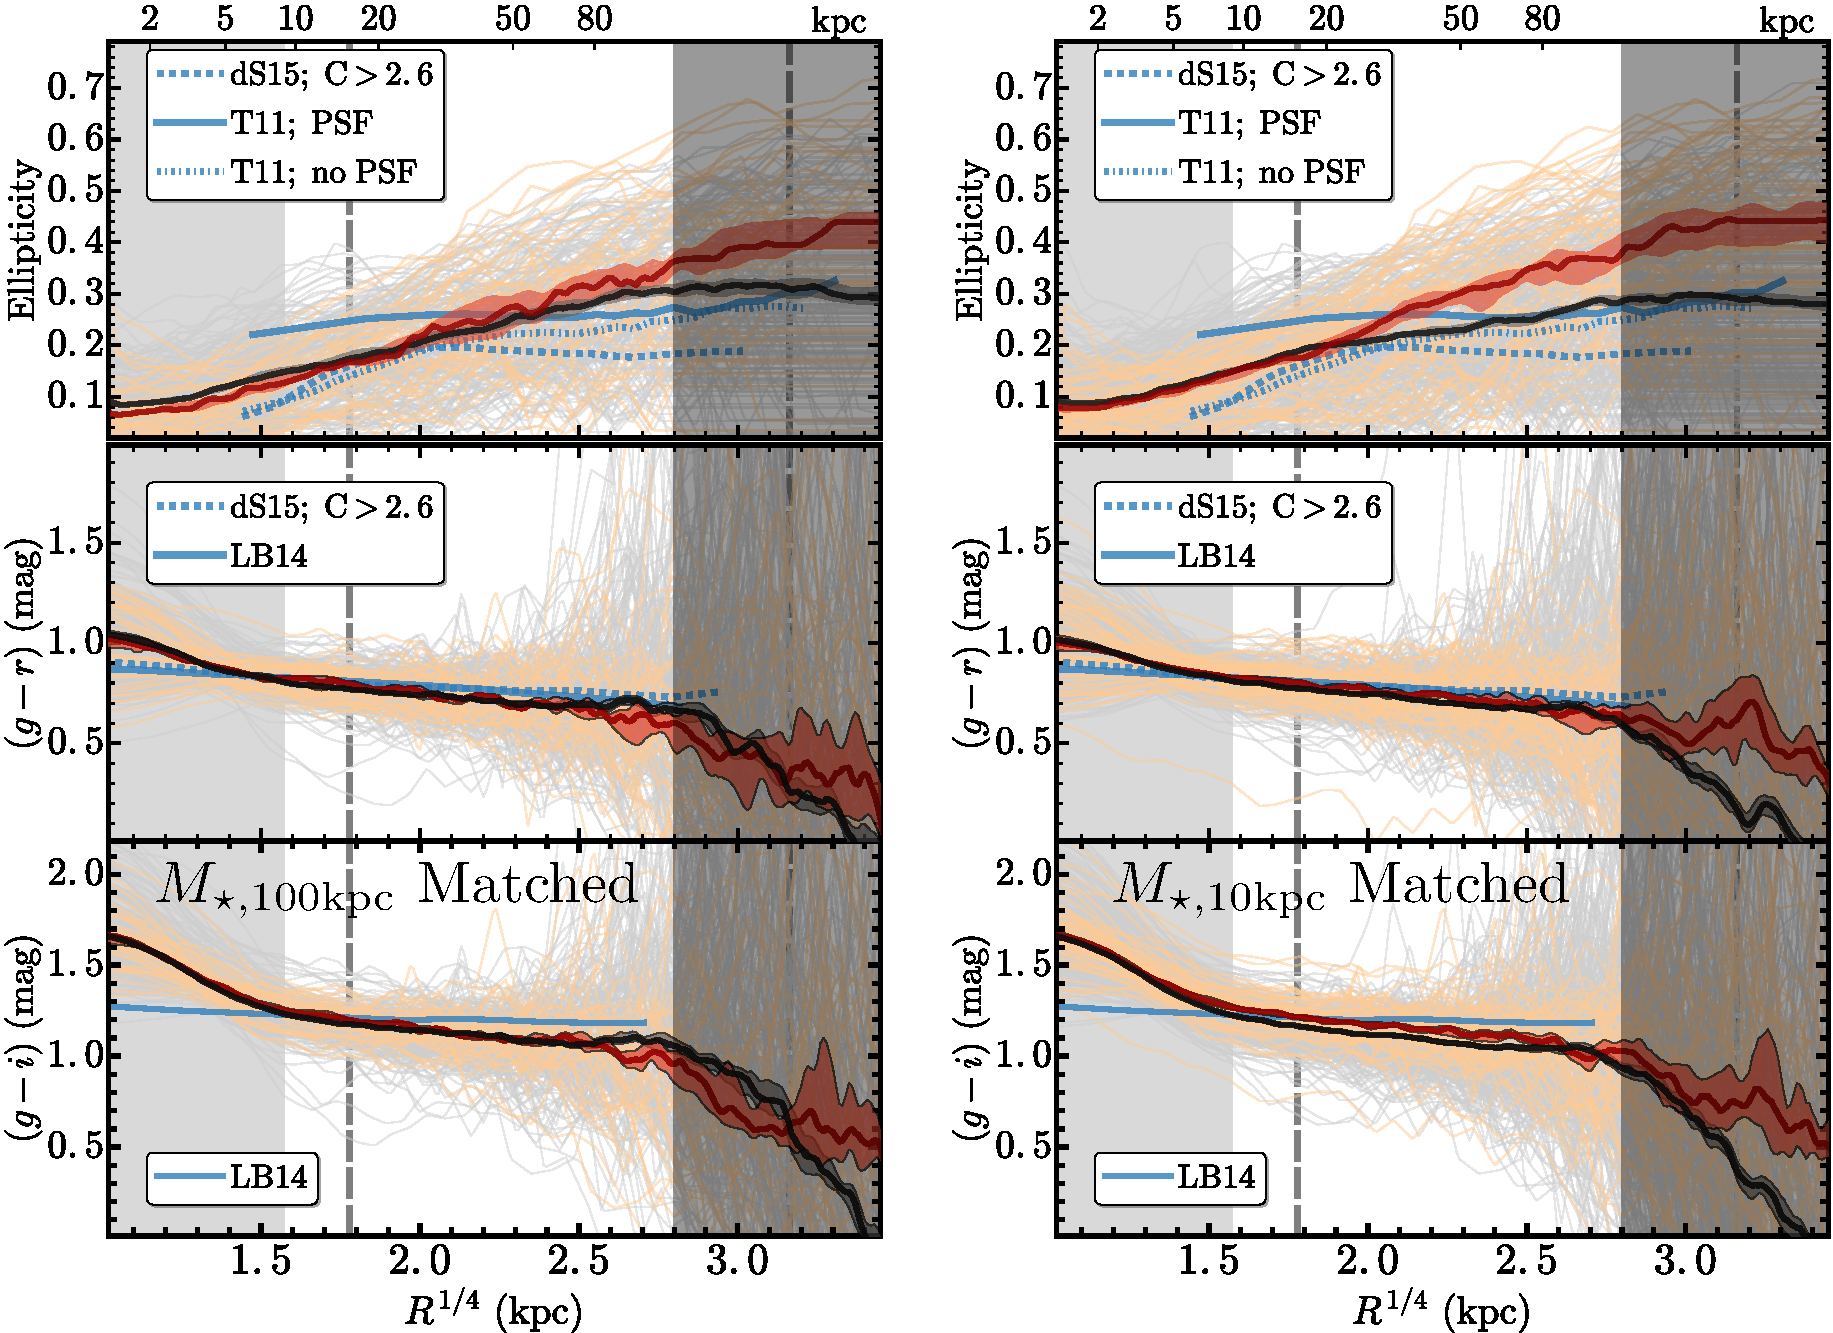
\includegraphics[width=\textwidth]{fig/redbcg_discussion_2}
      \caption{Comparisons of the radial profiles for ellipticity and optical colors 
      	for \mtot{}-matched (\textbf{left figure}) and \minn{}-matched 
      	(\textbf{right figure}) of \rbcg{} (orange-red) and \nbcg{} (grey-black) samples. 
        The formats are very similar to the figure for \mden{} profile 
        (e.g. right figure of Fig.\ref{fig:prof_1}). 
        On each side, from top to bottom, we show the elliptical profile, and the 
        color profile using $g-r$ and $g-i$ color. 
        Since the individual profile of these properties has very large uncertain in the 
        outskirt, we block the region at large radii where we think the median profiles 
        are still unreliable using a dark, shaded box.
        We also compare these results with previous results based on SDSS images. 
        They are: 
        1) Ellipticity profile of the stacked image of a large sample of red galaxies at 
        $z\sim 0.4$ from \citet{Tal2011} with PSF correction 
        (solid blue line on top panel); 
        2) Ellipticity and $g-r$ color profiles from stacking analysis of nearby massive 
        galaxies with high concentration index ($C>2.6$) in \citet[][blue dash lines 
        on the top and middle panels]{DSouza2014}; 
        3) average $g-r$ and $g-i$ color profiles for a large sample of nearby 
        elliptical galaxies in \citet[][blue, solid lines on the middle and bottom 
        panels]{LaBarbera2010}.}
      \label{fig:ell_color}
  \end{figure*}
%% ------------------------------------------------------------------------------------ %% 
    
    \update{
    In the above section, we focus on the 1-D \mden{} profiles that are based on 
    $i$-band image along. 
    Although they already help us reveal interesting structural differences, we 
    should not forget that the multi-band, 2-D HSC images of massive galaxies 
    contain more information. 
    Among them, the shapes and colors of different stellar components are particularly 
    important to look into.
    Here, we extract the radial profiles of ellipticity and $k$-corrected optical colors
    of galaxies in both \mtot{}-matched and \minn{}-matched samples (used in 
    Fig.\ref{fig:prof_1}) using \texttt{Ellipse}, and compare the average profiles between
    the \rbcg{} and \nbcg{} samples for two main purposes:}
    
    \begin{enumerate}
        \item \update{Since we derive the \mden{} profiles using average isophotal 
            shape, if these massive galaxies have steep or complicated elliptical 
            profiles, or the two samples share very different elliptical profiles, 
            the comparison of the average \mden{} profiles could be biased.
            Therefore, we want to verify that photometry using average isophotal 
            shape is appropriate for these samples. 
            We extract ellipticity profiles in $i$-band using \texttt{Ellipse} by 
            setting the geometric parameters free while forcing all isophotes share 
            the same center.}
        \item \update{As emphasized earlier, we apply the average \m2l{} to derive 
            \mstar{} of these massive galaxies knowing that the \m2l{} changes with 
            radius.  Although this may not be a critical issue when deriving ``total''
            \mstar{}, it certainly can bias the comparisons of \mden{} profiles when 
            two samples have very different \m2l{} profiles. 
            So we want to confirm that the application of average \m2l{} is reasonable
            using the optical color profiles as tracer of \m2l{}.  
            After preparing the images in other bands in the same way with $i$-band 
            ones, we derive color profiles by applying the isophotes from $i$-band 
            to other images in a ``forced photometry'' mode.}
    \end{enumerate}

    \update{
    Strictly speaking, we need better background subtraction and 2-D modeling method 
    to accurately recover these information. 
    But the straightforward methods applied here are sufficient for these purposes. 
    We make no correction to the differences in background subtraction and PSF in 
    different bands, therefore, we will simply ignore the shape and color information 
    in the inner-most region and very low surface brightness regime. 
    The profiles between 5-50 kpc should be useful. 
    Here we only consider $g$ and $r$ band data as the ones in $z$ and Y-band are 
    often shallower, have worse seeing, and suffer more from background subtraction 
    issues. 
    We apply Galactic extinction and $k$-correction to both $g-r$ and $g-i$ color 
    profiles; the $k$-correction values are also from \texttt{iSEDFit} results.
    We show the average ellipticity, $g-r$, and $g-i$ color profiles for the 
    \mtot{}-matched (\minn{}-matched) samples of \rbcg{} and \nbcg{} galaxies on the 
    left (right) side of \ref{fig:ell_color}, and also compare them with previous 
    estimates that are based on stacking analysis of SDSS galaxies 
    (e.g. \citealt{LaBarbera2010, Tal2011, DSouza2014}).}
    
    \update{
    Firstly, it is easy to see that massive central galaxies on average have positive 
    ellipticity profiles. 
    The ellipticity slowly, but steadily increase with radius from $e\le 0.2$ around 
    5-10 kpc to $e\sim 0.3$ at 40-50 kpc.  
    For the \mtot{}-matched samples, their ellipticity profiles trace each other 
    very well all the way to 50 kpc (2-3$\times R_{\mathrm{e}}$ for their \mstar{}); 
    there might be hints that the \rbcg{} ones have higher ellipticity at larger 
    radius, but the isophotal fits with free geometry become very unstable at such 
    low surface brightness region. 
    This confirms that the comparisons of \mden{} profiles using average isophotal 
    shape is reasonable. 
    On the other hands, when matched using \minn{}, the \rbcg{} galaxies show 
    systematically higher ellipticity than the \ncbg{} ones at $r > 10$ kpc, despite 
    the ellipticity profiles at inner region are still very similar. 
    Since the average ellipticity value is still quite low, and the slope of the 
    profile is very shallow, the differences in ellipticity profiles will not affect 
    the significant differences in \mden{} profiles. 
    And it further hints different assembly histories of the outer envelopes of
    central galaxies in different environments. 
    These results are in consistent with the ones from 2-D decomposition in
    \citep{Huang2013a}: the outer envelopes of massive ETGs have higher ellipticity 
    than the inner, ``in-situ'' dominated region; and become more elongated with 
    \mstar{}. 
    As for the ellipticity profile, although it contains interesting information 
    regarding the assembly history, it is difficult to estimate them down to very 
    large radius. 
    \citet{Tal2011} stacked the SDSS images of a large sample of Luminous Red 
    Galaxies (LRGs) at $z\sim 0.4$, and extract the ellipticity profile after 
    correcting the PSF convolution effect.   
    Its slope is much shallower than the average ones using HSC images, despite the 
    two samples are at similar redshift and are quite comparable. 
    The poorer seeing condition of SDSS image plus the systematics in the stacking 
    process can easily explain this. 
    \citet{DSouza2015} performed similar stacking analysis for a large sample of very 
    nearby ETGs.  
    The ellipticity profile is quite consistent with our average ones within 5-10 
    kpc, but become much shallower at outer region.  
    The lower average \mstar{} of their sample and/or the uncertainties in the 
    stacking analysis may explain this.  
    This highlights the advantages of the high-resolution, deep HSC images again,
    and it would be very interesting to compare with numerical simulations. 
    }
    
    \update{ 
    Secondly, we see shallow and negative gradients of average $g-r$ and $g-i$ color 
    profiles for both \rbcg{} and \nbcg{} galaxies after excluding the unreliable 
    regions. 
    On the left of Fig.\ref{fig:ell_color}, we see that the \rbcg{} and \nbcg{} 
    samples share very similar color profiles from 5-50 kpc. 
    This is very good news for using average \m2l{} in the comparisons of \mden{}
    profiles: although the \mden{} profiles may not be perfectly accurate, there 
    should be no bias when comparing the average profiles of \rbcg{} and \nbcg{} 
    samples.
    On the right side of Fig.\ref{fig:ell_color}, the situation is very similar 
    as the slopes of color gradients are basically the same for two samples; 
    although there might be some evidence that, when matched at similar \mstar{} 
    of the ``in-situ'' component, the \rbcg{} galaxies tend to have slightly redder
    envelopes than the \nbcg{} ones. 
    This is worth further investigation, especially vial multi-band, 2-D 
    decomposition method. 
    Ignoring the tiny differences between the corresponding HSC and SDSS filters, 
    we see quite consistent $g-r$ color profiles; but the $g-i$ profiles become 
    slightly steeper using HSC images. 
    Although the exact cause of this difference is not clear, it is worth noting that
    the SDSS $i$-band images suffer from the ``red-halo'' effect of extended PSF 
    wing (e.g. \citealt{Wu2005}, \citealt{Tal2011}) which could make the color 
    at larger radius appear redder.
    Thank to the thickness of the CCD, the HSC $i$-band images do not have this 
    problem, hence can provide more accurate color estimates.
    }

    \update{
    Although the 1-D analysis is not perfect, these preliminary results already 
    point out the importance and benefits of including multiband, 2-D information 
    into account. 
    Now we know that, for massive central galaxies with similar \mtot{}, the average 
    \mden{} profiles show subtle dependence on halo mass, while the color and 
    ellipticity profiles are very stable.  
    On the other hands, for central galaxies that have the same \mstar{}, ellipticity 
    and color profiles within 10 kpc, their outer envelopes appears to be strongly 
    depend on environments. 
    }
    
%% ------------------------------------------------------------------------------------ %% 

\subsection{Explore Different Scaling Relations}
    \label{ssec:scaling}

%% ------------------------------------------------------------------------------------ %% 
  \begin{figure}[bt!]
      \centering 
      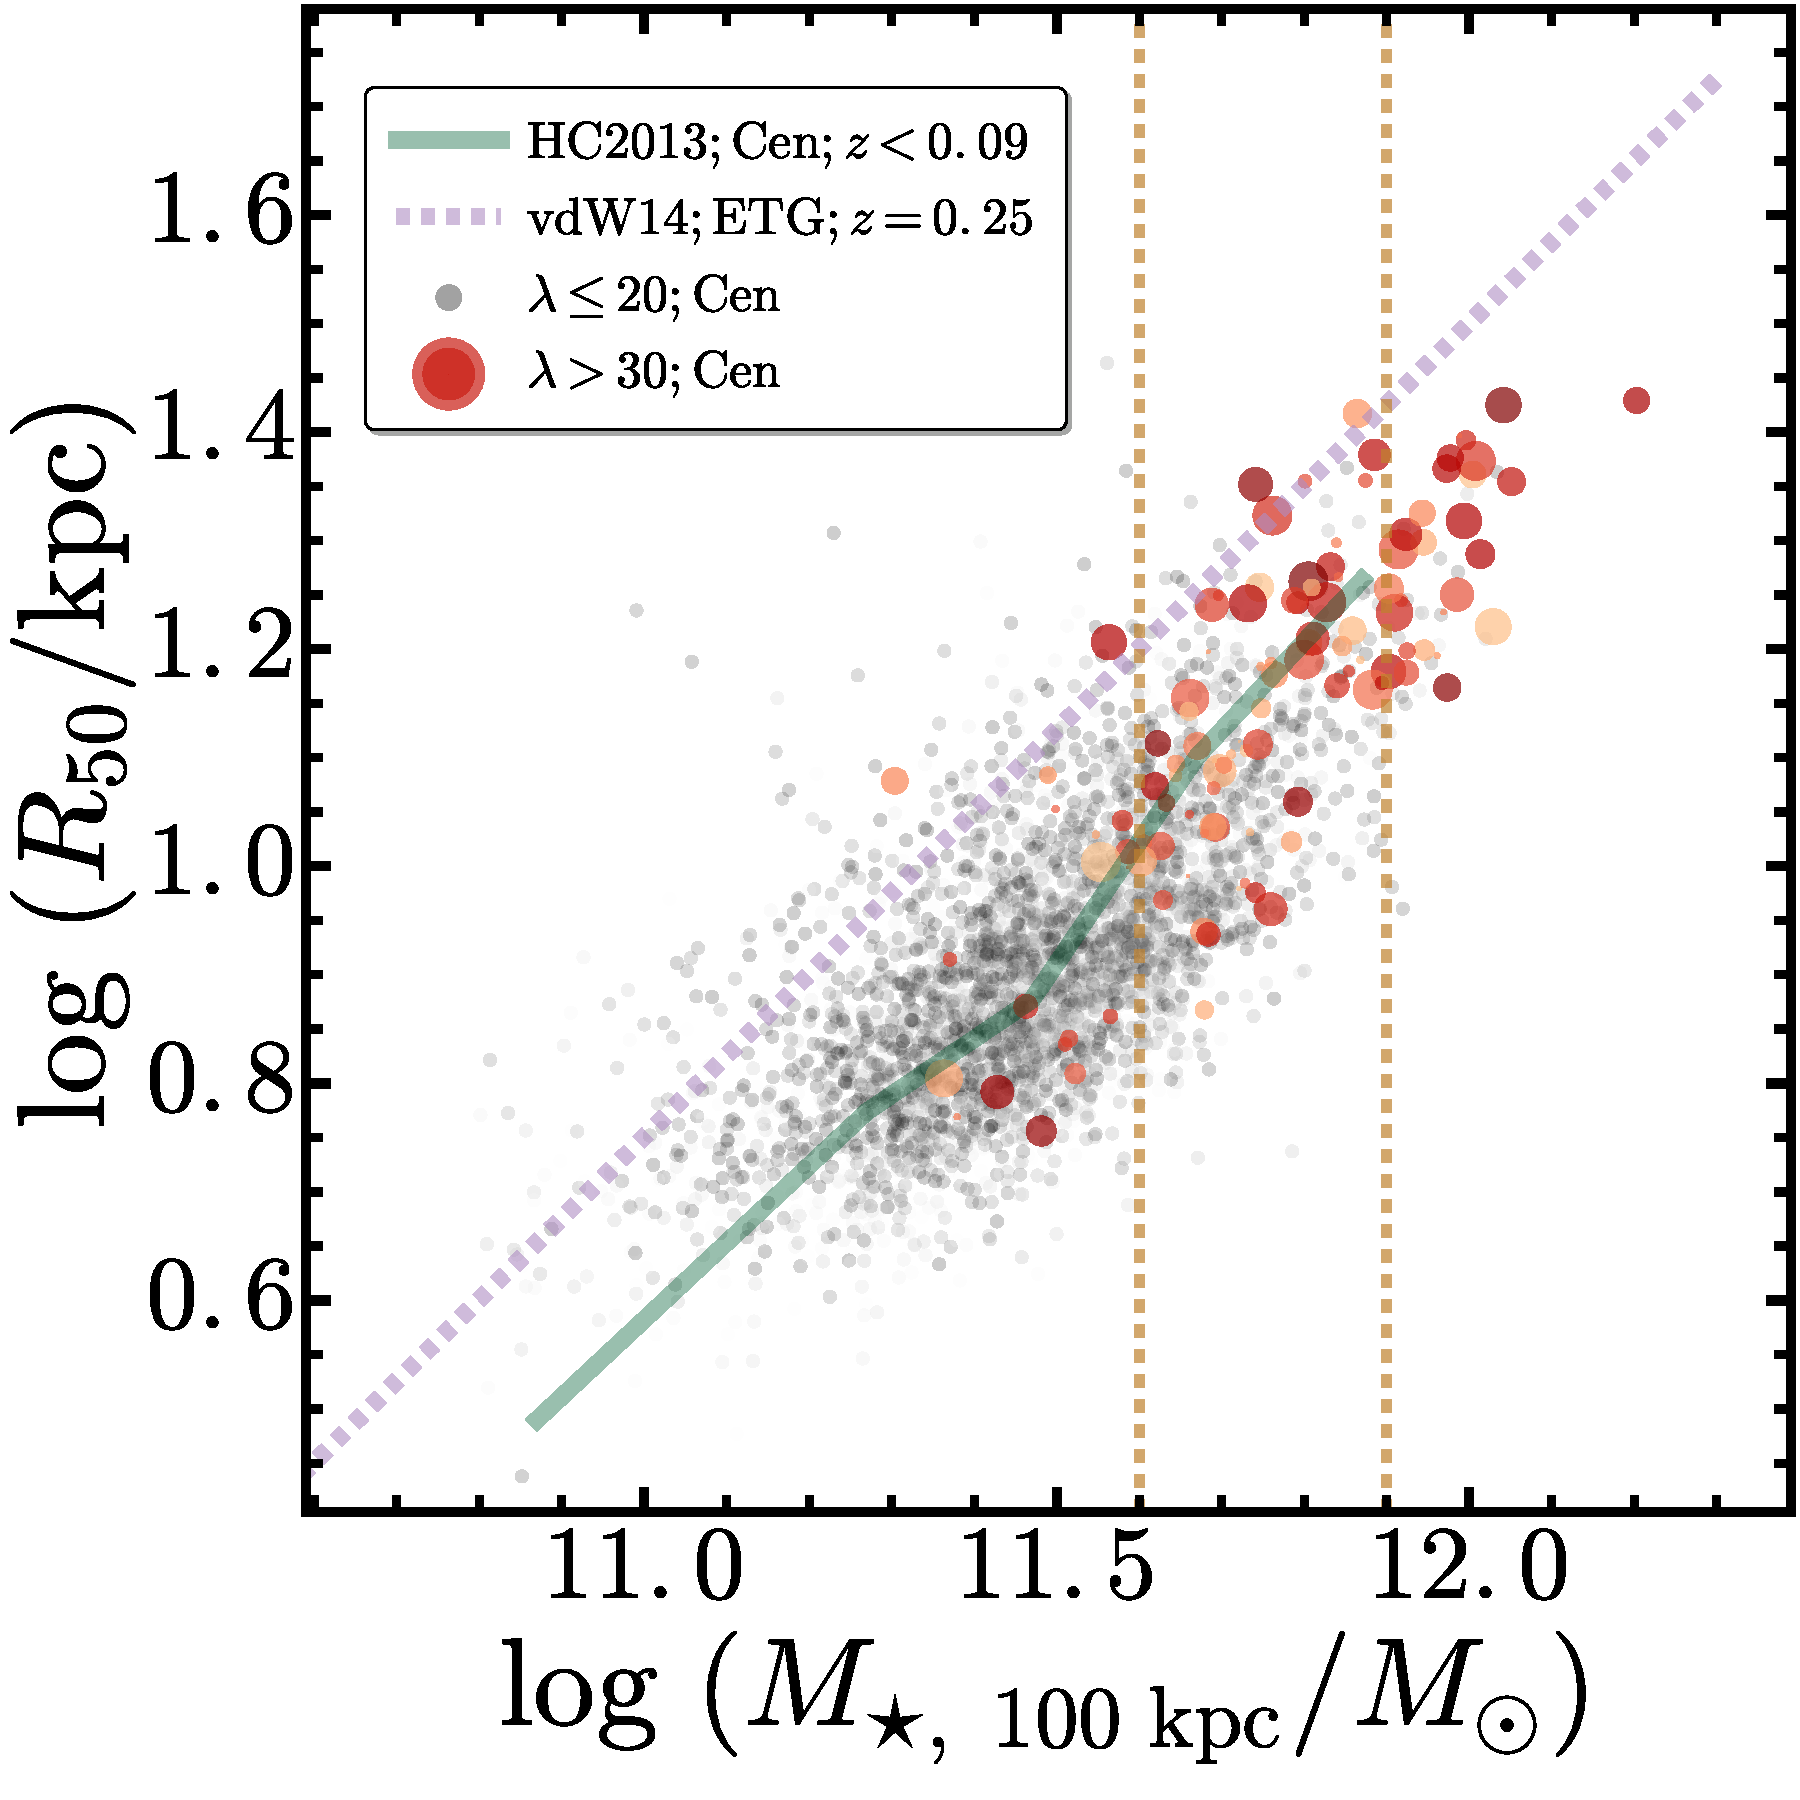
\includegraphics[width=\columnwidth]{fig/redbcg_mass_r50}
      \caption{The \mstar{}-size relations for \rbcg{} (orange-red circles) and \nbcg{} 
          (grey dots) galaxies. 
          Here we use the \mtot{} as proxy of total \mstar{}, and use the 
          $R_{\mathrm{50}}$ derived from the 1-D profile as size estimate. 
          Two vertical lines highlight the $11.6<$\logms{}$<11.9$ mass bin.
          We visualize the best-fit \mstar{}-$R_{\mathrm{50}}$ relations of \rbcg{} 
          (red, solid line) and \nbcg{} (grey, dash line) galaxies at high-\mstar{} end.
          The shaded regions in lighter colors show the 1-$\sigma$ uncertainties
          from MCMC sampling. 
          We also compare with the \mstar{}-$R_{\mathrm{50}}$ relation for nearby central 
          galaxies in massive groups from \citet{HCompany13} (green, long dashed line). 
          Please refer to the text for more details.}
      \label{fig:mass_r50}
  \end{figure}
%% ------------------------------------------------------------------------------------ %% 

\subsubsection{$M_{\ast}-$size relation}
    \label{sssec:mass_size}
        
    The scaling relation between \mstar{} and effective radius (or half-light radius;
    $R_{\mathrm{e}}$ or $R_{\mathrm{50}}$) 
    was the focus of previous investigations of the structural evolution 
    (e.g. \citealt{Shankar2013}; \citealt{Leja2013}, \citealt{vdWel2014}) and 
    the environmental dependence of structures for massive galaxies 
    (e.g. \citealt{Weinmann2009}, \citealt{Nair2010}, \citealt{HCompany13}, 
    \citealt{Cerbrian2014}). 
    So far, the results are quite confusing as no clear evidence of environmental 
    dependence has been found at low redshift using various definitions of ``size''. 
    And the observations become controversial at intermediate and high redshift
    (e.g. \citealt{MCooper2012}, \citealt{Papovich2012}, \citealt{Kelkar2015}).
    \update{
    Through careful comparisons of \mden{} profiles at fixed \mtot{} and \minn{}, 
    we clearly show that the structure of massive central galaxies at $0.3 < z < 0.5$
    depend on the halo mass in a subtle but systematic manner. 
    Therefore, we also expect to see such evidence on the \mstar{}-size relations 
    of \rbcg{} and \nbcg{} galaxies (see Fig.\ref{fig:mass_r50}).}
     
    We choose to use the \mtot{} as the proxy of ``total'' \mstar{}, and use the 
    radius that encloses 50\% of luminosity within 100 kpc ($R_{\mathrm{50}}$) as 
    the ``size'' to evaluate the relation.
    We use the curve-of-growth of luminosity from the \texttt{Ellipse} run on 
    $i$-band images to estimate the $R_{\mathrm{50}}$ here.
    This 1-D approach is more sensitive to issues like the smearing effect of PSF and 
    the choice of aperture for maximum luminosity than the 2-D fitting method.
    But, for the massive galaxies in this work, their apparent sizes are always 
    sufficiently large at $0.3 \geq z \geq 0.5$ so that the $R_{\mathrm{50}}$ 
    measurements are not bothered by seeing.  
    At the same time, this 1-D method has the advantages of being less affected by the 
    accuracy of background subtraction, structural details, and model assumptions.
    
    On Fig.\ref{fig:mass_r50}, we see clear \mstar{}-size relations for both samples.  
    At fixed \mtot{}, the distributions of $R_{\mathrm{50}}$ for the \rbcg{} and
    \nbcg{} galaxies greatly overlap.  
    Meanwhile, it seems that the \rbcg{} galaxies do have a slightly higher 
    $R_{\mathrm{50}}$. 
    For the \mtot{}-matched samples used in Fig.\ref{fig:prof_1}, the median 
    $\log (R_{\mathrm{50}}/\mathrm{kpc})$ values for the \rbcg{} and \nbcg{} are 
    $1.22\pm 0.02$ ($\sim 17.4\pm 0.75$ kpc) and $1.09\pm 0.01$ 
    ($\sim 12.3\pm0.3$ kpc), which confirm the above observation and is consistent with 
    the differences seen in Fig.\ref{fig:prof_1}. 
    However, most previous works that we are aware of did not match the \mstar{} 
    and redshift distributions between different samples, and often focused on the shape 
    of the \logms{}-$\log R_{\mathrm{e}}$ relation.  
    Here, we try to derive the best-fit parameters for the 
    \logmtot{}-$\log (R_{\mathrm{50}}/\mathrm{kpc})$ relations of galaxies with 
    \logmtot{}$\geq 11.6$ using MCMC-sampling method via the ensemble sampler 
    \texttt{emcee} (\citealt{Emcee}). 
    Using initial guesses based on maximum likelihood estimates, and assuming reasonable 
    flat priors, we derive best-fit relations for the massive \rbcg{} galaxies:
    
    \begin{equation}
        \begin{aligned}
        \log (R_{\mathrm{50}}/\mathrm{kpc}) = & (0.73\pm0.13) \times \log (M_{\star, 100\ \mathrm{kpc}}/M_{\odot}) \\ & -(7.49\pm1.56)
        \end{aligned}
    \end{equation}

    \noindent And for the massive \nbcg{} galaxies, we have:
    
    \begin{equation}
        \begin{aligned}
        \log (R_{\mathrm{50}}/\mathrm{kpc}) = & (0.68\pm0.06) \times \log (M_{\star, 100\ \mathrm{kpc}}/M_{\odot}) \\ & -(6.88\pm0.75)
        \end{aligned}
    \end{equation}
    
    \noindent As shown in Fig.\ref{fig:mass_r50}, at the high-mass end, the two relations 
    have consistent slopes within their uncertainties, but different normalizations. 
    Extending the fitting to the full \logmtot{} range does not change this result. 
    We also explore mass-size relations for our samples using \mstar{} within different 
    radius (e.g. 120, 150 kpc) and the $R_{\mathrm{50}}$ derived within these apertures, 
    and find consistent results.
    
    We qualitatively compare our results with the one for $z\leq 0.09$ central ETGs in  
    $14\le$\logmh{}$<15$ halos from \citealt{HCompany13} (HC13; green solid line).
    HSC13 used the group catalog by \citet{Yang2007} to estimate \logmh{}. 
    They estimated the 2-D $R_{\mathrm{e}}$ using single-\ser{} model fitting to SDSS 
    images, and derived \mstar{} based on SED fitting using the BC03 (\citealt{BC03}) 
    synthetic population model.
    We empirically convert their \mstar{} from the Kroupa IMF to the Chabrier one 
    used in this work by applying a constant -0.05 shift to their values (see 
    \citealt{Bernardi2016}). 
    We also increase the \mstar{} in HC13 by $+0.1$dex to account for the systematic 
    difference between their BC03 and our FSPS model (see Appendix.\ref{app:B}). 
    In HC13, the authors found no difference among the mass-size distributions for 
    central galaxies in halos across $12.5\le$\logmh{}$<15.0$. 
    Despite all the systematic differences, the mass-size distributions for both \rbcg{} 
    and \nbcg{} galaxies follow the HC13 relation reasonably well (with slightly
    shallower slopes) even at \logmtot{}$< 11.6$ where our samples start to become 
    incomplete. 
    
    In short, we confirm that the massive central galaxies in this work generally 
    follow the \mstar{}-size relation for massive ETGs at low-$z$.
    \update{
    More importantly, we find that the \mstar{}-size relations at high-\mstar{} end 
    depends on \mhalo{}, suggesting that the central galaxies in denser environment 
    (higher \mhalo{}) have slightly larger $R_{\mathrm{50}}$ comparing to the 
    ones from smaller haloes at fixed \mtot{}. 
    }
    
    It would be interesting to revisit this topic using 2-D models based on deep HSC 
    images as the next step.
    It is worth noting that our results are based on massive galaxies at $z\sim 0.4$, 
    while the sample of HC13 has $z<0.09$.
    \update{
    Although here we can not study the redshift evolution of \mstar{}-size relation 
    here, it will be interesting to see whether the structural evolution of massive
    galaxies between $z\sim 0.4$ and $0.0$ also depends on environment. 
    If the \rbcg{} galaxies experienced more megers than the \nbcg{} ones during this 
    time, we should expect that \mstar{}-size relation shows stronger environmental 
    dependence at $z\sim 0.0$ using deeper image than SDSS.} 
    On the other hand, if the \nbcg{} galaxies could assemble more \mstar{} through
    minor mergers in the last 3-4 Gyrs, they could potentially ``catch-up'' with the 
    \rbcg{} galaxies on the \mstar{}-size plane, and makes it harder to find the 
    environmental dependence in nearby universe.
    In principle, we can make uses of the frequency of tidal features and the numbers 
    of satellites around our \rbcg{} and \nbcg{} galaxies to make some predictions 
    in the near future.
    
%% ------------------------------------------------------------------------------------ %% 

%% ------------------------------------------------------------------------------------ %% 
  \begin{figure*}[t]
      \centering 
      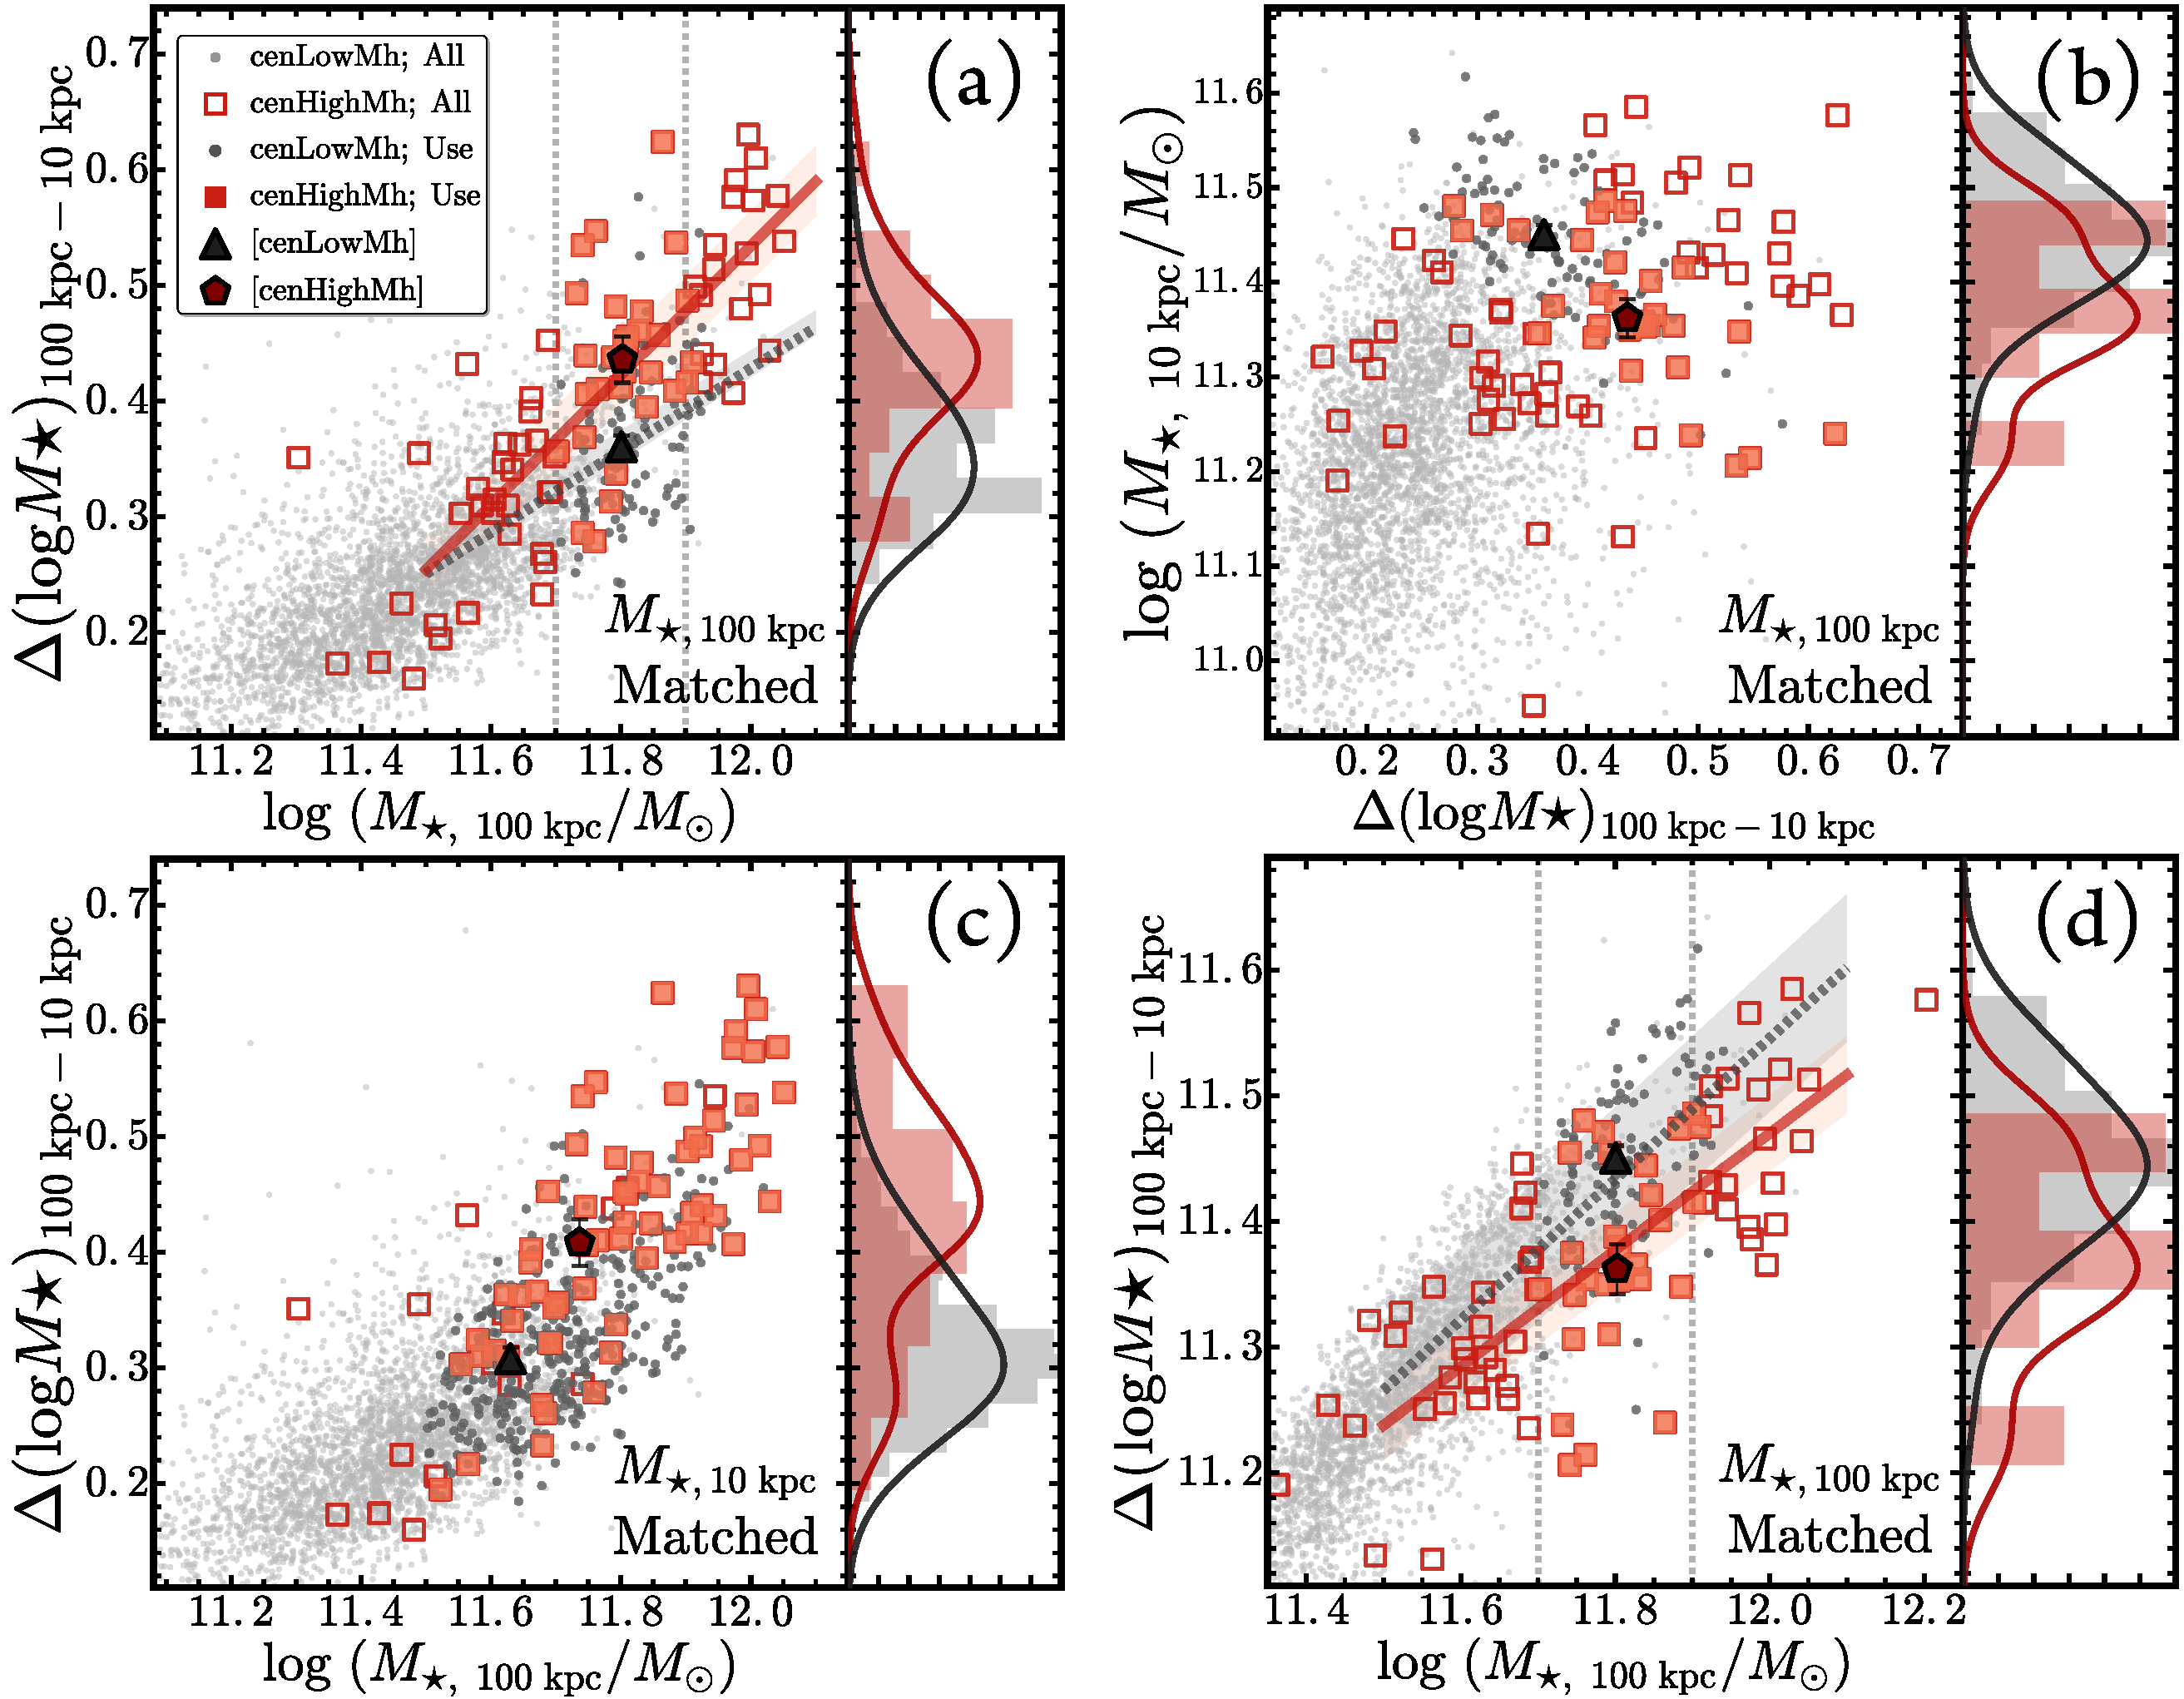
\includegraphics[width=\textwidth]{fig/redbcg_m100_m10_new}
      \caption{\textbf{(a)}: Distributions of galaxies on the 
          \mtot{}-$\Delta (\log M_{\star})_{100\mathrm{kpc}-10\mathrm{kpc}}$ plane. 
          All \rbcg{} (open red boxes) and \nbcg{} (light, grey dots) galaxies 
          are shown in the background. 
          The \mtot{}-matched samples between $11.6<$\logms{}$<11.9$ (between two 
          vertical lines) are highlighted (\rbcg{}: solid red boxes; 
          \nbcg{}: bigger grey dots). 
          We also show the median values (solid triangular and hexagon), and the
          distributions of $\Delta (\log M_{\star})_{100\mathrm{kpc}-10\mathrm{kpc}}$
          (both histograms and kernel density distributions on the right).
          The best scaling relations for \rbcg{} (red, solid) and 
          \nbcg{} (grey, dashed) galaxies along with their uncertainties 
          are illustrated as well.~~
          \textbf{(b)}: Distributions of galaxies on the 
          $\Delta (\log M_{\star})_{100\mathrm{kpc}-10\mathrm{kpc}}$-\minn{} plane.~~
          \textbf{(c)}: Distributions of galaxies on the 
          $\Delta (\log M_{\star})_{100\mathrm{kpc}-10\mathrm{kpc}}$-\mtot{} plane.
          But, this time, we highlight the \rbcg{} and \nbcg{} samples that are 
          matched using \minn{} instead of \mtot{}.~~
          \textbf{(c)}: Relations between \mtot{} and \minn{}. 
          Other formats of figure (b), (c), and (d) are very similar with figure (a).}
      \label{fig:m100_m10_A}
  \end{figure*}
%% ------------------------------------------------------------------------------------ %% 

\subsubsection{Relations between stellar mass within different physical apertures}
    \label{sssec:m100_m10}
    
    We just show that the \mstar{}-size relation of massive central galaxies also 
    depends on the \mhalo{} or environment, and now we explore relationships between 
    \mstar{} within different apertures as alternative tools to help
    us better understand the relationship between \mhalo{} and the assembly history of 
    massive galaxies.  
    Here we focus on \mtot{}, \minn{}, and also the logarithmic mass differences 
    between them ($\Delta \log M$, reflecting \mstar{} ratio). 
    Comparing to the \mstar{}-size relation, such relations are not affected by the 
    ambiguous definition of ``size''; and comparing to the detailed \mden{} profiles, 
    it is much easier to apply these relations to larger samples or to compare with 
    simulations.
   
    We show the results in Fig.\ref{fig:m100_m10_A}.  
    In panel (a), we plot the \mtot{} with $\Delta \log M$ for both the\rbcg{} 
    and \nbcg{} samples. 
    As expected, these two parameters well trace each other over the entire range of
    \mtot{}, indicating that more massive central galaxies have larger 
    fraction of total \mstar{} in their outskirts. 
    Suggested in Fig.\ref{fig:prof_2}, the structural differences related to 
    \mhalo{} seem to be more significant in the higher \mstar{} bin. 
    We therefore highlight the \mtot{}-matched \rbcg{} and \nbcg{} galaxies at 
    $11.7 \leq$\logmtot$< 11.9$. 
    Although the $\Delta \log M$ distributions still greatly overlap at high-\mtot{} 
    end, their median values (big, outlined symbols with error bars),
    and kernel-density distributions clearly reveal systematic difference. 
    Consistent, but slightly smaller, difference also exists for \mtot{}-matched 
    samples at $11.6 \leq$\logmtot$< 11.9$. 
    
    At the same time, the comparisons in Fig.\ref{fig:prof_1} and 
    Fig.\ref{fig:prof_2} also suggest that the \mtot{}-matched \rbcg{} galaxies 
    have lower \minn{} than the \nbcg{} sample. 
    \update{
    When we plot $\Delta \log M$ with \minn{} for the \mtot{}-matched samples in 
    panel (b), we can easily confirm this result.
    The correlation between $\Delta \log M$ and \minn{} is quite weak for the 
    \nbcg{} galaxies, but still visible. 
    However, we see no apparent correlation between $\Delta \log M$ and \minn{} 
    for the \rbcg{} galaxies. 
    We also construct $\Delta \log M$ using logarithmic mass differences between 
    100 and 30 (or 50) kpc, and the results are very similar.   
    These reflect the structural differences we found in Fig.\ref{fig:prof_1}: 
    at fixed \mtot{}, central galaxy in more massive halo tende to have even higher 
    fraction of \mstar{} stored between 10 and 100 kpc than the one from smaller 
    haloes.}
    
    In panel (c), we show the relationship between \mtot{} and $\Delta \log M$ 
    again, but highlight the \minn{}-matched samples showed in right panel of 
    Fig.\ref{fig:prof_1}. 
    \update{
    Their distributions clearly show the impact of the much more prominent outer 
    envelope hosted by \rbcg{} galaxies through the differences in \mtot{} and 
    $\Delta \log M$ of the \minn{}-matched samples.
    }
    
    Finally, in panel (d), we plot \mtot{} against \minn{} directly.  
    It is intriguing to see that the distributions of \rbcg{} and \nbcg{} galaxies 
    on this 2-D plane seem to be offset with each other. 
    At least at the high mass end, the central galaxies in more and less massive 
    halos seem to follow \mtot{}-\minn{} relations with similar slopes, but different 
    normalizations.  
    Instead of ``arbitrarily'' grouping galaxies into different bins of \mtot{} or 
    \minn{}, such scaling relation brings us a more generic view of the environmental 
    dependence of structure, and could help us better investigate the relations among 
    halo mass, assembly history, and the structure of massive galaxies.
    On Fig.\ref{fig:m100_m10_A} (d), we illustrate the \mtot{}-\minn{} relations 
    at \logmtot$\geq 11.6$ that are derived using MCMC sampling method.  
    For \rbcg{} galaxies, the best-fit relation is:
    
    \begin{equation}
        \begin{aligned}
        \log (M_{\star, 10\ \mathrm{kpc}}/M_{\odot}) = & (0.48\pm0.06) \times \log (M_{\star, 100\ \mathrm{kpc}}/M_{\odot}) \\ & +(5.72\pm0.75).
        \end{aligned}
    \end{equation}
    
    \noindent In the same range of \mtot{}, the best-fit relation for \nbcg{} is:
     
    \begin{equation}
        \begin{aligned}
        \log (M_{\star, 10\ \mathrm{kpc}}/M_{\odot}) = & (0.56\pm0.03) \times \log (M_{\star, 100\ \mathrm{kpc}}/M_{\odot}) \\ & +(4.82\pm0.30).
        \end{aligned}
    \end{equation}
     
    Fitting this relation in the full \mtot{} range results in even shallower slope for 
    the \rbcg{} galaxies. 
    Also, replacing the \minn{} with \mstar{} within 5 or 15 kpc apertures does not change 
    our conclusions. 
    In fact, the relation using $M_{\star, 5\ \mathrm{kpc}}$ shows more significant 
    \mhalo{} dependence at the high-mass end. 
    Unfortunately, due to the impact of PSF, the $M_{\star, 5\ \mathrm{kpc}}$ values 
    are less reliable than \minn{}. 
    \update{
    Samples at lower redshift, images with higher spatial resolution, and 2-D modeling 
    analysis can help us push the investigation further into smaller radius, and help 
    us develop better proxy for the \mstar{} of the ``in-situ'' component.  
    }
    
    \update{
    Limited by our capability to estimate \mhalo{} with better accuracy or individually, 
    we can not further quantify this \mhalo{}-dependence here.
    Albeit that the \redm{} richness ($\lambda$) traces \mhalo{} reasonably well, 
    we do not find any clear correlation with $\lambda$ within the \rbcg{} galaxies.
    }
    In the current sample, most of the \rbcg{} galaxies are centrals of clusters with 
    $30 \leq \lambda \leq 40$, and only a small fraction comes from more massive clusters.  
    Therefore, the small sample size, the uncertainties of richness from shallow SDSS
    images, and the intrinsic scatter of the $\lambda$-\mhalo{} relation may conspire to 
    stop us from extracting more information from this \mhalo{}-dependence.
    
    \update{
    The \mhalo{}-dependence of structure in massive central galaxies could be the result 
    of many different physical processes. 
    It would be very interesting to compare with progenitors of these massive 
    galaxies at higher redshift and with the results of numerical simulations (e.g. see 
    Fig.1 of \citealt{Wellons2016b}) vial the \mtot{}-\minn{} or similar relations.
    }
     
%% ------------------------------------------------------------------------------------ %% 

%% ------------------------------------------------------------------------------------ %% 
  \begin{figure*}[t]
      \centering 
      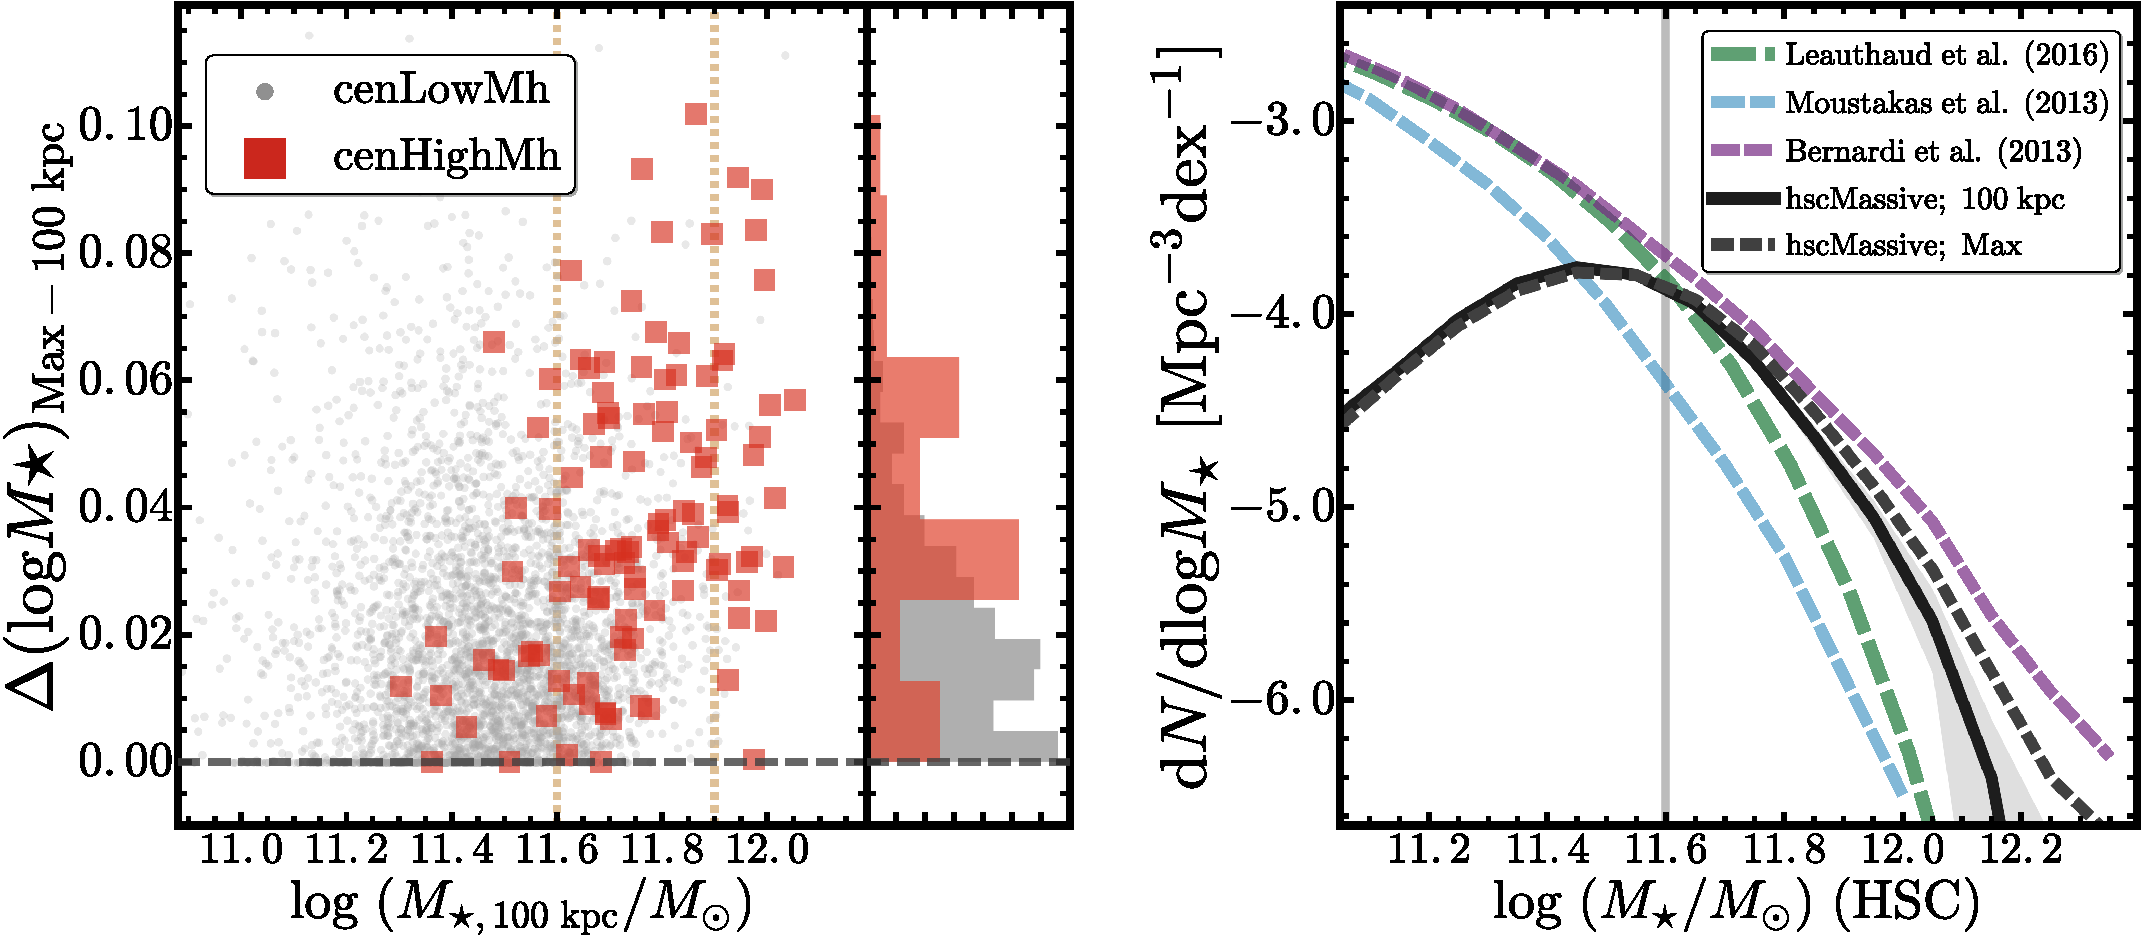
\includegraphics[width=\textwidth]{fig/redbcg_discussion_5}
      \caption{
      \update{
          \textbf{Left}: Relation between \mtot{} and the logarithmic mass difference 
          between \mmax{} and \mtot{} for both \rbcg{} (red square) and \nbcg{} 
          (grey dot) galaxies.  The format is very similar to the left figure of 
          Fig.\ref{fig:smf1}.~~
          \textbf{Right}: The stellar mass volume-density distributions of massive galaxies 
          after combining the \rbcg{} and \nbcg{} samples together, using both 
          \mtot{} (black solid line) and \mmax{} (black dash line). 
          The uncertainty for distribution using \mtot{} is shown in grey shaded region.  
          Here, we also compare the distributions with SMF from previous works: 
          (a): SDSS galaxies at $z\sim 0.1$ from \citet{Bernardi2013}; the \mstar{} is 
          based on photometry from 2-D \ser{}$+$Exponential model fitting; 
          (b): SDSS galaxies at $z\sim 0.1$ from \citet{Moustakas13} based on 
          improved SDSS \texttt{cModel} photometry; 
          (c): \texttt{S82-MGC} galaxies at $0.15 < z< 0.43$ from 
          \citet{Leauthaud2016} based on PSF-matched SDSS-UKIDSS photometry.
          Please see text for more details of the comparison.
          }}
      \label{fig:discussion_1}
  \end{figure*}
%% ------------------------------------------------------------------------------------ %%

%% ------------------------------------------------------------------------------------ %% 
  \begin{figure}[bt!]
      \centering 
      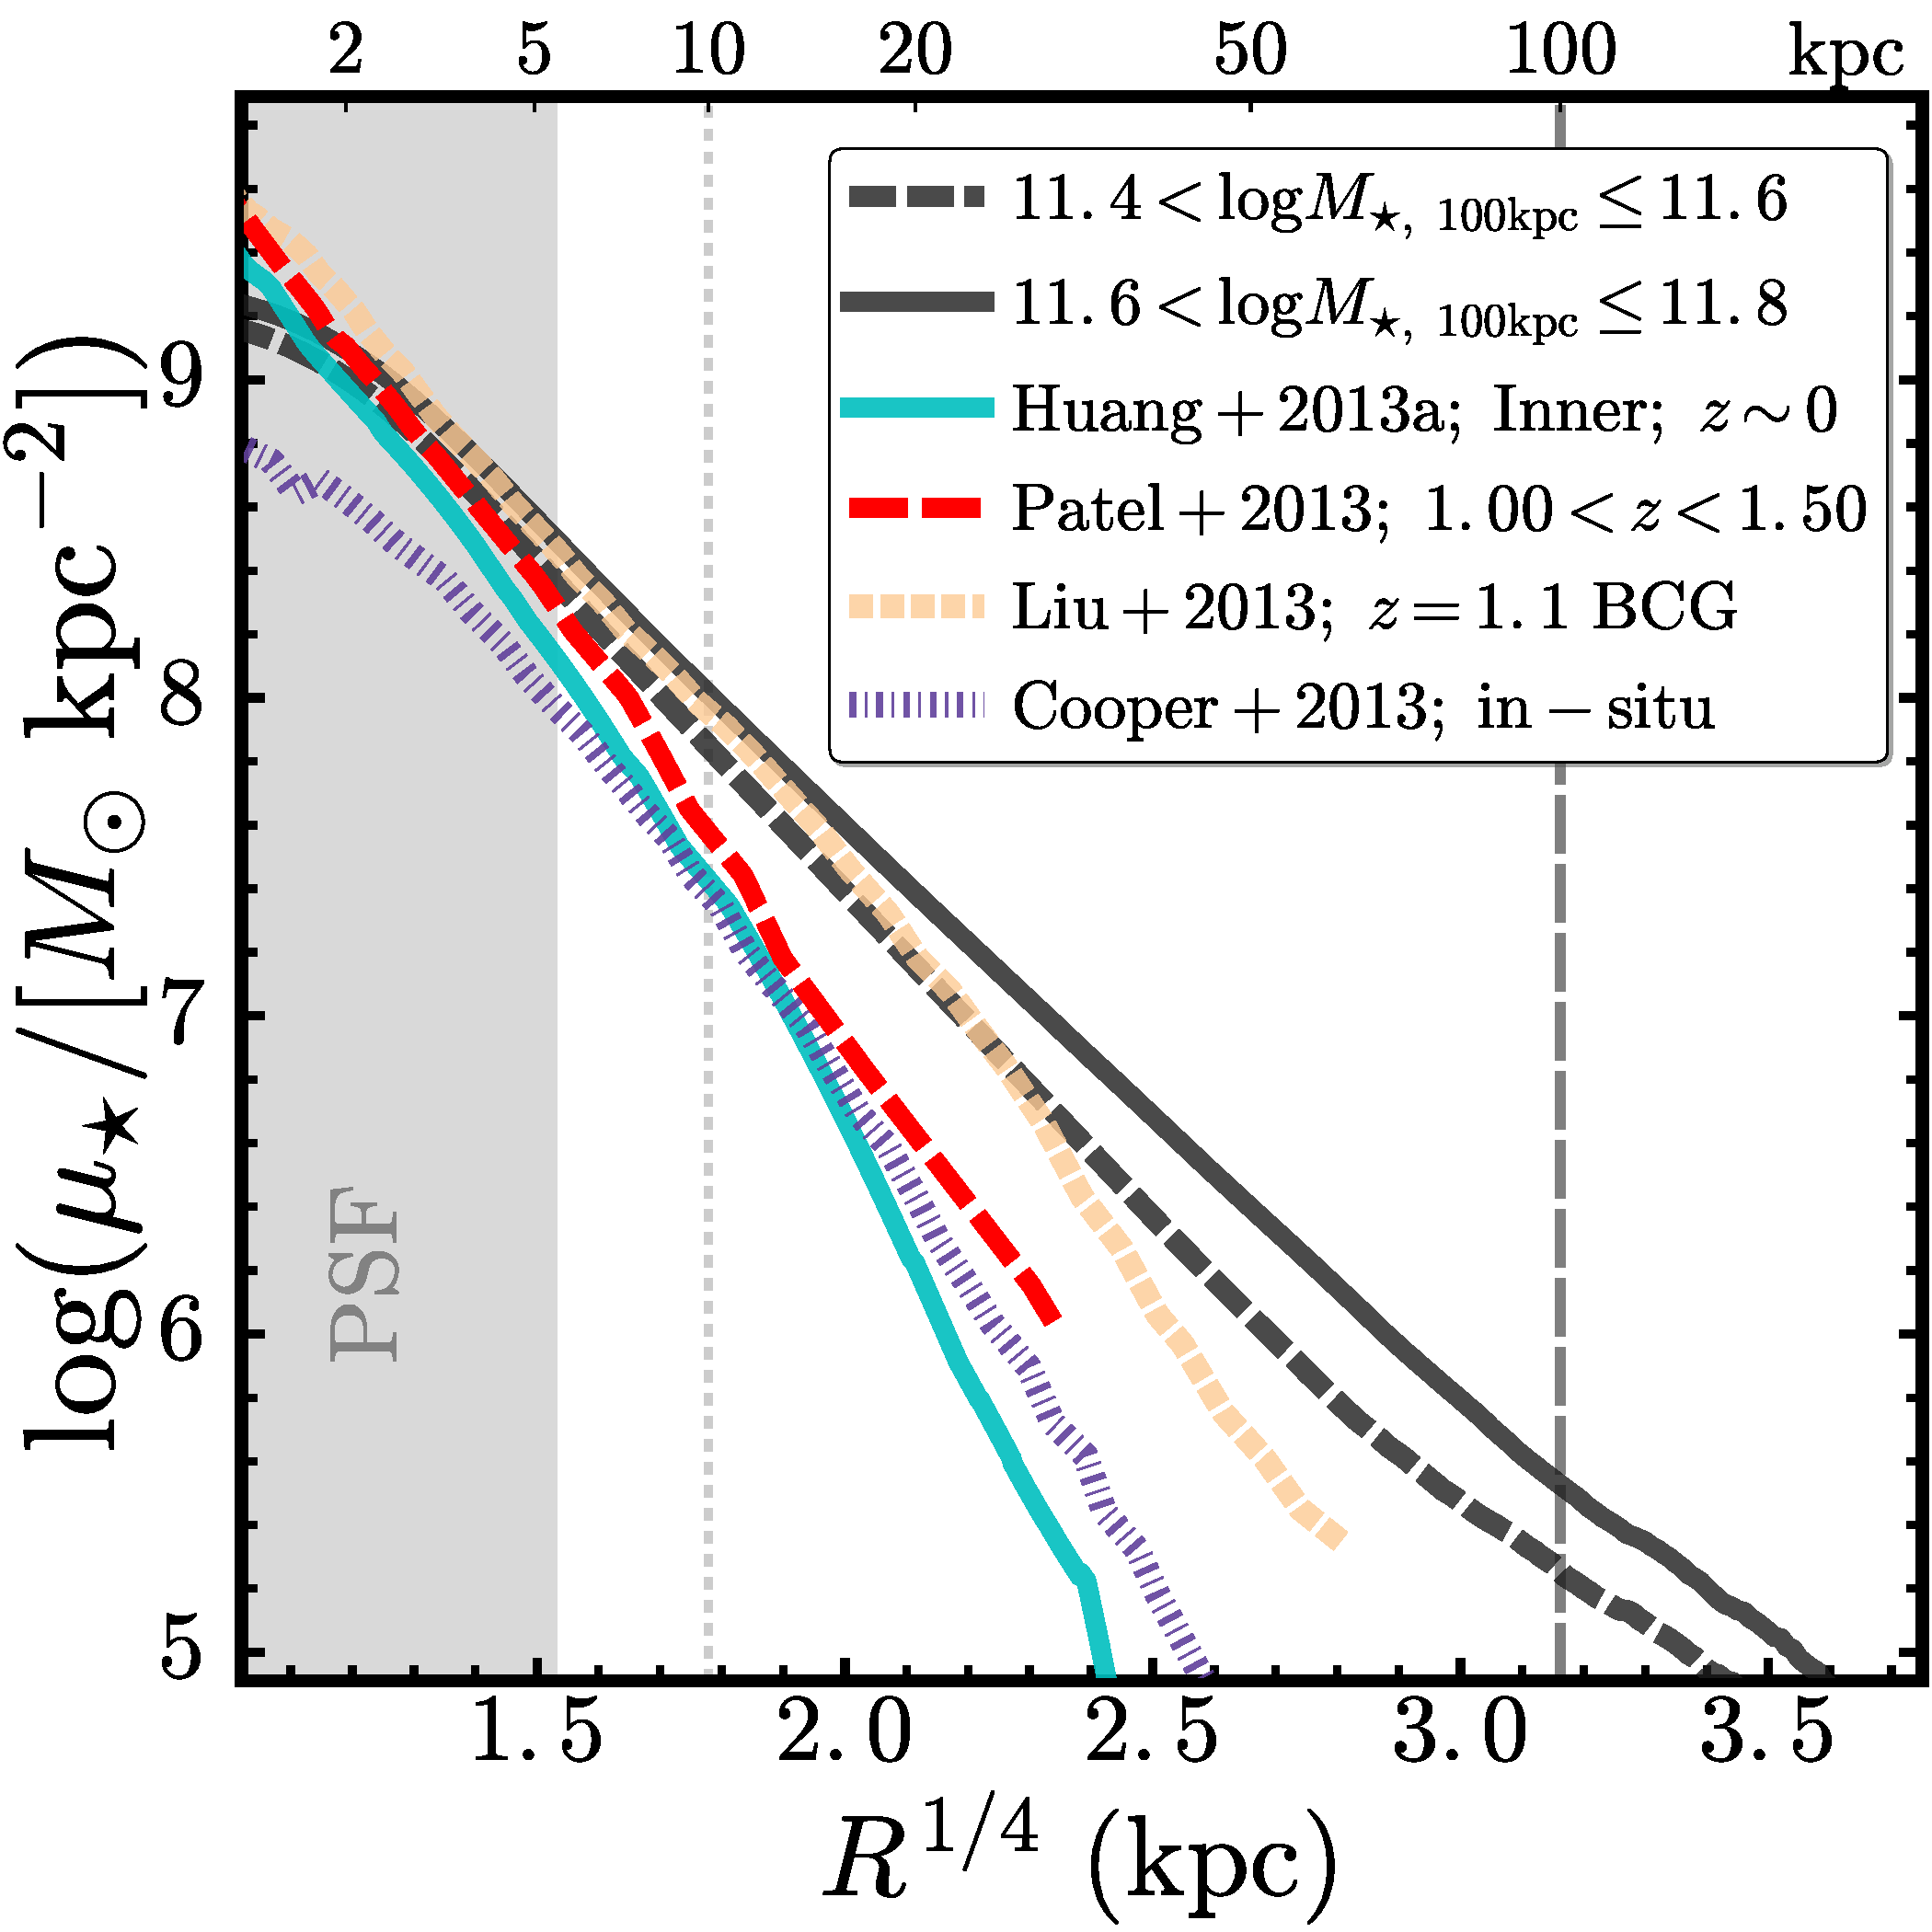
\includegraphics[width=\columnwidth]{fig/redbcg_discussion_1}
      \caption{Comparison of the average \mden{} profiles of massive galaxies in the 
          two lower \mtot{} bins from Fig.\ref{fig:avg_prof} with other observations 
          and simulations, focusing on the inner region. 
          The format is similar with the right panel of Fig.\ref{fig:avg_prof}.
          We include: 
          1) the average \mden{} profile of inner component from structure 
          decomposition of massive elliptical galaxies at $z\sim 0$ from 
          \citet[][Cyan, solid]{Huang2013a}; 
          2) the average \mden{} profile of massive galaxies at $1.0 < z < 1.5$ 
          from \textit{HST} observations in \citet[][Red, dashed]{Patel2013}; 
          3) the average \mden{} profile of the ``in-situ'' stellar components in 
          simulated massive halos from \citet[][Purple, dot-dashed]{Cooper13};
          4) the \mden{} profile of the very massive cD galaxy at $z\sim 1.1$ 
          discovered by \citet[][Yellow, dashed]{Liu2013} in the Hubble 
          Ultra-Deep Field.}
      \label{fig:discussion_2}
  \end{figure}
%% ------------------------------------------------------------------------------------ %% 

\section{Discussions}
    \label{sec:discussion}
    
    In the past decade, the mass assembly and structural evolution of massive ETGs 
    remains as an active topic.  
    More and more convincing observations of massive galaxies at high redshift reveal that
    the progenitors of massive elliptical galaxies are quite different in structure
    comparing with their local decedents (e.g. \addref{}).  
    Collectively, they need to increase their ``size'' ($R_{\mathrm{e}}$) by a factor of 
    2 to 4 (e.g. \addref{}) without changing their inner \mden profile (e.g. \addref{})
    and central stellar velocity dispersion (e.g. \addref{}) much in the last 8-10 Gyrs.  
    Owing mainly to better numerical simulations, the challenge of ``size''-evolution 
    seems to be eased by the promising ``two-phase'' scenario under the framework of 
    hierarchical formation of galaxy (e.g.\addref{}). 
    Under this picture, the inner region of massive galaxies mostly consist of stars 
    formed within the halo of the main progenitor through intense dissipative processes 
    at high redshift.  
    Later, after the active star formation is quenched in these massive systems, their 
    mass assembly history becomes dominated by accretions of satellites.  
    Based on the prediction of merger tree and current understanding of satellite 
    population around massive galaxies, most these merging events are likely to be 
    minor ones, and without involving much gas dissipation.  
    Since such minor, dry merger basically redistributes stars onto the outer envelope 
    of the central galaxy, it becomes the most promising solution to the ``size-evolution''
    puzzle.  
    However, it raises additional questions at the same time. 
    The most pressing one would be the expected ``environmental''-dependence of structures 
    of massive central galaxies. 
    As minor merger is expected to be more frequent in denser environment, the mass assembly 
    history and \mstar{} distribution of central galaxies should show dependence on \mhalo{}
    or even other properties of the host halo.  
    For instance, centrals in more and less massive halos could have different 
    slopes and/or scatters in their mass-size relation (e.g. \addref{}).  
    Yet, no clear evidence of such dependence has been found. 
    In this work, taking advantage of the deep photometry from the HSC survey and looking 
    into the detailed \mden{} profiles, we clearly see evidence that the \textbf{structure
    of massive central galaxies, both the inner and outer parts, does show dependence on 
    the halo mass}. 
    Here, we briefly discuss the physical causes of this dependence, potential caveats, 
    and more scientific implications.  
    
    Firstly, the comparisons of the \mden{} profiles suggest that \textbf{\mhalo{} does 
    not play a central role in shaping the structure of massive central galaxies}.  
    It appears that massive central galaxies at \logms{}$\geq 11.5$ were shaped by 
    same physical processes in more and less massive halos.  
    At both fixed \mtot{} and \minn{}, centrals from cluster-level halos do not form a 
    unique population. 
    Instead, their individual \mden{} profiles greatly overlap with the ones in halos of 
    small group. 
    At similar \mtot{}, even their median \mden{} profiles only show quite subtle 
    differences. 
    For the \rbcg{} sample, this is similar to the results of \citep{Zhao2015} that 
    a considerable fraction of nearby BCGs (34\%) does not fall into the ``cD'' class.
    From the smooth distributions of \mden{} profiles on Fig.\ref{fig:prof_1} 
    and Fig.\ref{fig:prof_4}, it is even harder to draw a clear difference 
    between ``cD'' galaxy and ``normal elliptical''. 
 
    At the same time, \textbf{the \mhalo{}-dependence we found do fit the expectations 
    of the ``two-phase'' scenario at first glance}. 
    For central galaxies with similar stellar mass at the end of the first phase, 
    their subsequent, accretion-dominated mass assembly naturally relates to \mhalo{}, 
    which determines the number and mass distributions of satellites. 
    Therefore, centrals of more massive halos should accumulate more extended stellar 
    envelope during the second phase, exactly as we find in the \mden{} profile 
    comparison of the \minn{}-matched samples (see Fig.\ref{fig:prof_4}).
    Under the ``two-phase'' formation scenario, the stellar content of massive galaxies
    can be broadly separated into the ``in-situ'' and ``accreted'' components. 
    At fixed \mtot{}, the differences of median \mden{} profiles could reflect 
    different relative fraction of these two components. 
    Recent simulations indicate that (1) the fraction of accreted stars could have 
    a steep correlation with total stellar mass; (2) for \logms$\geq 11.5$ galaxies,
    the accreted component starts to dominate within the $R_{\mathrm{e}}$.  
    Given that (1) the ``transition radius'' between the two median profiles is around
    15-20 kpc (see Fig.\ref{fig:prof_1}); and (2) the differences become more 
    significant at higher mass end, it is likely the \mhalo{}-dependence of structure
    at fixed total stellar mass is driven by the higher fraction of accreted stars 
    in more massive halos.  
    To confirm this inference, in Fig.\ref{fig:discussion_1}, we compare the median 
    \mden{} profiles of the \mtot{}-matched \rbcg{} and \nbcg{} samples at 
    $11.5\leq$\logms{}$<11.7$ with the median profiles of 
    (1) massive ETGs at $1.0 < z < 1.5$ that are considered the progenitors of 
    $\sim 10^{11.5} M_{\odot}$ ETGs at $z=0$ (\citealt{Patel2013}).  
    After this redshift range, their mass growth should be dominated by mergers.  
    (2) inner components of $z=0$ $10^{11.4} M_{\odot}$ ellipticals from 2-D decomposition
    (\citealt{Huang2013a}). 
    \citep{Huang2013b} showed that these structures are quite similar to the compact 
    progenitors at higher redshift in many aspects.  
    (3) the ``in-situ'' components of simulated galaxies in massive halo of 
    \citep{Cooper13} using particle-tagging technique (the inner few kpc is quite 
    uncertain due to the resolution).  
    Regardless the small difference in median \mstar{} and details in \m2l{} estimates, 
    the comparison first confirms that \minn{} is indeed not a bad proxy of the in-situ 
    mass; meanwhile, it also highlights that structural difference between \rbcg{} and 
    \nbcg{} are driven by region that is not dominated by ``in-situ'' stars. 
    Since most of these samples in comparison are not as extreme as the massive 
    \rbcg{} galaxies, we also compare with a uniquely massive BCG at high redshift: 
    a $10^{11.4} M_{\odot}$ BCGs with distinctive envelope at $z\sim 1.1$ 
    (\citealt{Liu2013}).  
    It is interesting to see that its \mden{} profile follows the median profile of 
    \rbcg{} nicely until 20 kpc; then it becomes much steeper in the outskirt.  
    This is quite consistent with the expectation that the inner part of the BCGs 
    should be well developed at $z\sim 1$, but the extended stellar envelope is still 
    assembling.  
    
    Also, it is worth noting that the relative flatten inner \mden{} profile of \rbcg{}
    at fixed \mtot{} could be an interesting feature, although we currently lack of the 
    resolution to investigate region $\leq 3$ kpc.  
    It is known that major-merger induced coalesce of super-massive black hoes (SMBHs)
    can create flattened inner profile (e.g. \citealt{Milosavljevi2002}), and recent 
    discoveries of massive BCGs with very large core 
    (a few kpc; e.g. \citealt{Postman2012, LopezCruz2014}) further complicate the picture.
    On Fig.\ref{fig:m100_m10_A}, there are a few \rbcg{} galaxies with quite low 
    \minn{} at high \mtot{} end. 
    After examining their images, we conclude the low \minn{} is not caused by problematic
    photometry or exceptionally bad seeing; they could also be massive BCGs with very 
    flattened inner \mden{} profiles.  
    Besides the SMBH-merger theory, strong adiabatic expansion induced by strong AGN 
    feedback was proposed to modify the inner mass distribution (e.g. \citealt{Fan2008}). 
    The potential impact of these processes to massive galaxies, and their dependence on 
    halo mass would be an interesting topic to investigate in the future.  
    
    \song{Move a big paragraph to Results} 
    
    \song{Ok, I'll see how to make it happen; this sounds abrupt since I used 
    to have several subsections in the discussion section.}
    \alexie{The beginning part of this paragraph sounds to me like the summary section. You could move part of this to summary and put it in bullet piont format.}. In the end, we want to emphasis once more \textbf{the importance of deep image 
    and appropriate method of photometry in studying the structure and assembly 
    history of galaxies}. 
    With the help of deep HSC images, we reliably reveal the extended stellar 
    structures around large sample of massive central galaxies out to more than 
    100 kpc.  
    And, using model-independent method, we found that 
    (1) previous de~Vaucouleur or single-\ser{} modeling method on shallower SDSS
    images underestimates the total mass of massive galaxies; 
    (2) even using deep HSC images, photometric method like \cmodel{} also tends 
    to underestimate the mass. 
    For these massive central galaxies, their extended mass distributions are 
    simply beyond the capability of the simply modeling method.  
    In addition, since the slope and mass contribution of the outer envelope 
    depend on not only the total stellar mass, but also likely the halo mass. 
    Applying the same oversimplified model to galaxies across a large range of 
    mass and environment could result in both underestimated and biased mass 
    estimates that can stop us getting accurate stellar mass function at the 
    high-mass end and studying potential environmental dependence of structures. 
    Moreover, these results also raise crucial questions like: 
    \textbf{What is the definition of ``total'' stellar mass of galaxy? 
    And, what is the most informative definition of stellar mass in the studies 
    of galaxy evolution?}.  \alexie{I think we can expand the discussion around this topic. We'd like to say somehting about the impact of total luminosity on the SMF. How about moving the left hand of Figure 3 here? What is the current volume of your data set compared to the volume of SDSS? I think we should emphasize the impact of stellar mass estimate on the SMF, especialy the large impact it has for BCGs}.
    \song{As mentioned earlier, I can expand the discussion easily with the help 
    from another figure, comparing with SMF from other people's work?//}
    
    \alexie{Yes, the only thing that I just realized and pointed out in the ealier SMF figure is that to compare the SMF, we need to include everything, not just centrals. There are two options: 1) just show the impact on the SMF for centrals (the figure you have already) or 2) include all the galaxies and compared with previous work. I think that 2) is a paper inself and is beyond the scope of the papers (it becomes "Mission Creep").}
    
    
    \alexie{I thought of another interesting aspect to add to the discussion. This I think is perhaps a nice angle to discuss. The total luminosity of a galaxy has an impact on abundance matching. Do you have the "luminosity" that you would get for each galaxy if you assumed a single sersic fit for example? If so, we could do the following. Assume a one-to-one mapping between halo mass and your M100. Then plot Mhalo versus the stellar mass inferred from either cmodel of the single sersic fit. Then we can quote the scatter in $\log(M_*)$ at fixed Mhalo that this introduces. This figure will be very relevent for the Santa Barabara workshop!}
    \song{We do not have results from single Sersic models; at least not reliable enough 
    to be used here, mostly because single Sersic works terribly for these galaxies.
    We do have \mcmodel{}, but sorry that I failed to follows the logic here, basically this is 
    the difference between \mtot{} and \mcmodel{} expressed in a different way, and I am not 
    sure the scatter is due to the scatter of the mhalo-mstar relation, as the cModel 
    ones are underestimated due to technical reasons; We can bin the \rbcg{} galaxies 
    into a narrow $\lambda$ bin thoug, e.g. $30< \lambda < 40$, and see the scatter of 
    \mcmodel{}, \minn{}, and \mtot{}. We can certaintly shows that the scatter is larger 
    for mass using larger radius.  I think this point is important for the discussion
    of the intrinsic scatter of the mhalo-mstar relation, and at very similar mhalo,
    the outer structure may trace other properties of the halo. Let me know what do 
    you think.\\}
    
    \alexie{THe same idea holds if we use our M100 mass and cmodel. The points is just to evaluate how much extra scatter you introduce because of many people simple use naive luninosities when they do abundance mathcing. Your previous figures show that the luminosities of massive galaxies may be severaly underestiamted. How much impact does this have on abundance mathcing? How much extra scatter does it introduce?}
    
    \alexie{Finally, another quick discussion paragraph could be related to finding BCGs. It would be interesting to have a plot of the magnitude gap between Pcen1 and Pcen 2 (the most likely and the second most likely central) with cmodel versus your estimates. It would be nice to show that having a better luminosty estimate will enable you to identify the BCG better (is this true?)}.
    \song{This is interesting, and I don't know if it is true. It requires more works as 
    I do not have the profiles for all PCEN2 galaxies, I only do it when they are more 
    massive than the threshold.  Can we save this for later, I mean, after we send around 
    the draft.  Although I do compare the structures of really massive satellites in 
    these clusters with the \nbcg{} galaxies, and the results show little difference,    basically shows that the structure difference could be unique for central galaxies. 
    I originally show a figure for this, and will send you along the e-mail.}
    
    \alexie{If it is too much, work, skip this idea! We dont want mission creep.}
    
    In this work, we choose mass enclosed by different, but fixed physical 
    apertures, and find promising scientific applications for massive galaxies. 
    But, we recognize that they may not be the best choice. 
    For instance, central galaxies of massive halos like BCGs are known to be
    surrounded by diffuse stellar component that does not follow the potential 
    of the central galaxy (the intra-cluster light, or ICL; e.g. \addref{}).
    In theory, it can contribute a large amount of stellar mass out to very 
    large radius (e.g. \addref{}).  
    Using the definition of \mtot{}, we can not separate the potential 
    contribution of ICL in our \rbcg{} galaxies; and this could make complicate
    the discussion of environmental dependence.  \alexie{I am not sure I agree here. What is the "ICL"? How can is physically be defined? Can one robustly distinguish an "ICL" component from the galaxy component and how? Is the ICL similar to the "cD" enveloppe in the sense that we use these words all the time, but in practice, these are just one extrema of a continous galaxy population?}
    Since most of the \rbcg{} galaxies in our sample belong to low-mass cluster 
    like the Virgo or Fornax, we do not expect the ICL component can makes a 
    smooth and significant contribution to the \mden{} profiles (e.g. \addref{}).
    Even removing all \rbcg{} galaxies in $\lambda > 40$ clusters will not change 
    our findings.  
    However, it is still important to ask whether should we include the ICL when 
    estimating the mass of central galaxies in massive halos.  \alexie{But what is the ICL?}
    \song{The observational definiiton is very vague; and the theoretical one is 
    very hard to achieve through observation, basically the stars that follows the 
    potential of the clsuter.} \alexie{Exactly. Which is why I think we dont want to go into a big discussion on this.}
    And, if the answer is no, which is the best way to separate the ICL component? 
    In literature, most works studied ICL by subtracting the model for inner part
    of the central galaxy (e.g. \addref{}).  
    As we show in this work, when extended stellar envelopes are revealed around 
    massive galaxies in large range of stellar and halo mass, we may have to 
    reconsider this approach \alexie{I agree with this phrase, this is good to point out.}.
    \song{I think I understand your point here. The thing with ICL is that any 
    conclusion so far is quite uncertain, so I can reorganize this paragraph, 
    point out the interesting question first, discuss it a little bit, but also 
    shows a caveat that say ICL could play a role here, and if it does, how could 
    they change our results.}
    
    \alexie{I'm saying more than that. I'm saying that I don't beleive that there is necessarly a firm distinction between the galaxy and the "ICL". Might be easier to chat about this on Skype.}
 
%    As suggested by the popular two-phase formation scenario of massive galaxies, 
%    the inner 5-10 kpc of these galaxies (within 0.5-1$xR_{\mathrm{e}}$) is 
%    dominated by stars formed in intensive dissipative processes at high redshift, 
%    and is less affected by the succeeding merging events.  
%    This picture is broadly supported by the redshift evolution of \mden{} profile
%    of massive galaxies (\addref), structure decomposition of nearby massive galaxies 
%    (\addref), and their radial distributions of stellar population (\addref).      
%    Certainly, major merger can induce violent relaxation process that modifies the 
%    stellar mass distribution even in the central region, and must happen to 
%    these massive galaxies in last 6-8 Gyrs, it may not invalidate the above assumption.
%    For galaxy this massive, the last major merger event is highly likely to be
%    non-dissipative, and the redistribution of stars is basically according to their 
%    binding energy in the host halo.  
%    The inner region of the final merger remnant is still mostly composed 
%    of the ``in-situ'' stars from the two progenitors.  
 

   
%\subsection{Impact from ``Fossil Galaxies''}
%
%    ``Fossil galaxy'' is the most massive galaxy in a ``fossil group/cluster''
%    system.
%    According to the commonly adopted definition, ``fossil'' systems are the 
%    group or cluster with high X-ray luminosity and large magnitude gap between 
%    the two brightest galaxies (\addref: Ponman1994; Jones2003). 
%    Both observations and simulations suggest that they could represent the 
%    final stage of the hierarchical merging process in a group/cluster mass
%    halo that is formed at very early epoch (e.g.\ \addref: 
%    Khosroshahi2004, 2007; DOnghia2005; Dariush2007).
%    Under this interpretation, at fixed halo mass, the central galaxy of 
%    a fossil system typically has larger stellar mass than the one in normal 
%    system (e.g.\ Harrison2012), as it has ``consumed'' most satellites 
%    early on; 
%    However, the ``low richness'' of a fossil system makes it difficult for 
%    red-sequence finder like \redm{}~to reliably identify 
%    (e.g.\ Figure~17 of Sadibekova2014).  
%    If some massive ETGs in our \nbcg{} sample are actual the centrals 
%    galaxies of fossil clusters, it could bias our conclusions about the 
%    relation between structure and ``environment''.  
%    
%    Although it is possible that fossil systems formed earlier than normal 
%    clusters, the difference in detailed merging history is still unclear, 
%    hence it is hard to imagine the structural differences between fossil 
%    central galaxies and regular BCGs with same \mstar{}.  
%    Naively speaking, more frequent mergers for fossil centrals should result 
%    in more extended stellar envelope.  
%    However, the distributions of epoch and mass-ratio of those mergers also 
%    matter. 
%    
%    The lack of any difference in stellar population properties may suggest 
%    It is still not clear how the mass assembly history of fossil central 

%% ------------------------------------------------------------------------------------ %% 

\section{Summary and Future Plans}
    \label{sec:summary}

    \update{ 
    In this work, we study the how environment (halo mass) affects the structures and
    assembly history of massive central galaxies using deep images from the Subaru HSC 
    survey.
    With the help of these high-quality data, we map the stellar mass distributions of 
    large numbers of massive central galaxies at $0.3 < z < 0.5$ out to $>100$ kpc, 
    and discussing their environmental dependence after grouping them into centrals of 
    halos more and less massive than \mhalo{}$\sim 10^{14} M_{\odot}$. 
    The main results here are:}
    
    \begin{enumerate}
        \item \update{
            We find that the ``total'' \mstar{} of these massive galaxies could be 
            significantly underestimated when shallow image (e.g. the SDSS ones) 
            and/or imperfect model assumption (e.g. the \texttt{cModel}) are used.
            In different with previous works, this result does not depend on stacking 
            analysis or any parametric model. 
            Moreover, the level of such underestimation could also depend on the 
            stellar mass. 
            This should be carefully taken into account when discussing important 
            topics like the stellar mass function and its evolution.
            }
        \item \update{
            At fixed \mstar{} within 100 kpc, we find that the massive central 
            galaxies in more and less massive halos have subtle, but systematic 
            differences in their \mden{} profiles when their ellipticity and optical 
            color profiles are very similar. 
            On average, the ones from denser environments have slightly shallower 
            inner \mden{} profiles while showing more prominent outer envelope.
            }
        \item \update{
            Meanwhile, when matched at the same \mstar{} within inner 10 kpc--a 
            proxy of the \mstar{} formed in the the ``in-situ'' channel, we find 
            that the ones in more massive halos possess much more extended stellar 
            envelope in the outskirts than the ones in smaller halos when the 
            \mden{}, ellipticity, and optical color profiles inside 10 kpc show 
            no dependence on environment. 
            }
        \item \update{
            The \mstar{}-size relation also reflects the subtle environmental 
            dependence as the central galaxies from more massive halos have 
            slightly higher $R_{\mathrm{50}}$ at fixed \mtot{}. 
            We further suggest that the relation between \mtot{} and 
            \minn{}\footnote{or any better proxy of total \mstar{} and the mass 
            formed in the ``in-situ'' phase.} can be useful tool in diagnosing the
            assembly history of these massive galaxies and its relation to their 
            dark matter halos. 
            }
    \end{enumerate}

	%\subsection{Future Improvements}
    %\label{ssec:future}
    These results are broadly consistent with the prediction of the ``two-phase''
    scenario: the massive central galaxies in more massive halos should experience 
    more minor, dry mergers that accumulate more stars in the outskirts. 
    These results also highlight the advantages of HSC survey in studying the 
    evolution of massive galaxies.
    Upon finishing this work, the HSC survey has already doubled its sky 
    coverage to $\sim 200$ deg$^2$, and provides a much larger sample of massive 
    central galaxies. 
    At the same time, we will work on better data reduction of HSC images by 
    improving the deblending in crowded regions and the accuracy of background 
    subtraction. 
    This can help provide more reliable SED fitting results, and push the 
    photometric limit to even lower surface brightness.  
    
    Right now, we still rely on the \redm{} catalog from SDSS and spectroscopic 
    redshift from SDSS and BOSS.  
    Running \redm{} algorithm or similar group/cluster finder on HSC catalogs 
    can greatly help us extend the discussion to lower \mhalo{} and higher 
    redshift. 
    Better selection of satellites in massive halos will also open up the 
    possibility to study ``environment'' within the halo.
    It is interesting to see whether there is any structural difference
    between central and satellite galaxy at similar \mstar{}.
    
    We will work on careful 2-D photometric modeling to these massive galaxies.
    Under the same principle outlined by \citealt{Huang2013a}, we will explore 
    different models, and gradually build up the complexity to fit these galaxies 
    better.
    With the 2-D modeling approach, we can deal with the seeing and background
    subtraction easier, and provide better maps the stellar mass distributions. 
    We are also working on characterizing the color distributions of these 
    galaxies better via multi-band modeling with reasonable constraints (e.g. 
    \citealt{Huang2016}). 
    
    Primarily designed as a cosmological endeavor, the HSC survey has excellent 
    images to greatly improve the the weak lensing analysis of massive galaxies. 
    The next major step will be to investigate the connections between massive 
    galaxies and their halos with the help of the weak lensing signals for 
    different groups of massive galaxies (e.g. binned by \mtot{}, \minn{}, 
    size\etal).
    Joining the stellar mass distributions and the weak lensing signals together, 
    we can trace the impacts from a series of physical processes 
    (strength and type of AGN feedback, merger rate, typical mass ratio of mergers
    \etal). 
    To help us have better physical insights, we will directly compare our results 
    with predictions from cosmological hydro-simulations such as 
    Illustris (\citealt{Vogelsberger2014}, \citealt{Genel2014}), 
    EAGLE (\citealt{Schaye2015}, \citealt{Crain2015}), 
    or \textit{Horizon-AGN} (\citealt{Dubois2014}). 

%% ------------------------------------------------------------------------------------ %% 
  
  
\acknowledgements

  % HSC part
  The Hyper Suprime-Cam (HSC) collaboration includes the astronomical communities of 
  Japan and Taiwan, and Princeton University.  The HSC instrumentation and software were
  developed by the National Astronomical Observatory of Japan (NAOJ), the Kavli Institute
  for the Physics and Mathematics of the Universe (Kavli IPMU), the University of Tokyo,
  the High Energy Accelerator Research Organization (KEK), the Academia Sinica Institute
  for Astronomy and Astrophysics in Taiwan (ASIAA), and Princeton University.  
  Funding was contributed by the FIRST program from Japanese Cabinet Office, the Ministry 
  of Education, Culture, Sports, Science and Technology (MEXT), the Japan Society for 
  the Promotion of Science (JSPS), Japan Science and Technology Agency (JST), the
  Toray Science Foundation, NAOJ, Kavli IPMU, KEK, ASIAA, and Princeton University.
   
  % SDSS part
  Funding for SDSS-III has been provided by the Alfred P. Sloan Foundation, the
  Participating Institutions, the National Science Foundation, and the U.S.  Department of
  Energy. The SDSS-III web site is http://www.sdss3.org.  SDSS-III is managed by the
  Astrophysical Research Consortium for the Participating Institutions of the SDSS-III
  Collaboration including the University of Arizona, the Brazilian Participation Group,
  Brookhaven National Laboratory, University of Cambridge, University of Florida, the
  French Participation Group, the German Participation Group, the Instituto de Astrofisica
  de Canarias, the Michigan State/Notre Dame/JINA Participation Group, Johns Hopkins
  University, Lawrence Berkeley National Laboratory, Max Planck Institute for
  Astrophysics, New Mexico State University, New York University, Ohio State University,
  Pennsylvania State University, University of Portsmouth, Princeton University, the
  Spanish Participation Group, University of Tokyo, University of Utah, Vanderbilt
  University, University of Virginia, University of Washington, and Yale University.
  
  % Pan-STARRS1 part
  The Pan-STARRS1 Surveys (PS1) have been made possible through contributions of the 
  Institute for Astronomy, the University of Hawaii, the Pan-STARRS Project Office, 
  the Max-Planck Society and its participating institutes, the Max Planck Institute 
  for Astronomy, Heidelberg and the Max Planck Institute for Extraterrestrial Physics, 
  Garching, The Johns Hopkins University, Durham University, the University of Edinburgh, 
  Queen's University Belfast, the Harvard-Smithsonian Center for Astrophysics, the Las 
  Cumbres Observatory Global Telescope Network Incorporated, the National Central 
  University of Taiwan, the Space Telescope Science Institute, the National Aeronautics 
  and Space Administration under Grant No. NNX08AR22G issued through the Planetary 
  Science Division of the NASA Science Mission Directorate, the National Science 
  Foundation under Grant No. AST-1238877, the University of Maryland, and Eotvos 
  Lorand University (ELTE).
  
  % LSST software
  This paper makes use of software developed for the Large Synoptic Survey 
  Telescope. We thank the LSST Project for making their code available as free 
  software at http://dm.lsstcorp.org.
 
  % Software
  This research made use of:
  \href{http://www.stsci.edu/institute/software_hardware/pyraf/stsci\_python}{\texttt{STSCI\_PYTHON}},
      a general astronomical data analysis infrastructure in Python. 
      \texttt{STSCI\_PYTHON} is a product of the Space Telescope Science Institute, 
      which is operated by AURA for NASA;
  \href{http://www.scipy.org/}{\texttt{SciPy}},
      an open source scientific tools for Python (\citealt{SciPy});
  \href{http://www.numpy.org/}{\texttt{NumPy}}, 
      a fundamental package for scientific computing with Python (\citealt{NumPy});
  \href{http://matplotlib.org/}{\texttt{Matplotlib}}, 
      a 2-D plotting library for Python (\citealt{Matplotlib});
  \href{http://www.astropy.org/}{\texttt{Astropy}}, a community-developed 
      core Python package for Astronomy (\citealt{AstroPy}); 
  \href{http://scikit-learn.org/stable/index.html}{\texttt{scikit-learn}},
      a machine-learning library in Python (\citealt{scikit-learn}); 
  \href{http://www.astroml.org/}{\texttt{astroML}}, 
      a machine learning library for astrophysics (\citealt{astroML});
  \href{https://ipython.org}{\texttt{IPython}}, 
      an interactive computing system for Python (\citealt{IPython});
  \href{https://github.com/kbarbary/sep}{\texttt{sep}} 
      Source Extraction and Photometry in Python (\citealt{PythonSEP});
  \href{https://jiffyclub.github.io/palettable/}{\texttt{palettable}},
      color palettes for Python;
  \href{http://dan.iel.fm/emcee/current/}{\texttt{emcee}}, 
      Seriously Kick-Ass MCMC in Python;
  \href{http://bdiemer.bitbucket.org/}{\texttt{Colossus}}, 
      COsmology, haLO and large-Scale StrUcture toolS (\citealt{Colossus}).

%%%%%%%%%%: Bibliographic Section %%%%%%%%%%

\bibliography{redbcg}

%%%%%%%%%%: Appendix Section %%%%%%%%%%%%

\appendix

%% ------------------------------------------------------------------------------------ %% 

\section{A. Basic Statistical Properties of the Sample} 
	\label{app:basic}
    
    \update{
    In the top-left figure of Fig.\ref{fig:sample_stats}, we show the \mtot{}-color 
    relations using the $k$-corrected $g-r$ color for the \rbcg{} and \nbcg{} 
    samples. 
    Both samples follow the same tight ``red-sequence'' with very little contamination 
    from star-forming galaxy in the ``blue cloud''.
    And, at fixed \mtot{}, we see little offset in color distributions of the two 
    samples suggesting that both samples consist of old quiescent galaxies with 
    similar average stellar population properties.  
    This is consistent with previous result that suggests the average stellar 
    population of massive central galaxy does not depend on \mhalo{} 
    (e.g.\ \citealt{Park2007}).  
    To look into the potential environmental dependence of structure, we will 
    focus on the mass range of $11.6 \le$\logmtot{}$\le 11.9$, where both samples 
    have acceptable completeness, and their \mtot{} distributions greatly overlap
    (see the normalized distributions of \mtot{} in the bottom-left panel of 
    Fig.\ref{fig:sample_stats}). 
    The similar situation applies to the \minn{} distributions as well, where 
    the two samples overlap the most within $11.2 \le$\logmtot{}$\le 11.6$, but 
    have quite different relative distributions.}
    
    \update{
    Due to the different sources of redshift for the \rbcg{} and \nbcg{} samples, 
    the two samples have somewhat different redshift distributions 
    (right figure of Fig.\ref{fig:sample_stats}), even within the 
    $11.6 \le$\logmtot{}$\le 11.9$ mass bin.  
    Apparently, the redshift distribution of the \nbcg{} sample skews toward 
    higher-$z$ end, primarily due to the contribution of BOSS spec-$z$.
    This could bias the comparison of \mden{} profiles and other properties 
    (please see Appendix\ref{app:D} for more details).  
    We will address this via matching the two samples in both mass and redshift
    distributions carefully before any comparison (see Appendix~\ref{app:match}).}
    
%% ------------------------------------------------------------------------------------ %% 
  \begin{figure*}[t!]
      \centering 
      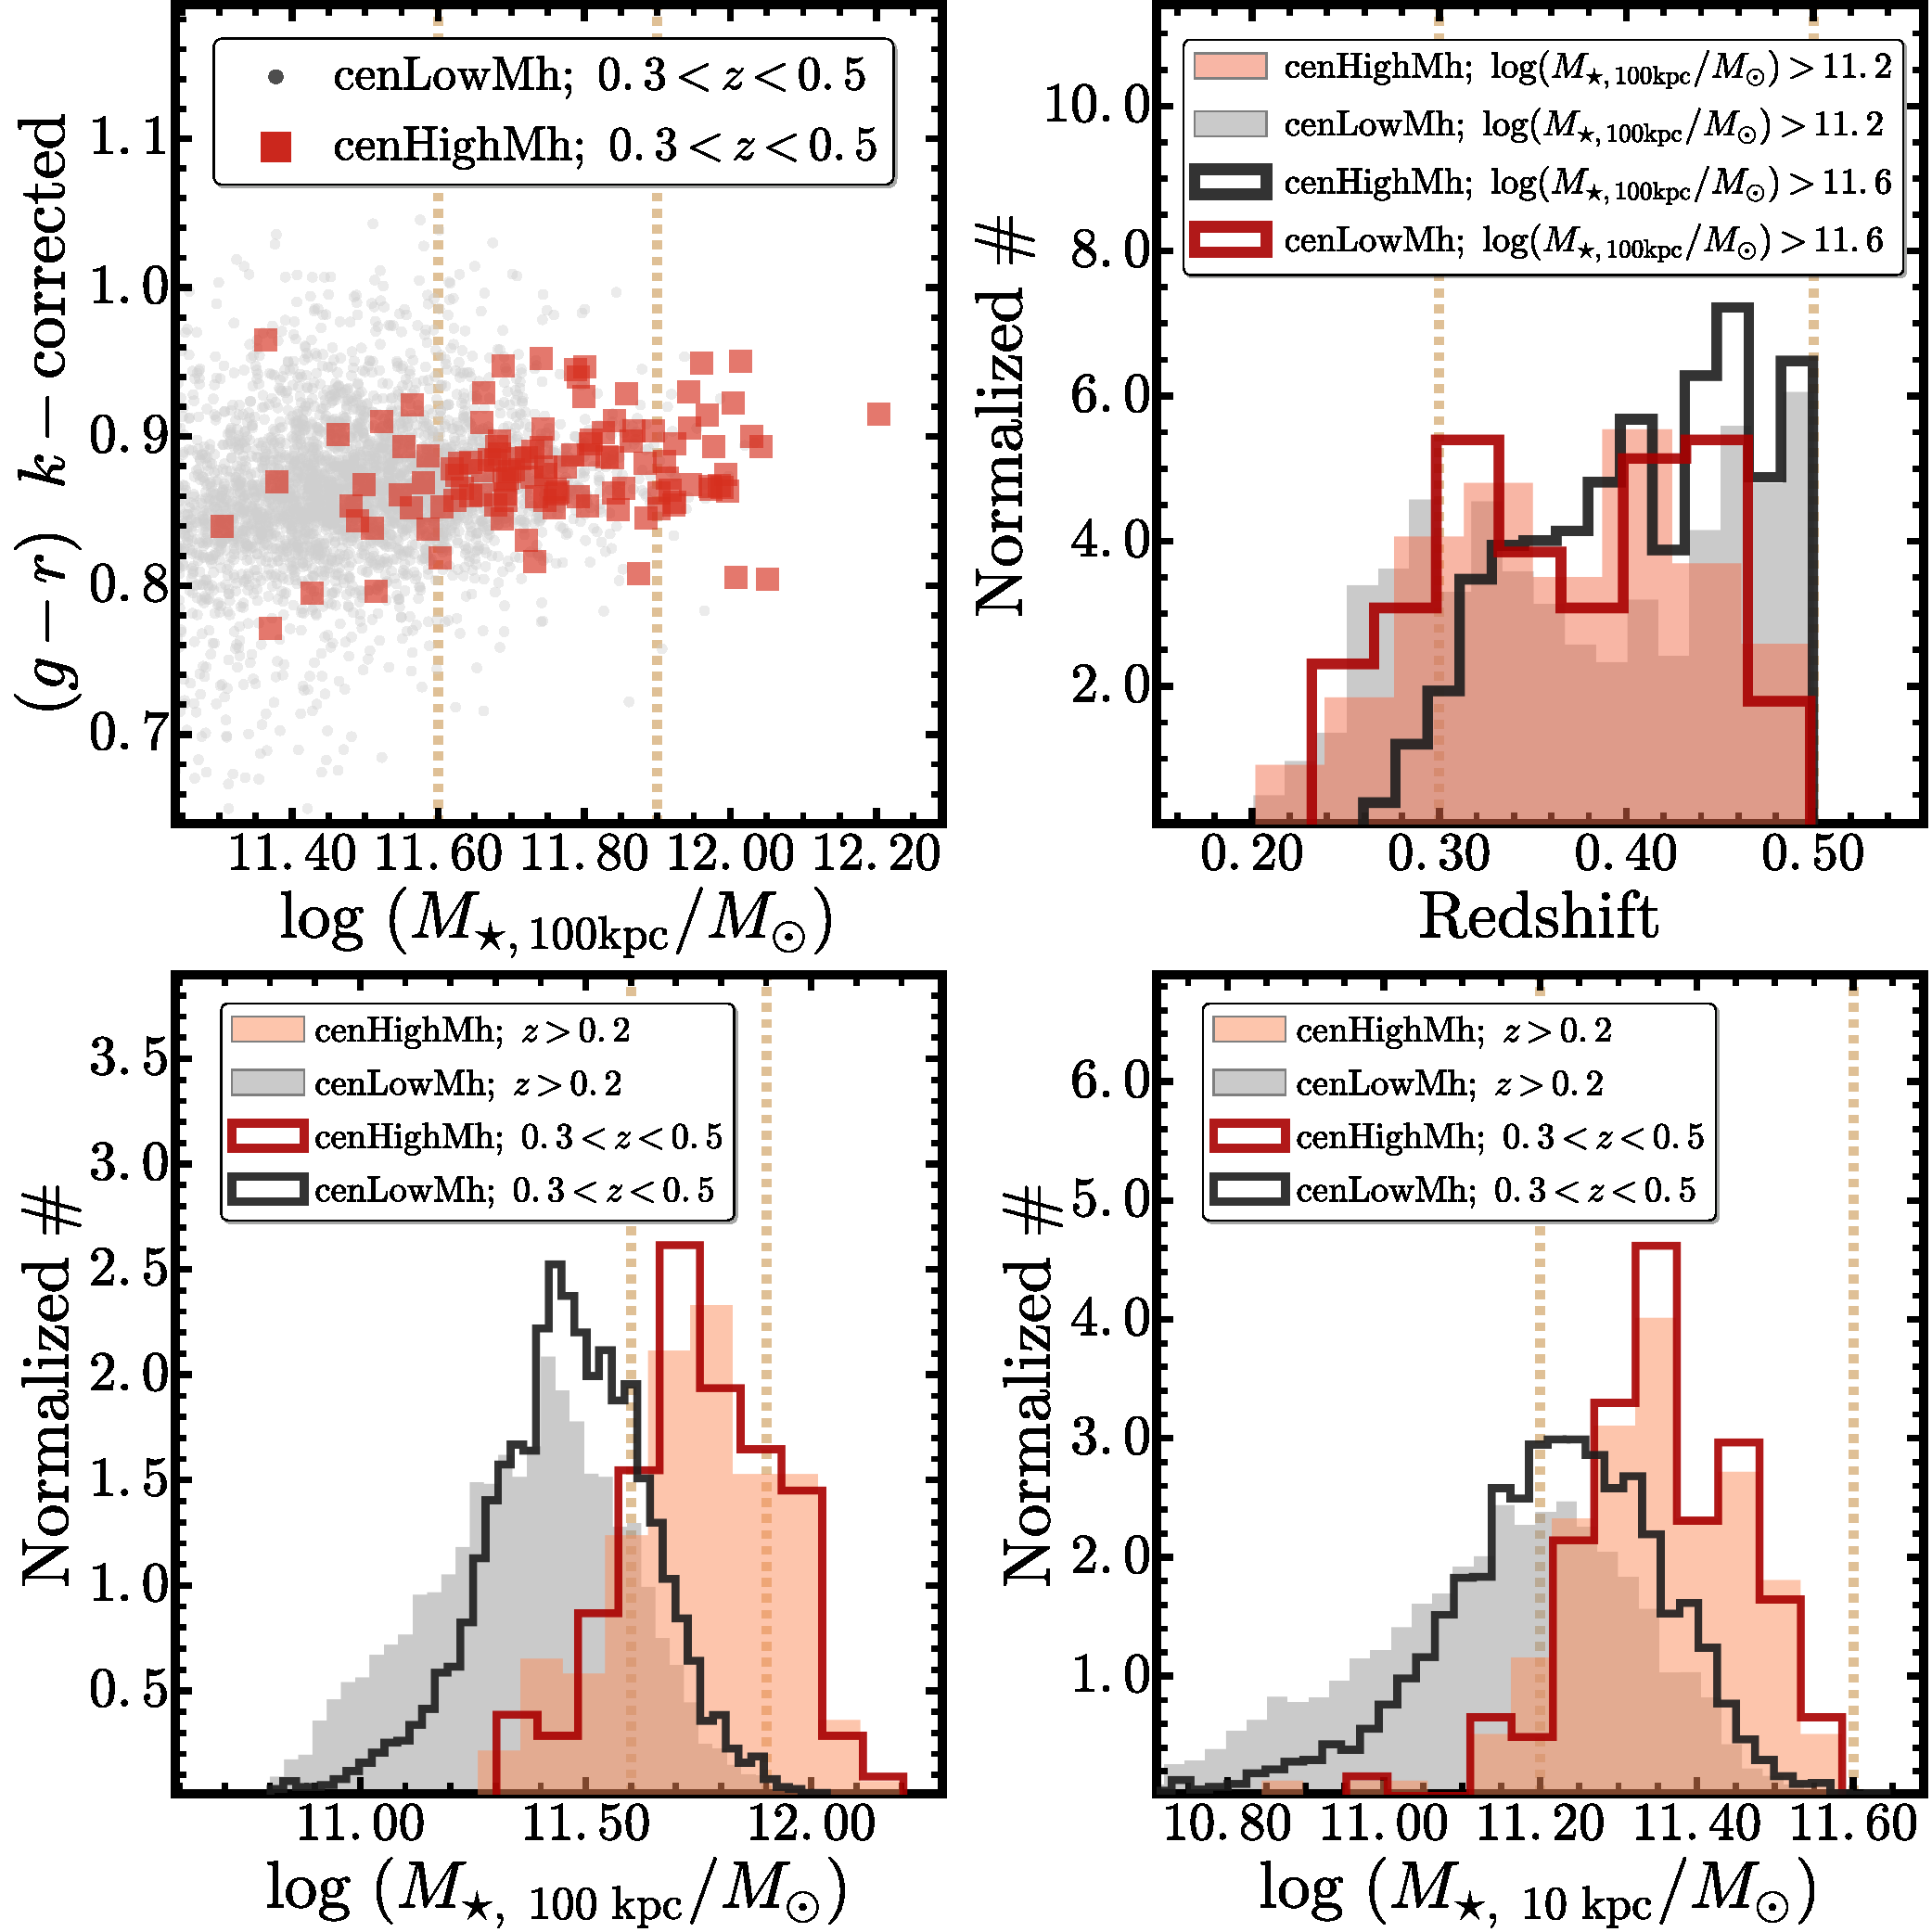
\includegraphics[width=16.5cm]{fig/redbcg_sample_stats}
      \caption{
          \update{
          \textbf{Top-left}: The \logms{}-$g-r$ color relation of the \rbcg{} 
          (red circle; detaield format is the same with the right panel of 
          Fig.\ref{fig:smf1}) and \nbcg{} (grey dots) samples.
          We apply the $k$-corrections from \texttt{iSEDFit} fitting to the colors.~~          
          \textbf{Top-right}: the histograms of the redshift for the \rbcg{} and 
          \nbcg{} galaxies in both \logmtot$>11.2$ and $11.6<$\logmtot{}$<11.9$
          mass bins.
          The vertical lines highlights the $0.3\leq z \leq 0.5$ redshift range.~~
          \textbf{Bottom-left}: the histograms of \mtot{} for the \rbcg{} (orange-red) 
          and \nbcg{} (grey-black) samples at both $z>0.2$ (step-filled histogram) and 
          $0.3 \leq z \leq 0.5$ (stepped histogram). 
          The vertical lines in both top-left and bottom-left figures highlight the 
          $11.6<$\logmtot{}$<11.9$ mass range that will be used in the comparison of 
          the \mtot{}-matched samples.~~
          \textbf{Bottom-right}: the histograms of \minn{} in similar format. 
          Here the vertical lines highlight the 
          $11.2<$\logminn{}$<11.6$ mass range that is used for comparison.}
      }
      \label{fig:sample_stats}
  \end{figure*}
%% ------------------------------------------------------------------------------------ %% 
    

\section{B. Extraction of 1-D surface brightness profile} 
    \label{app:A}
%% ------------------------------------------------------------------------------------ %% 
    \begin{figure*}[hbt!]
        \centering 
        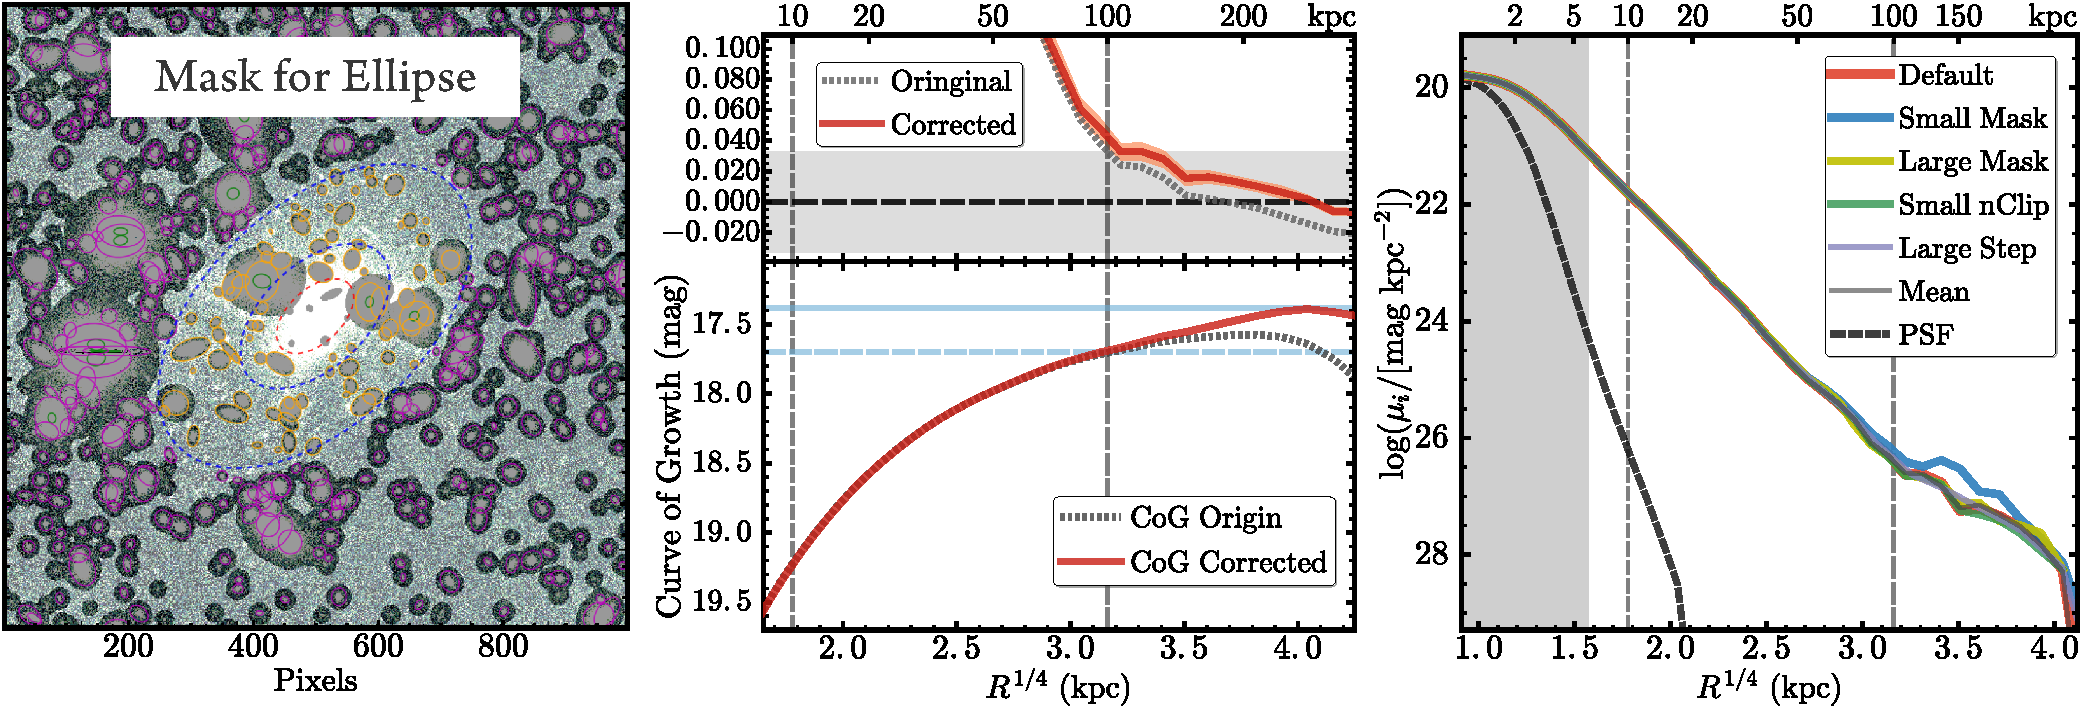
\includegraphics[width=\textwidth]{fig/redbcg_ellipse_tech}
        \caption{\textbf{Left:} Example of the object-mask built for the \texttt{Ellipse}
            run for a typical massive galaxy in the sample. 
            All the shaded regions are masked out. 
            The three dash lines (red, inner one and two blue ones) around the target 
            at the center outlines the three radius we defined using the flux radius 
            of the target.  
            We increase the mask size for objects detected in different regions 
            separated by these apertures (which are outlined by solid, elliptical 
            apertures with different colors) using slightly different criteria.~~
            \textbf{Middle:}: The flux profile that is zoomed into the near-zero flux 
            range (top panel), and the curve-of-growth of the magnitude for the example
            massive galaxy.  
            To highlight the importance of correcting sky background, we show the profiles 
            using both images with (red, solid line) and without (black, dash line) 
            ad-hoc background correction. 
            On the top panel, besides the horizontal line that highlights the zero flux 
            level, we also show the uncertainty of the sky background estimate via 
            grey-shaded region.  
            On the bottom panel, two horizontal lines indicate the magnitudes 
            corresponding to total (solid) and half flux (dash) using the 
            background-corrected profile. ~~
            \textbf{Right:} compare the 1-D surface brightness profiles for the same 
            example galaxy extracted using different mask 
            (smaller masking region: red, dash line; larger masks: blue, dash line), 
            or different \texttt{Ellipse} settings
            (more aggressive pixel-clipping: cyan, dash line; 
             larger step in radius: green, dash line; 
             using mean flux along the isophote instead of median: purple, dash line)
            with the one using the default configuration (black, solid line).}
            \song{Figure will be updated}
        \label{figure:A1}
    \end{figure*}
%% ------------------------------------------------------------------------------------ %% 

%% ------------------------------------------------------------------------------------ %% 

\section{C. Estimate average {$M_{\star}/L_{\star}$} using \texttt{iSEDFit}} 
    \label{app:B}

%% ------------------------------------------------------------------------------------ %% 
    \begin{figure*}[bt!]
        \begin{center}
        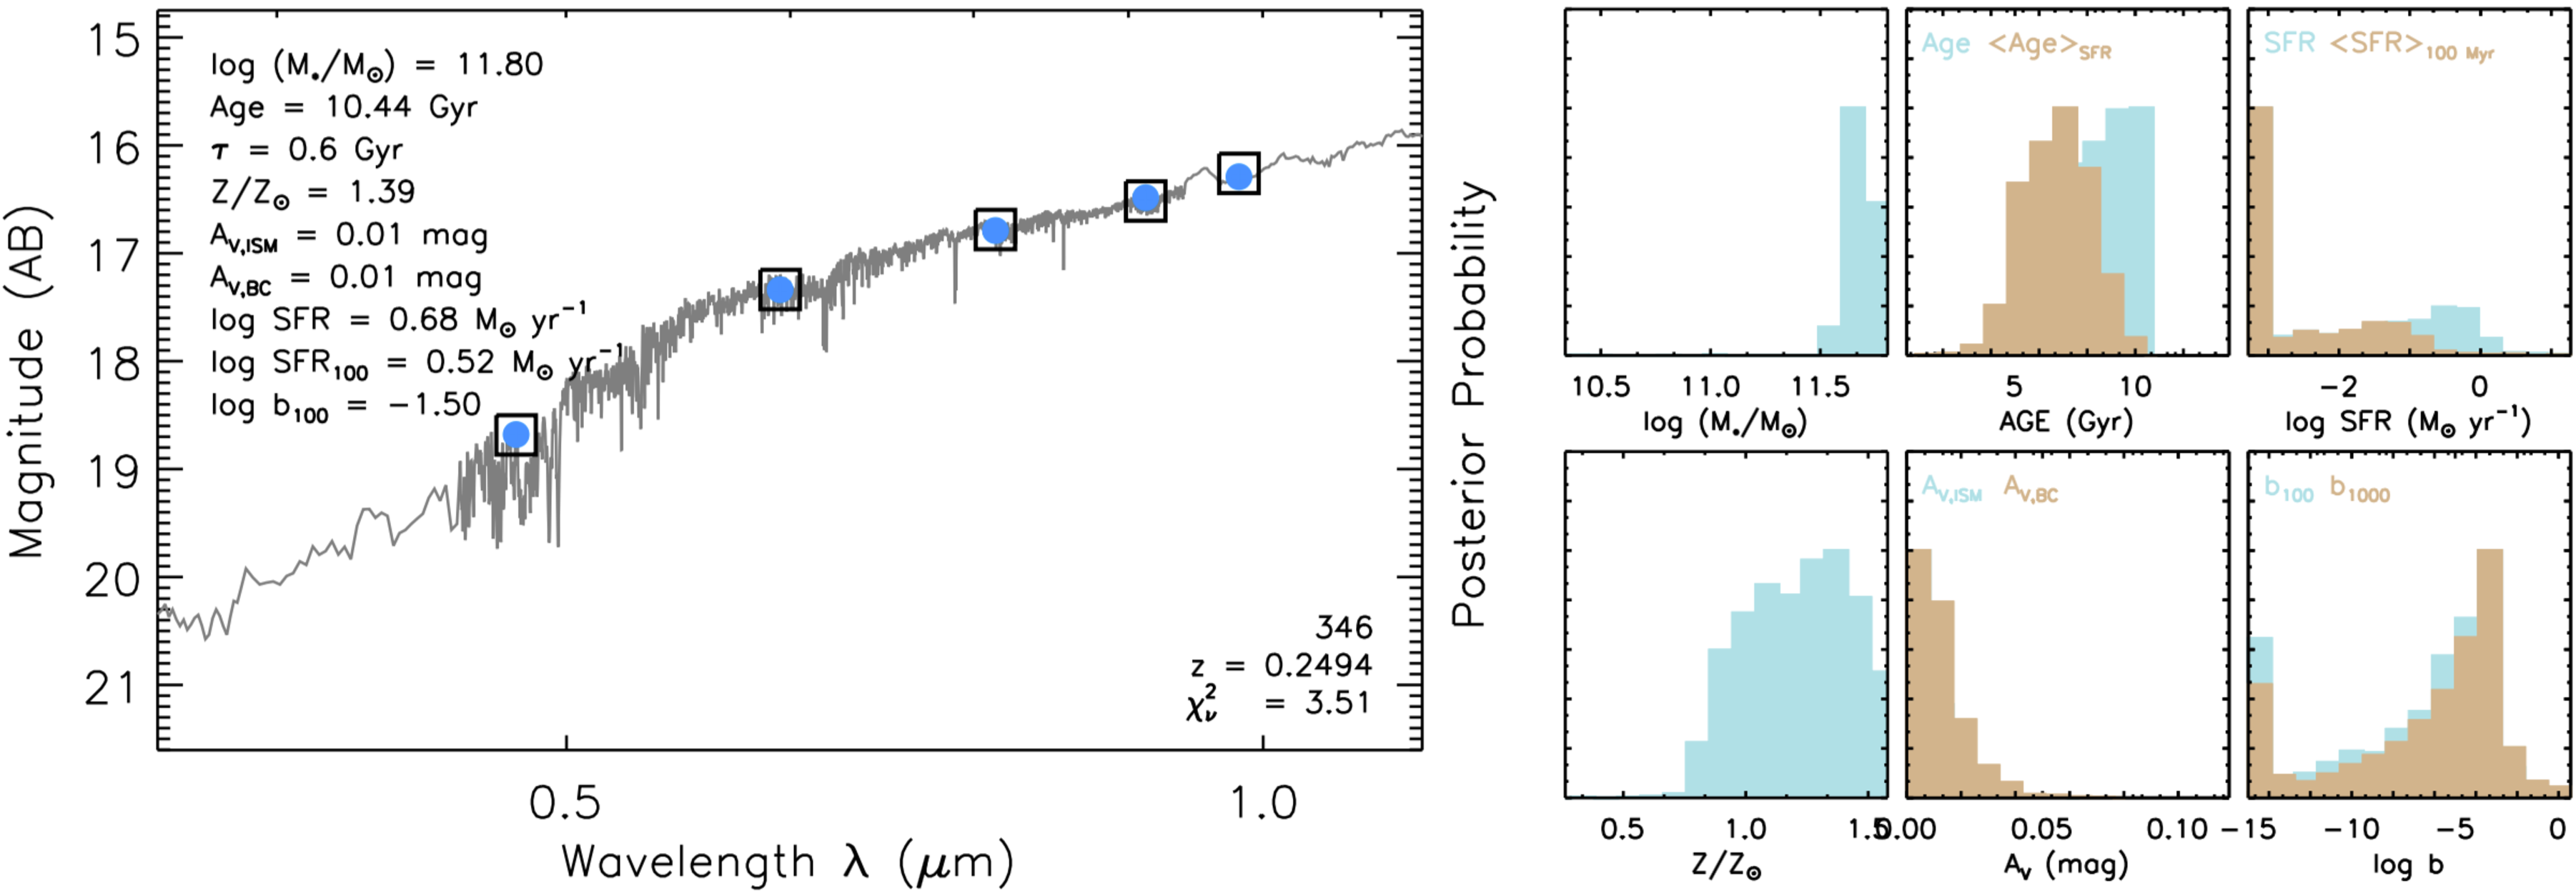
\includegraphics[width=\textwidth]{fig/redbcg_isedfit_example.pdf}
        \caption{Left: example output figure from \texttt{iSEDFit} that shows the SED 
        	fitting results. 
            The open-boxes show the observed fluxes in 5-band, and the solid, blue-dots
            show the best-fitted results, along with the high-resolution spectrum for
            this model recontructed using the synthetic spectra from \texttt{FSPS}. 
            Top-left corner shows the best-fit stellar population parameters, and 
            bottom-right corner shows the ID, redshift of this object, and reduced 
            $\chi^2$ of the best-fit model.~~~
            Right: the Posterior distributions of a few key parameters.
            From top-left to bottom right are: 1) stellar mass (\logms{}); 2) age of the 
            population (mass and star-formation rate weighted) in Gyr; 3) star formation 
            rate ($\log\ \mathrm{SFR}\ (M_{\odot}/\mathrm{yr})$; instant one and the one 
            averaged over the previous 100 Myr; 4) stellar metallicity 
            ($\mathrm{Z}/\mathrm{Z}_{\odot}$); 5) dust extinction ($\mathrm{A}_V$ in mag);
            6) birthrate parameter ($\log\ b$; averaged over previous 100 and 1000 Myr).}
        \label{fig:ised}
        \end{center}
    \end{figure*}
%% ------------------------------------------------------------------------------------ %% 

%% ------------------------------------------------------------------------------------ %% 
    \begin{figure*}[hbt!]
        \begin{center}
        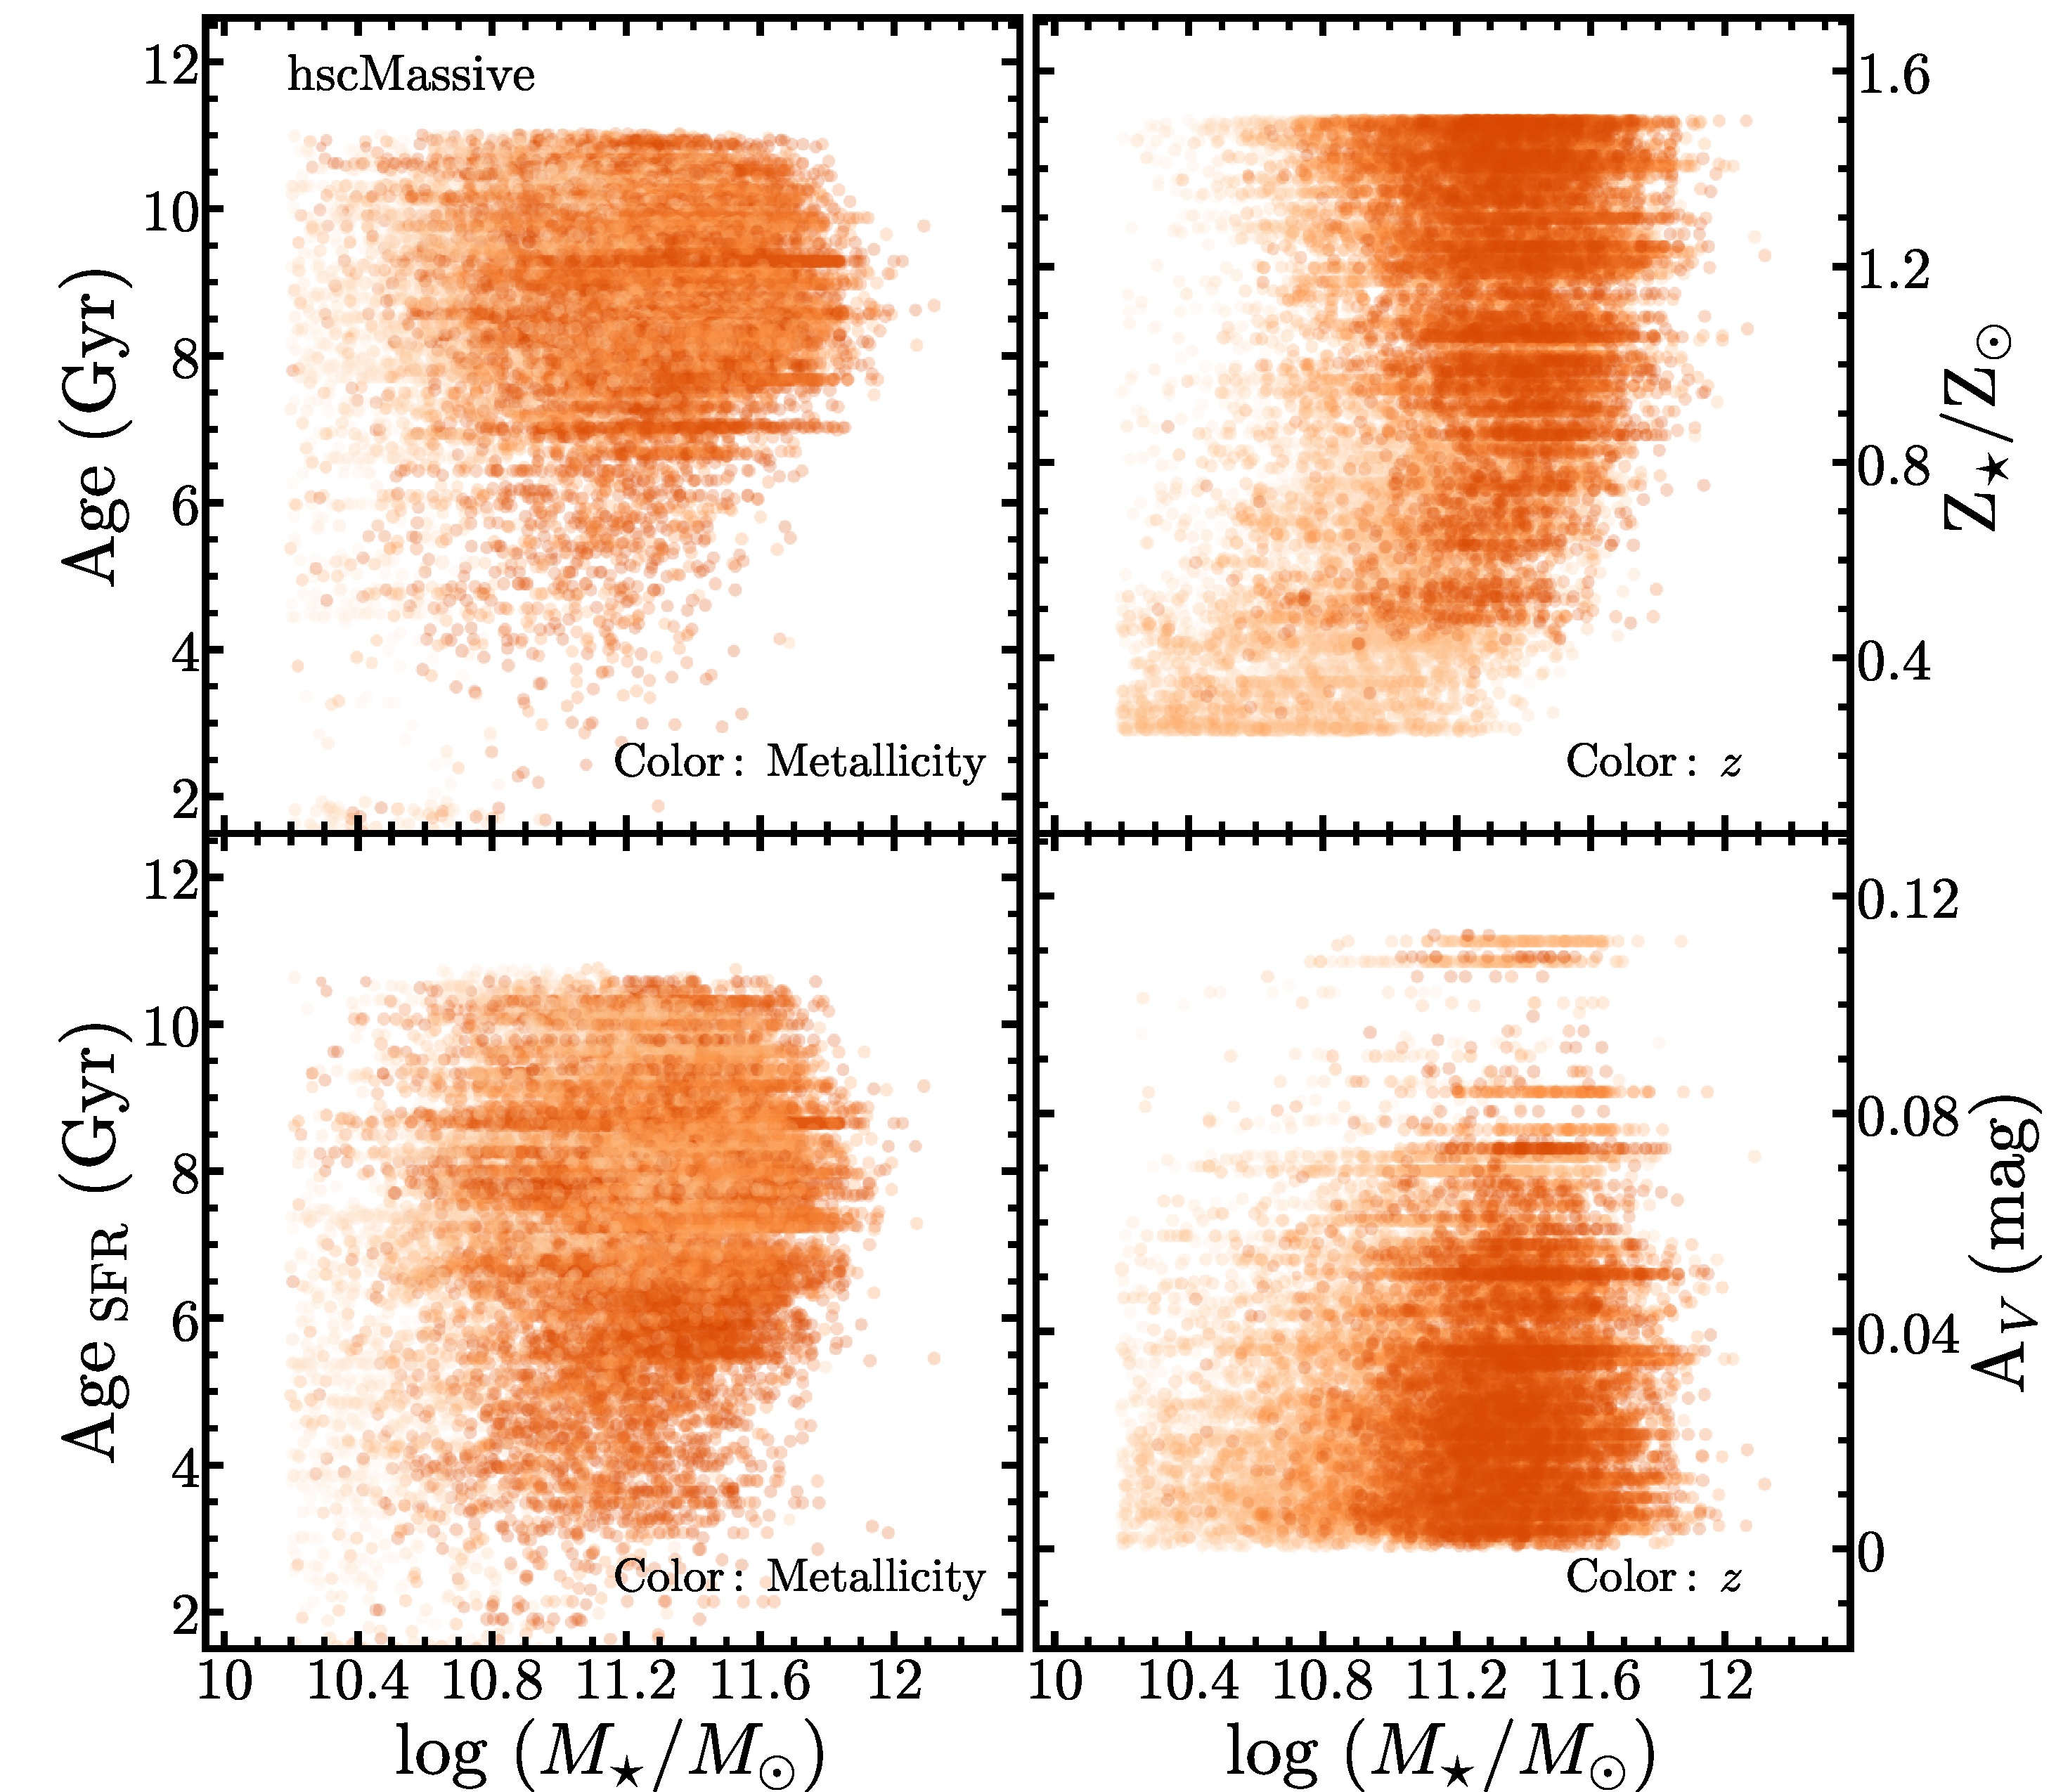
\includegraphics[width=\textwidth]{fig/redbcg_isedfit_2.pdf}
        \caption{Relationships between \mstar{} and certain stellar population 
            parameter using \texttt{iSEDfit}. 
            The left figures are for the \rbcg{} sample, while the right ones are 
            for the \nbcg{} sample. 
            They are both color-coded using the mass-weighted stellar age. 
            The four stellar population properties shown here are: 
            1) mass-weighted stellar age in Gyr (top-left); 
            2) SFR-weighted stellar age in Gyr (bottom-left); 
            3) mass-weighted stellar metallicity in unit of solar value (top-right);
            4) dust extinction value in magnitude (bottom-right).}
        \label{fig:ised_2}
        \end{center}
    \end{figure*}
%% ------------------------------------------------------------------------------------ %% 

%% ------------------------------------------------------------------------------------ %% 
    \begin{figure*}[hbt!]
        \begin{center}
        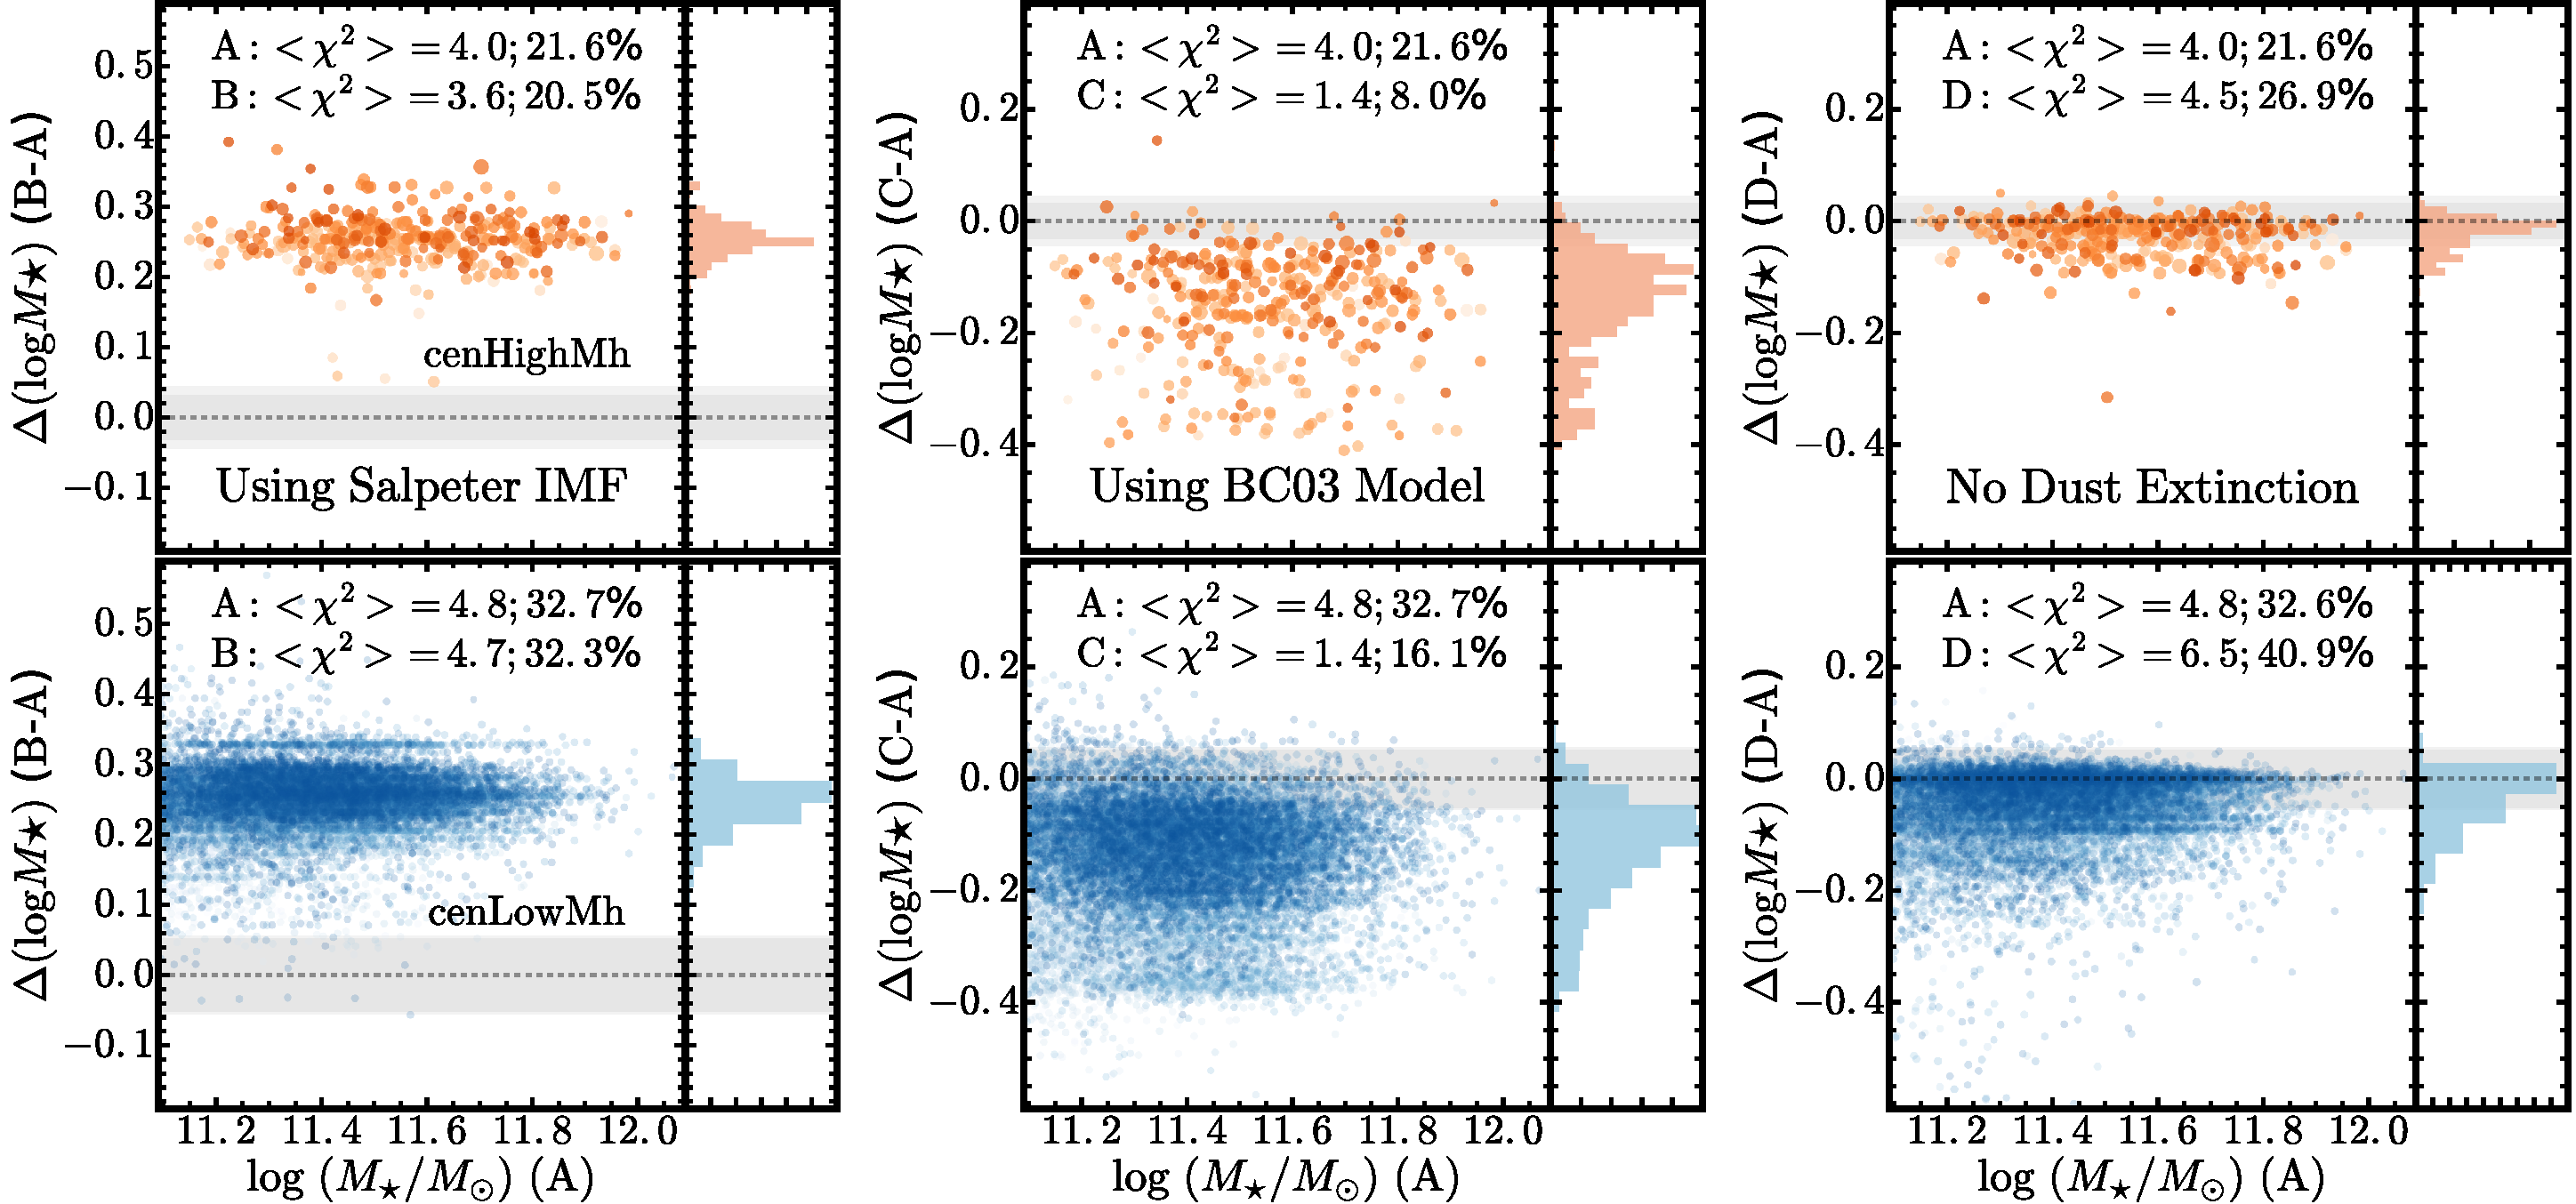
\includegraphics[width=\textwidth]{fig/redbcg_isedfit_3.pdf}
        \caption{Comparisons of \mstar{} estimated by \texttt{iSEDFit} using different
            assumptions. 
            In each figure, we plot the default \mstar{} values against their 
            differences with the results using other models. 
            The top (bottom) row shows comparisons for the \rbcg{} (\nbcg{}) sample. 
            The results involved here are labeled: 
            (A): default one; 
            (B): using the Salpeter IMF instead of the Chabrier one (Left column);
            (C): using the BC03 synthetic population model instead of the FSPS one
                 (Middle column);
            (D): assume that there is no dust extinction (Right column). 
            On each figure, a horizontal line shows the zero difference level, along
            with the grey shaded region that highlights the typical uncertainty of 
            the \mstar{}-differences. 
            We also show the histogram of the \mstar{}-differences on the right.}
        \label{fig:ised_3}
        \end{center}
    \end{figure*}
%% ------------------------------------------------------------------------------------ %% 

    We adopt flat distribution between 0.5 to 14.0 Gyrs as prior for the look-back 
    time when the star formation turned on. 
    The exponential delayed time-scale ($\tau$) is allowed to change between 
    0.1 to 3.0 with equal probability.  
    The chance of random star burst is set at 0.2 for every 2 Gyrs. 
    The duration of the star burst is draw from a logarithmic distribution 
    between 0.03 to 0.3 Gyr; and the mass fraction formed in the burst is from 
    a logarithmic distribution between 0.01 and 1.0.  

    In principle, these choices of priors could leave systematic effects in 
    the estimate of stellar mass (e.g.\ \citealt{Bernardi2016b}). 
    For low-$z$ massive ETGs like the ones in our sample, the details form of 
    SFH, importance of random star burst, and the dust extinction should not be 
    major concern.  
    However, the choices of stellar population models and IMF can still 
    change the results systematically. 
    More discussions on this can be found in Appendix~A. 
    In short: 
    \begin{enumerate}
        \item Both \texttt{FSPS+MILES} and \texttt{BC03} (\citealt{BC03} models 
            still have difficulties recovering the optical color involving filters 
            at the red end (e.g~$i-$Y), which could relate to the challenge for 
            modern stellar population models to reproduce the optical color-color 
            relation of red-sequence galaxies (e.g.\ \citealt{MIUSCAT2}), or the 
            shallower photometry of HSC-Y band data. 
        \item The \texttt{BC03} provides slightly better overall ${\chi}^2$ and 
            systematically smaller \mstar{} than the \texttt{FSPS+MILES} models.  
            However, it is possible that the \texttt{BC03} model tends to 
            underestimate the \m2l{} for a fraction of them as the estimate 
            stellar age is unrealistically young for red, massive galaxies.  
            Therefore, we still use the \texttt{FSPS+MILES} model as the fiducial 
            one.  But, switching to the \texttt{BC03} model will not change any 
            key result in this work. 
        \item The usage of \citet{Salpeter1955} IMF results in systematically 
            higher \mstar{} (on average $+0.25$ dex of \logms{}).  
            Although there are multiple lines of evidence that favor Salpeter 
            or even more ``bottom-heavy'' IMF in the most massive ETGs 
            (e.g.\ \citealt{Conroy2012}; \citealt{Cappellari2012}), we still 
            present the main results using Chabrier IMF to accommodate galaxies 
            with lower \mstar{} in the sample, and to be as consistent as possible 
            with a few other works.  
            Also, the choice of IMF does not impact our results qualitatively.     
    \end{enumerate}
    
    Besides the priors for stellar population properties, different treatments of 
    the light profile and accuracy of sky background subtraction are also important
    for the estimate of \mstar{} as they strongly impact the estimate of total luminosity
    (e.g.\ \citealt{Bernardi2013} and \citealt{DSouza2015}).  
    At the depth of SDSS, the default \texttt{cModel} photometry is already shown to 
    be not very accurate at high-\mstar{} end (e.g.\ \citealt{Meert2015}; 
    \citealt{Bernardi2016a}) as it does not capture the extended envelope of these 
    galaxies. 
    As for HSC, it is much more challenging for \texttt{cModel} to recover the total 
    luminosity of massive ETGs since the stellar envelope becomes even more 
    extended for neither de~Vaucouleur or exponential model to reproduce.  
    However, the HSC \texttt{cModel} under the force-photometry mode can measure 
    \textbf{average} color of the galaxy with great accuracy (e.g.\ Huang\etal~in prep.~), 
    and provide us a reliable SED to estimate the \textbf{average} \m2l{}. 
    Considering this, we separate the process of estimating the total \mstar{} of 
    massive ETGs in our sample into two steps: 
    
    \begin{enumerate}
        \item Firstly, using the redshift and \texttt{cModel} magnitude in five bands, 
            we derive an initial estimate of the \mstar{} of the galaxy.  
            More importantly, we derive the \textbf{average} \m2l{} in $i$-band of the 
            galaxy, and use the best-fit SED to provide $k$-correction to the photometry.  
        \item In the next section, we will derive better estimate of total \mstar{} using 
            the more accurate total luminosity in $i$-band from integration of carefully 
            measured 1-D surface brightness profile, and the average \m2l{} from the SED
            fitting.  
    \end{enumerate}
    
    The basic results from \texttt{iSEDFit} are summarized in Figure~2, where we compare
    the relations between initial estimates of \mstar{} and (both luminosity and 
    star formation weighted) stellar age, metallicity, and dust extinction. 
    As expected, most galaxies in our samples are 
    $\log(M_{\star,\ \mathrm{ini}}/M_{\odot}) \geq 11.2$ massive galaxies that have 
    old age, high metallicity ($1.5 \times Z_{\odot}$ is the highest metallicity allowed), 
    and low dust extinction.  
    Given that we only have photometry from five optical bands, degeneracies among 
    age, metallicity, and dust extinction are naturally expected.  
    We will not use them for any scientific reason in this work, but to show that they
    behave reasonably.   

%% ------------------------------------------------------------------------------------ %% 

\section{D. Comparison of \mden{} profiles using \mstar{} from the GAMA survey}
    \label{app:C}

%% ------------------------------------------------------------------------------------ %% 
\begin{figure*}[hbt!]
    \centering 
    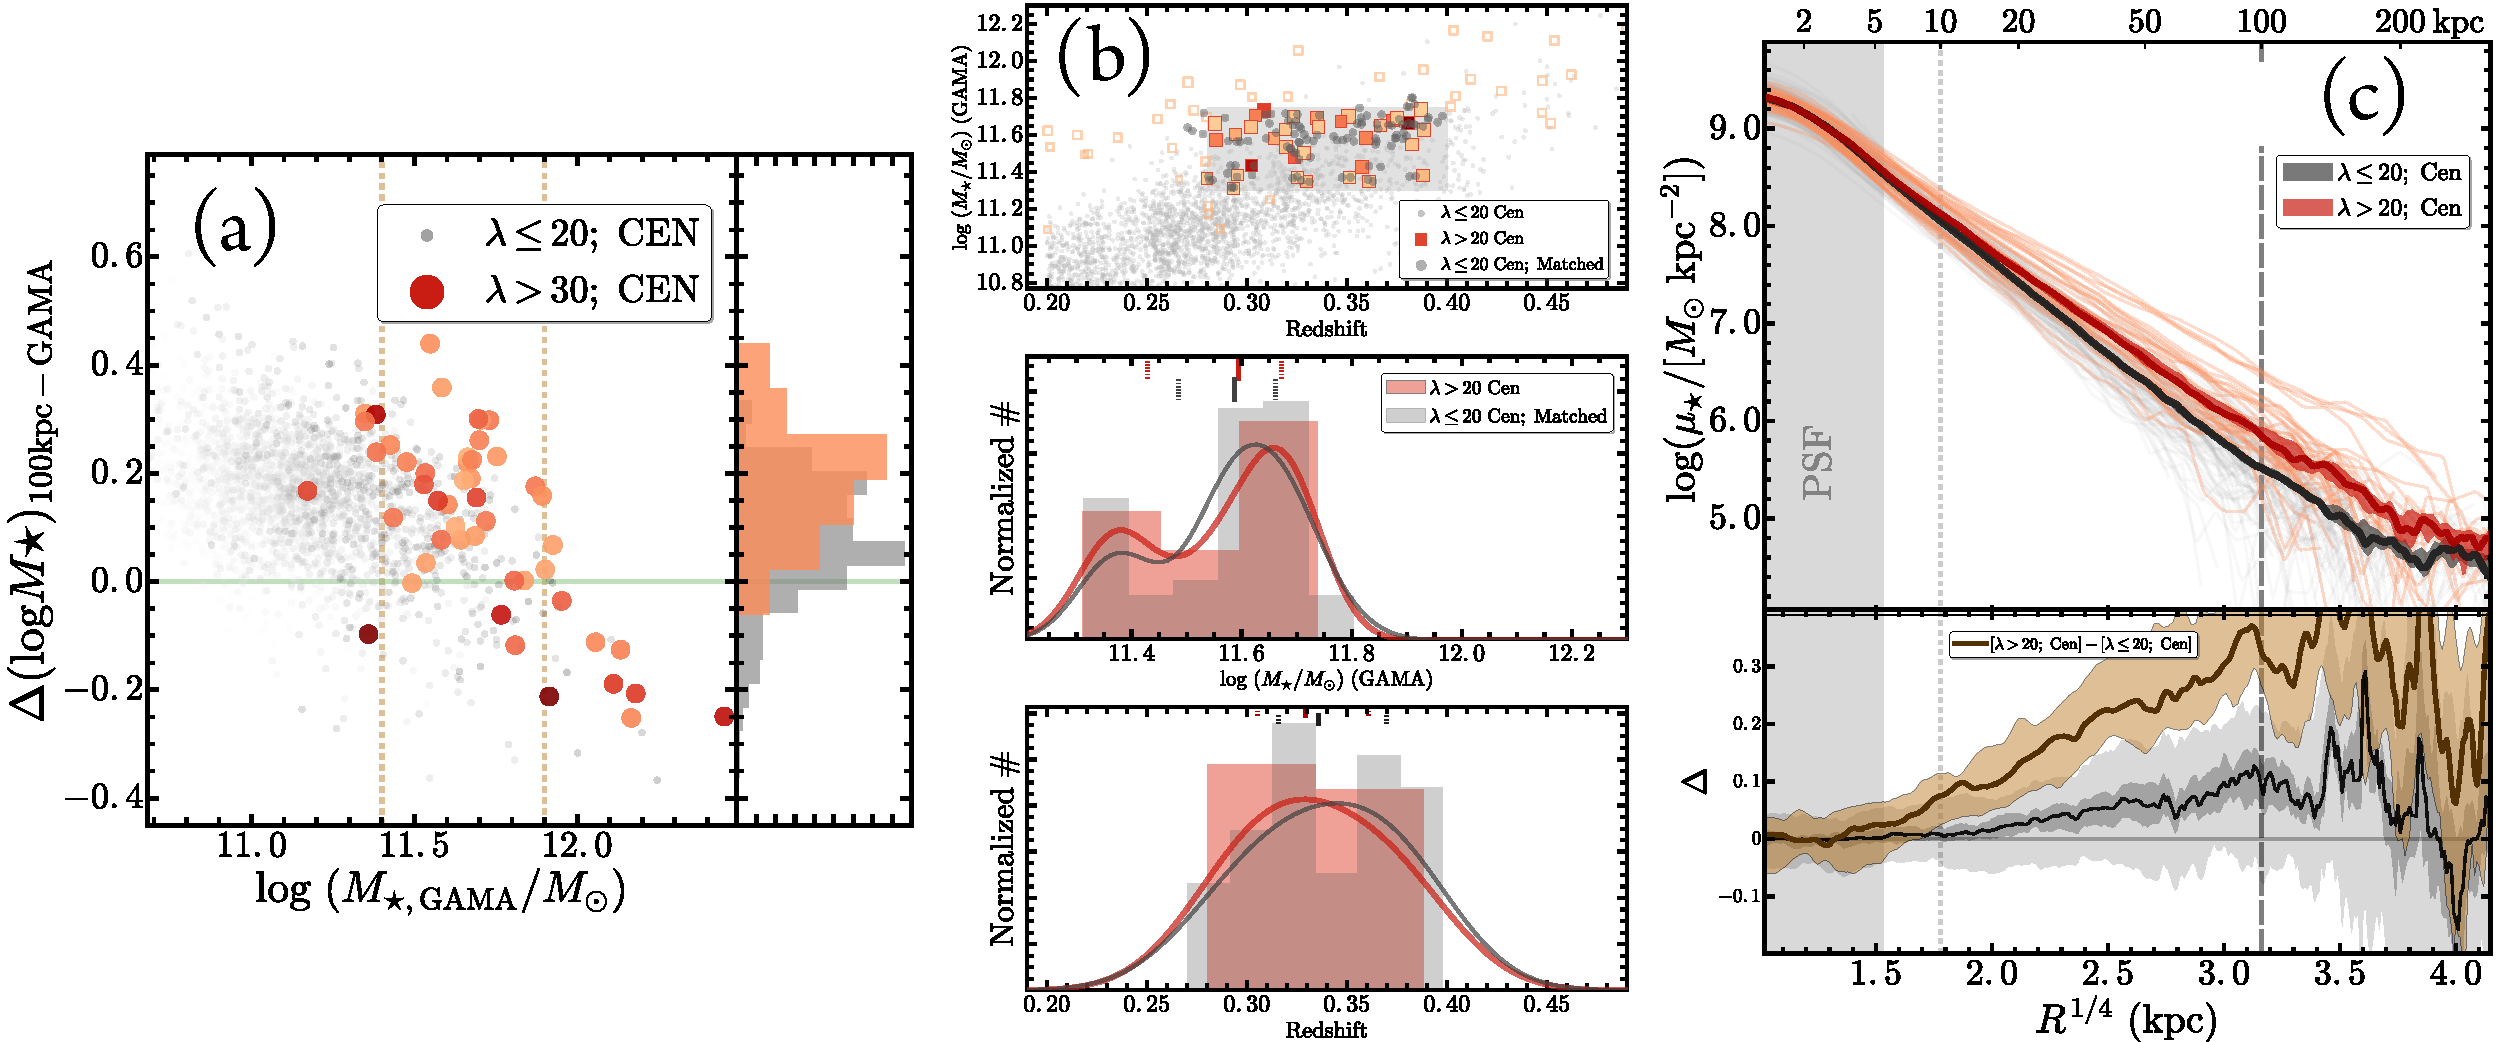
\includegraphics[width=\textwidth]{fig/redbcg_prof_gama_new}
    \caption{
        \update{
        \textbf{Left:} comparison of \mstar{} estimated by the GAMA survey and 
        the \mtot{} using HSC images in this work. 
        We plot the \logmgama{} against the difference between \logmtot{} and \logmgama{}. 
        The format is very similar to the left panel of Fig.\ref{fig:smf1}. 
        The two vertical lines highlight the mass range $11.4 \leq$\logmgama{}$<11.8$ 
        that is used for the comparison.~~
        \textbf{Right:} we compare the \mden{} profiles of \rbcg{} (orange-red) and 
        \nbcg{} (grey-black) galaxies using the samples matched on the 
        \mgama{}-$z$ plane at $11.4 \leq$\logmgama{}$<11.9$ and $0.28 \leq z < 0.4$. 
        The format is very similar to the ones in Fig.\ref{fig:prof_1}.}
        }
    \label{fig:gama}
\end{figure*}
%% ------------------------------------------------------------------------------------ %% 

    As the sky coverage of this release greatly overlaps with the GAMA survey,
    we start the detailed comparison with an external check using the stellar
    mass estimated by \citep{Taylor2011}. 
    The purpose is still to investigate the impact of deeper photometry on 
    the analysis of structure of massive galaxies.  
    The stellar masses of GAMA galaxies are initially derived through careful 
    optical-SED fitting (BC03 model; Chabrier IMF) using the PSF-matched 
    aperture photometry.  
    Then they were corrected for the total luminosity estimated using single-\ser{}
    2-D model to multi-band images (\citealt{Kelvin2012}).  
    We separate the \rbcg{} and \nbcg{} galaxies that also have 
    spec-$z$ and stellar mass in GAMA DR2 (\citealt{Liske2015}).
    Most of galaxies in these subsamples have $z < 0.40$. 
    
    % Move the section about matching to Mtot matched section
    
    In Fig.~10, we show the results of matches for subsamples using 
    $M_{\star, \mathrm{GAMA}}$.  
    To increase the number of available \rbcg{} to match, we loosen 
    its selection criteria to $\lambda \ge 20$ and $P_{\mathrm{CEN}} \ge 0.6$.
    Based on the distributions of the two samples at the $M_{\star, \mathrm{GAMA}}$-$z$ 
    plane, and their overlapped region, we match them in two bins of 
    $M_{\star, \mathrm{GAMA}}$ that have slightly different redshift ranges. 
    %% moved
    For the samples in two $M_{\star, \mathrm{GAMA}}$, the matches appear to be
    very good.  
    
    In Fig.\ref{fig:gama}, we show the individual profiles, median profiles along with their 
    uncertainties derived using 5000 times bootstrap resampling, and the relative 
    difference between the profile of the \rbcg{} and \nbcg{} 
    subsamples.  
    It is very clear that, for both mass bins, the \rbcg{} has a much 
    more extended outer envelope, while its profile inside $\sim 10$ kpc is 
    very close to the \nbcg{} one.  
    This is inconsistent with the matched distributions of their ``total'' 
    stellar mass, and reveals potential issue with the stellar mass estimated 
    by GAMA.
    We can reproduce very similar results using the luminosity density profiles 
    (with or without $k$-correction) of these matched samples, which suggests 
    that the main problem does not lie in the estimate of \m2l{}, but in the 
    measurement of total luminosity using single-\ser model.  
    This highlights the importance of deep optical images in studying the 
    structure of massive galaxies. 
    
        In cases of these $M_{\star, \mathrm{GAMA}}$-matched samples, the differences
    of median profiles are very robust. 

%% ------------------------------------------------------------------------------------ %% 

\section{E. Comparisons of \mden{} profiles in different redshift bins}
    \label{app:D}

%% ------------------------------------------------------------------------------------ %% 
\begin{figure}[htb!]
    \centering 
    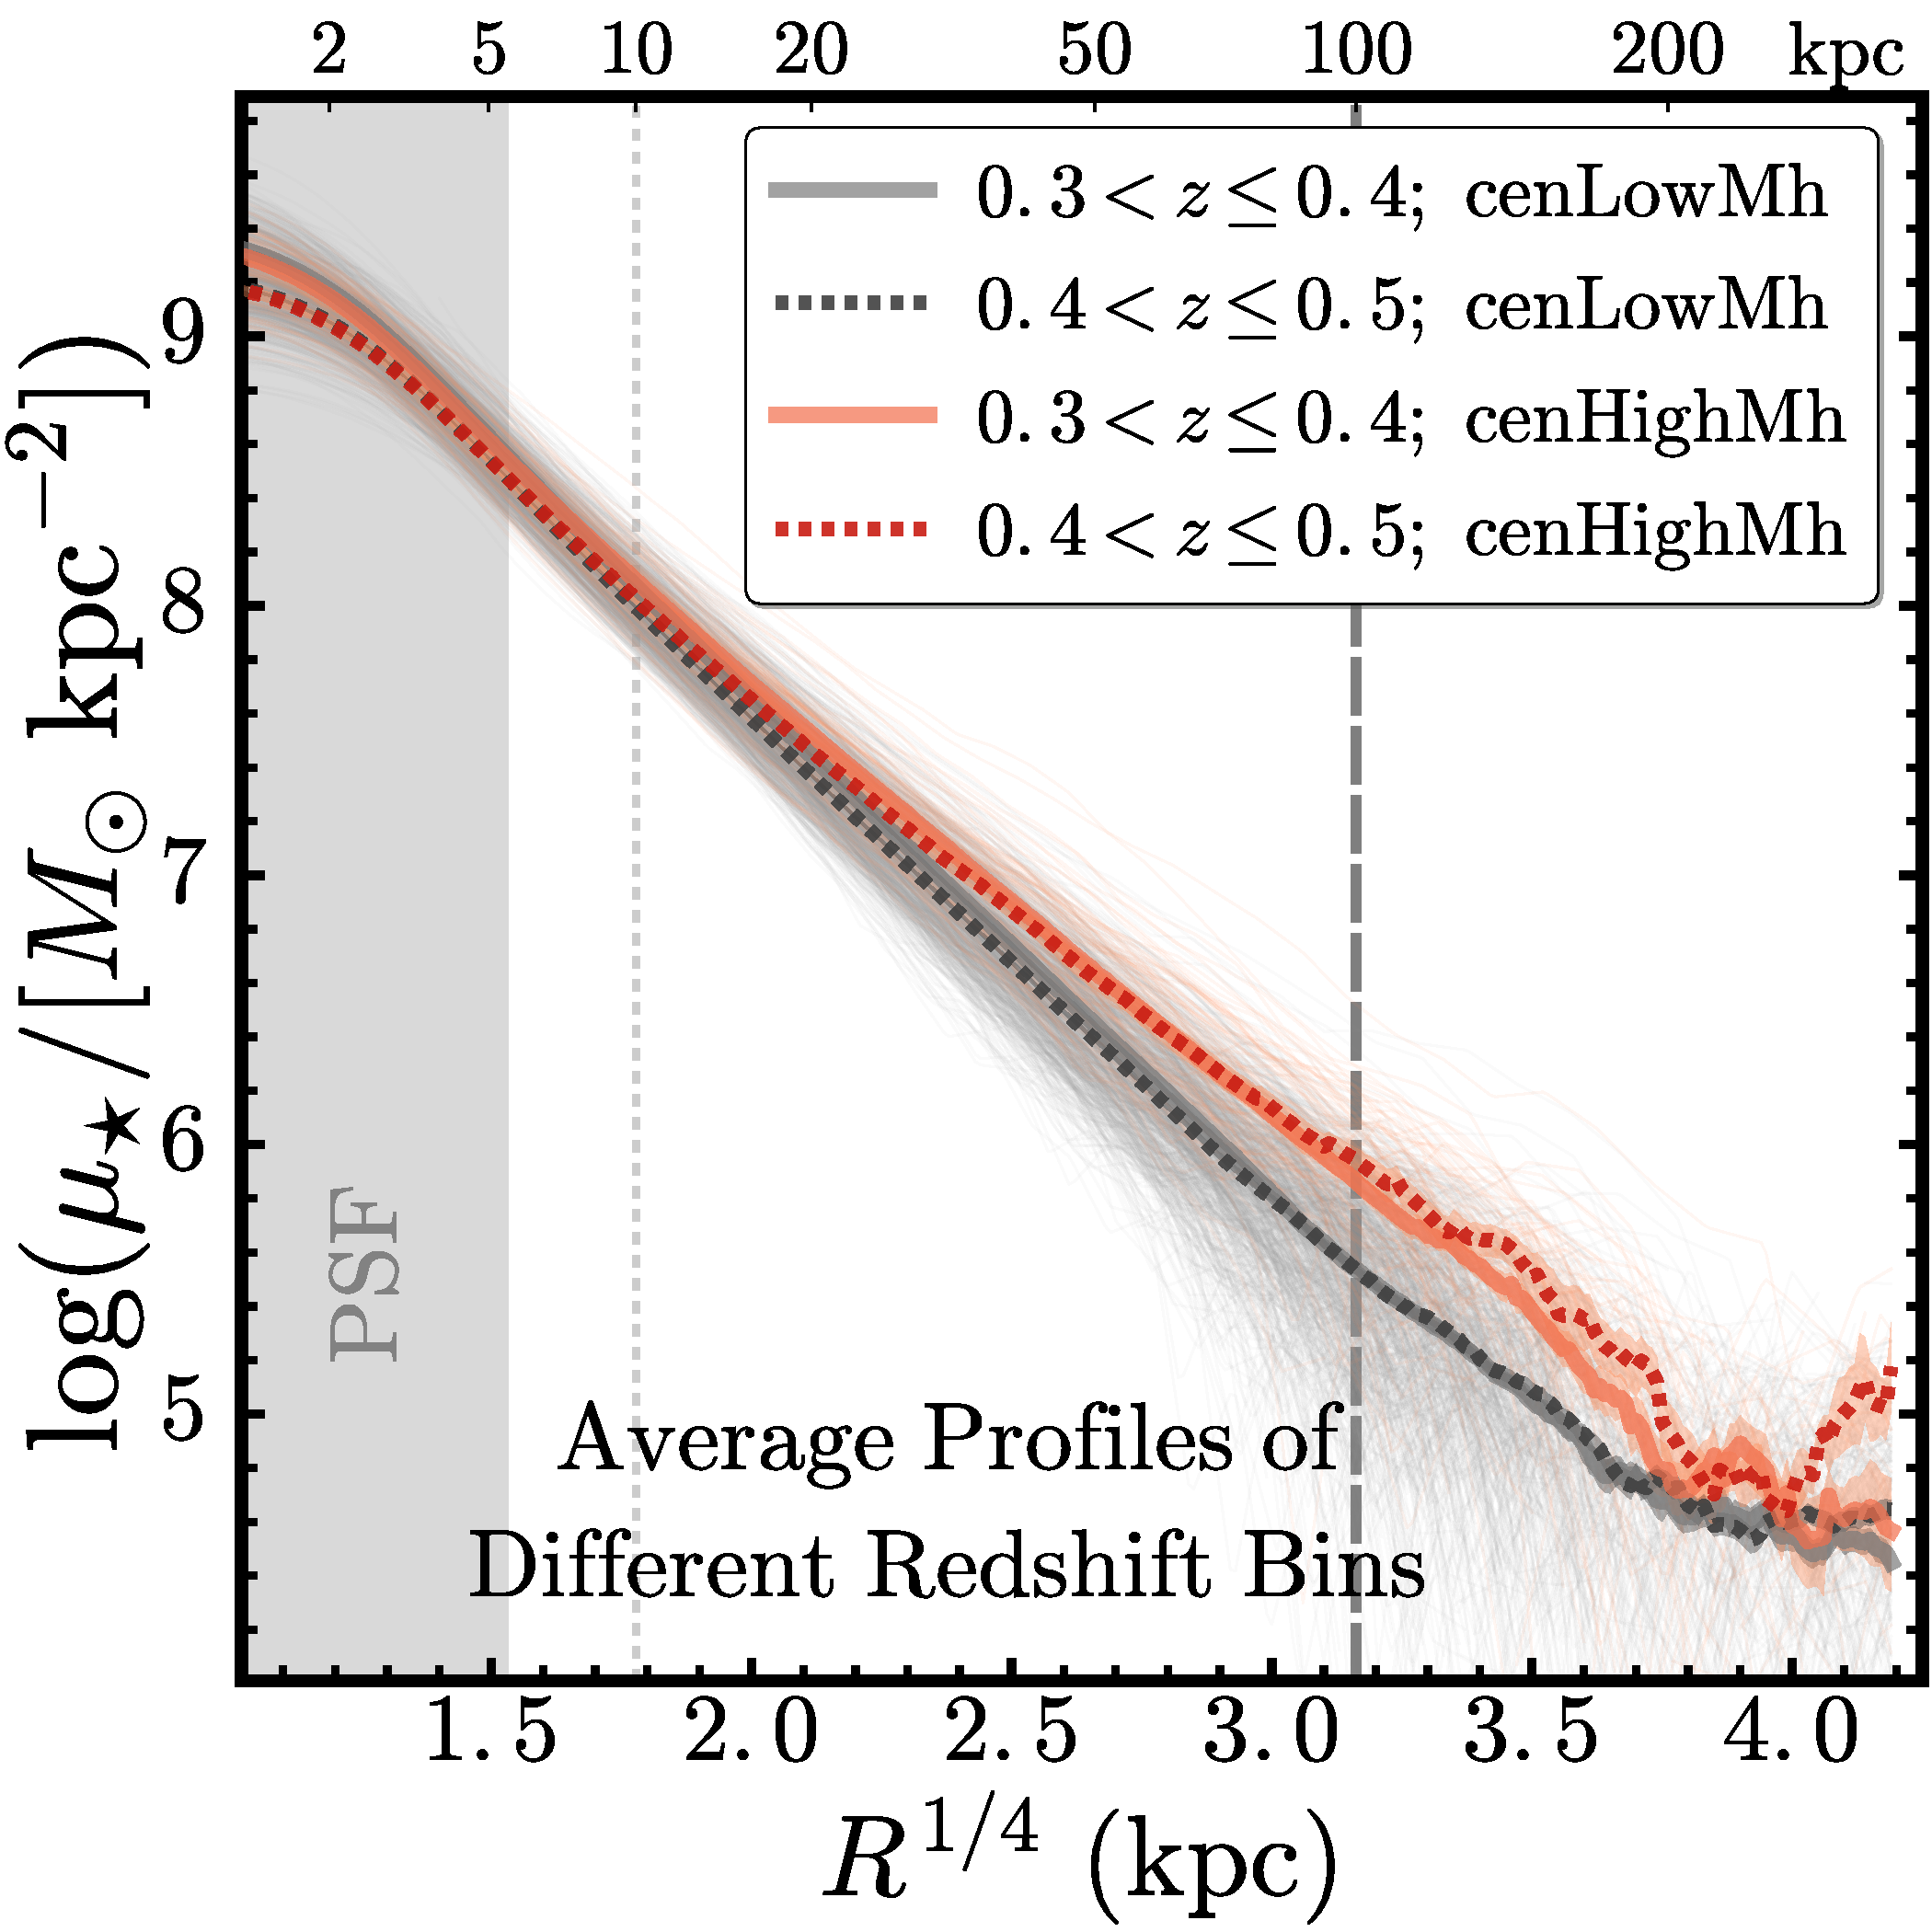
\includegraphics[width=13.0cm]{fig/redbcg_avg_prof_z}
    \caption{Comparison of \mden{} profiles of \rbcg{} (orange-red) and \nbcg{} 
        (grey-black) at $11.6 \le$\logmtot$< 11.9$ in redshift bins of 
        $0.3\leq z<0.4$ (solid lines) and $0.4\leq z<0.5$ (dash lines). 
        We show the individual profile in the background using much thinner line, 
        and highlight the median profiles using thicker line and darker color.
        Other formats are exactly the same with the left figure of 
        Fig.\ref{fig:avg_prof}.}
    \label{fig:D1}
\end{figure}    
%% ------------------------------------------------------------------------------------ %% 
    
    As the massive galaxies in our samples span quite a bit in both redshift and \mtot{}, 
    it is important to evaluate the impact from PSF on the \mden{} profiles at different 
    redshift. 
    In Fig.\ref{fig:D1}, we group the \rbcg{} and \nbcg{} galaxies at  
    $11.6 \le$\logmtot$< 11.9$ into two $z$ bins ($0.3\leq z<0.4$ and 
    $0.4\leq z<0.5$). 
    We did not match the \mtot{} distributions in two $z$ bins, so slight difference in 
    average \mtot{} can be expected. 
    With the same seeing condition, the \mden{} profile of galaxy at higher redshift is 
    more vulnerable to the PSF smearing effect in the center, while suffers more in the 
    outskirt due to cosmological dimming and background noise.  
    Fig.\ref{fig:D1} clearly shows that, although the median profiles of the same sample 
    in two redshift bins follow each other well outside 10 kpc, they start to differ in 
    the central 2-3 kpc as the one from higher redshift bin has more flattened profile 
    due to PSF smearing effect.  
    Meanwhile, we notice that the median profiles of \rbcg{} and \nbcg{} in the 
    same $z$ bin are very similar to each other in the region affected by seeing.   
    This comparison confirms the radius range that is sensitive to seeing and 
    redshift distribution is well constrained within the grey-shaded area.
    It also suggests that it is important to match the redshift distributions between 
    samples before we can compare their \mden{} profiles or other properties at inner 
    region, as we did in this work. 
    In the outskirt, within 100-150 kpc, we see no difference in the median \mden{} 
    profiles caused by redshift distributions. 
    We therefore conclude that it is safe to study the \mden{} profile within this 
    radius range for massive galaxies at $z<0.5$ using HSC images. 

\section{F. Match the \rbcg{} and \nbcg{} samples in \mstar{} and redshift distributions}
    \label{app:match}

%% ------------------------------------------------------------------------------------ %% 
\begin{figure*}[hbt!]
    \centering 
    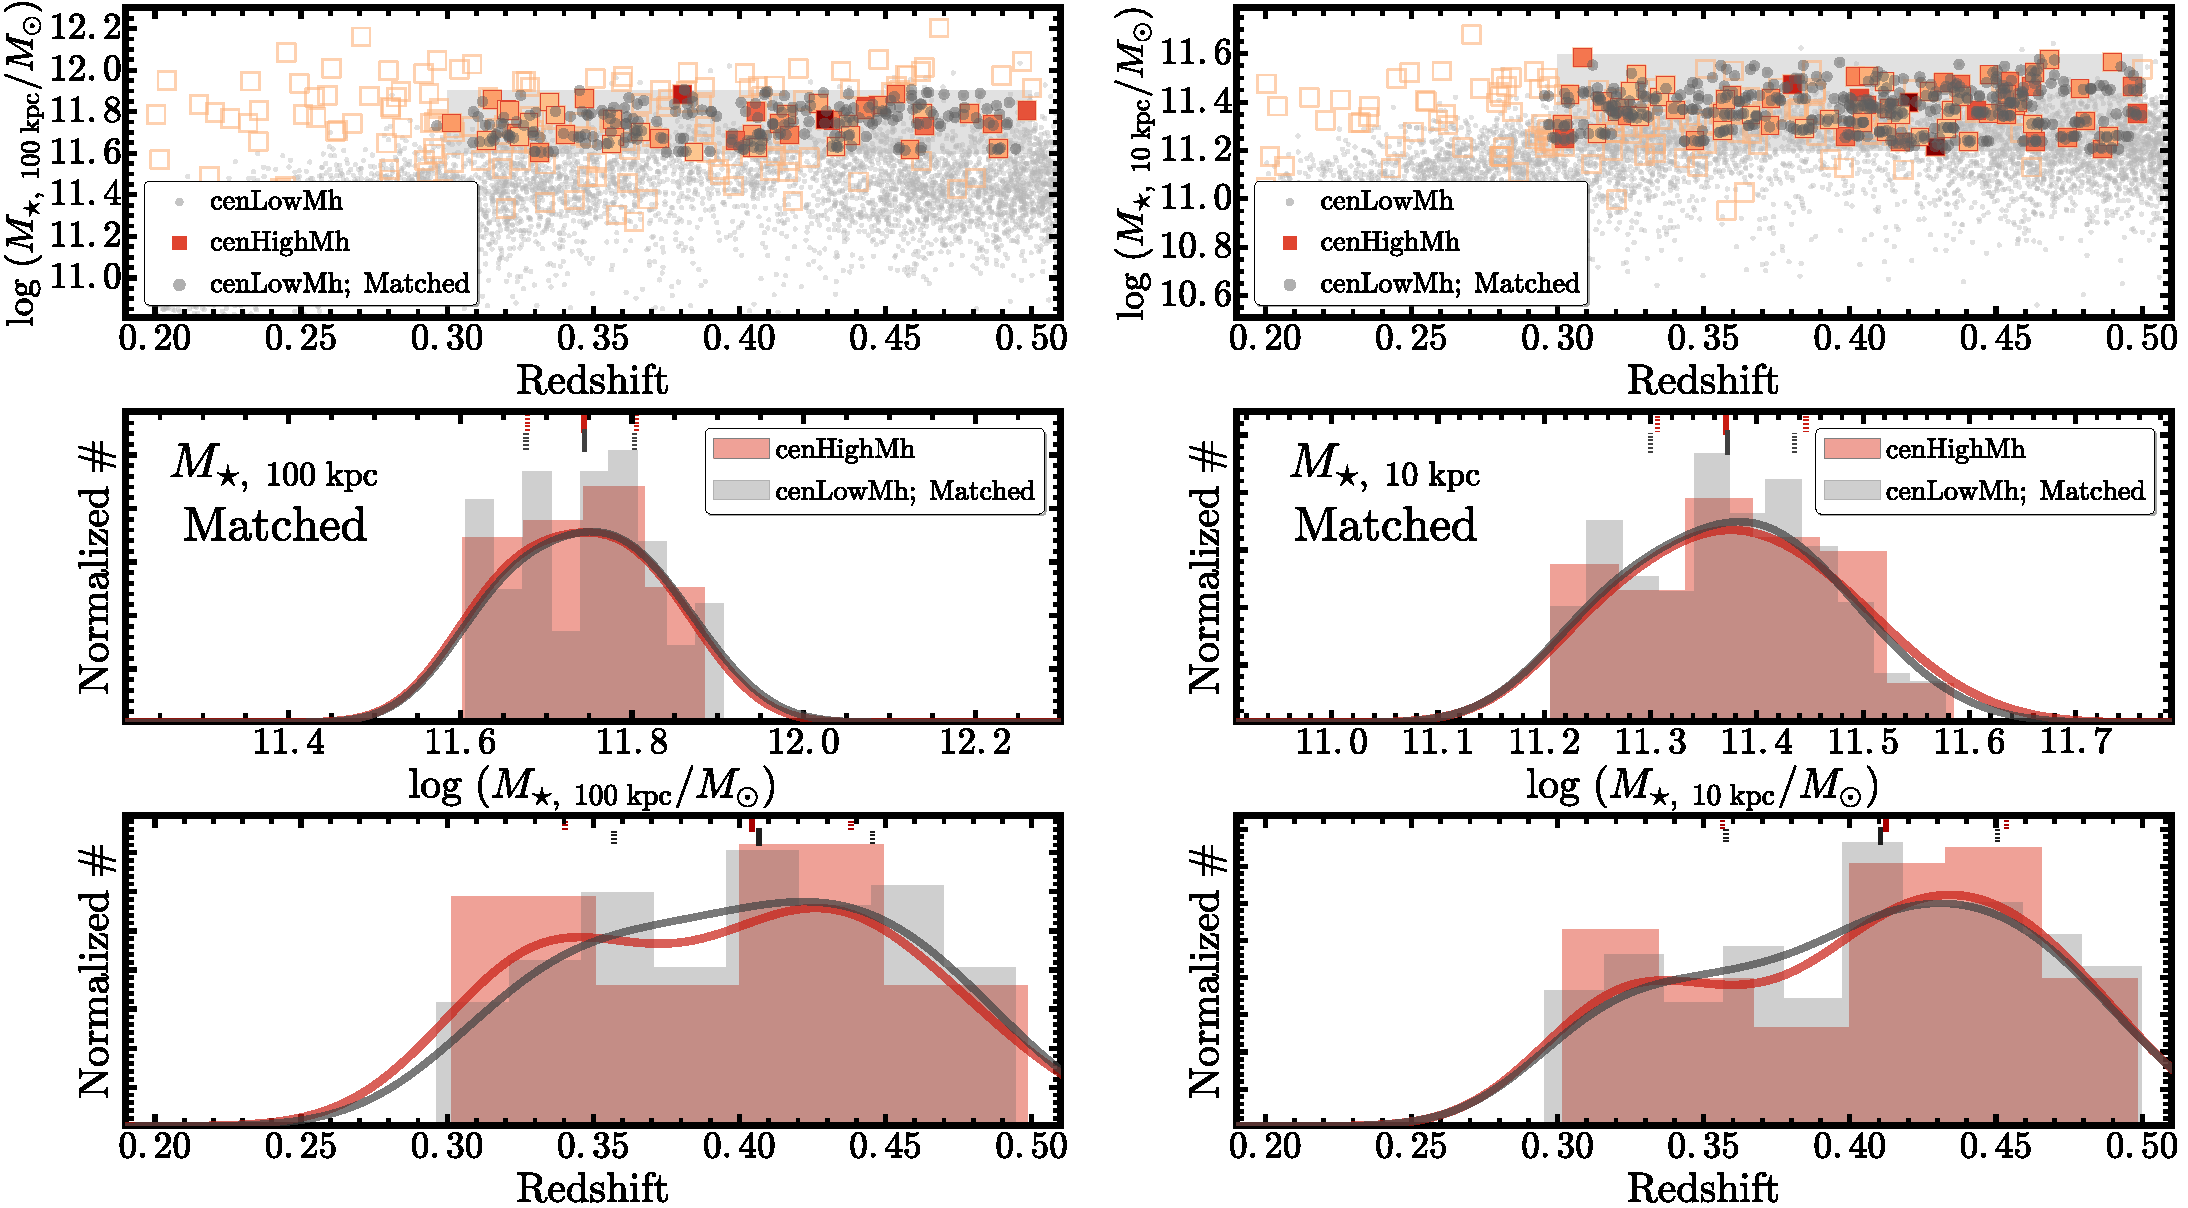
\includegraphics[width=\textwidth]{fig/redbcg_match}
    \caption{\textbf{Left figure} shows the details of the \mtot{}-matching process, 
        corresponding to the results shown in the left figure of   
        On the top panel, we show the overall distributions of \rbcg{} (light orange boxes) 
        and \nbcg{} (light grey dots) galaxies on the \mtot{}-$z$ plane.  
        And, we match the two sample in the \mtot{}-$z$ space outlined by the shaded region.
        We highlight the \rbcg{} galaxies in this region using bigger boxes in red frames, 
        whose size reflects the $P_{\mathrm{Cen}}$ value.  
        We also color-code them using the richness ($\lambda$) of the host cluster. 
        The matched \nbcg{} galaxies are highlighted using darker color and bigger dots. 
        To further evaluate the matching results, we show the distributions of \mtot{} 
        (middle panel) and redshift (bottom panel) separately. 
        On both panesl, we show the histograms along with their kernel density 
        distributions.  
        And, on the top of each panel, two sets of short vertical lines highlight the median 
        value (solid) and the inter-quartile (dash) of each distribution.~~~
        \textbf{Right figure} shows the similar matching results for the \minn{}-matched
        samples used for the right figure of Fig.\ref{fig:prof_1}.
        The format is exactly the same as the left one, except the \minn{} replaces the 
        \mtot{} in the top and middle panels.}
    \label{fig:match}
\end{figure*}
%% ------------------------------------------------------------------------------------ %% 
    
    \song{Still need some adjustments}
    
    As stellar mass is considered the most important parameter in determining the 
    structure and other properties of massive galaxies, it is crucial to make sure 
    the comparison is conducted at ``fixed stellar mass''. 
    And, since we directly compare the stellar mass distributions across very large 
    range in radius, it is also important to make sure that differences in physical 
    size of PSF (for more discussion on this issue, please see Appendix.\ref{app:C}) 
    and imaging depth do not affect the result.    
    In practice, we achieve these by matching the \rbcg{} and \nbcg{} samples in 
    the distributions of \mstar{} and redshift in the mass range where both 
    samples have decent completeness.  
    Since the \rbcg{} sample is much smaller in size, we match the \nbcg{} sample to it 
    by searching for the $N$ nearest neighbours on the $M_{\star}$-redshift 
    plane using the KDTree algorithm provided by \texttt{scikit-learn} Python 
    library (\citealt{scikit-learn}). 
    The quality of the matched sample is evaluated by not just the median values 
    of stellar mass and redshift, but also the kernel density distributions (KDE) 
    of these two properties.
    For \mstar{}, we use a Gaussian kernel with width equals to the typical 
    uncertainty of the mass estimate (0.06-0.10);
    and for redshift, we choose 0.025 as the width of the Gaussian kernel. 
    As we only keep unique \nbcg{} galaxies in the matched sample, we manually adjust 
    the value of $N$ to achieve the most similar distribution. 
    In case that the distribution of stellar mass or redshift for \rbcg{} is 
    bi-model, we also try to split the sample into two, and match them separately.
    Normally $N$ is between 3 to 8.
    
    \mstar{} within different radius traces different physical processes and 
    different epochs in the assembly history.  
    In this section, we match the two samples using our proxy of ``total'' stellar 
    mass, which is the \mstar{} within 100 kpc radius.  
    This choice reflects the stellar mass distributions we can safely measure using 
    model-independent approach given the current depth of the image and the accuracy 
    of sky background subtraction.
    For galaxies at $11.6 \leq \log(M_{\star}/M_{\odot}) < 11.9$, 100 kpc equals to 
    5-8 times of their effective radius, hence should enclose most their stellar mass.
    Also, for a fraction of massive \rbcg{} galaxies, the intra-group/cluster light
    (IGL/ICL) could dominate their mass profiles outside 100 kpc (\addref), and 
    complicate the comparison with the \nbcg{} galaxies.  
    We will discuss these issues later in Section \ref{sec:discussion}, but in 
    conclusion, the proxy of total \mstar{} and the potential ICL component should 
    not affect the results.     
    
    
\section{G. Robustness of the \mden{} Differences} 
	\label{app:robust}
    
    \song{Need some text!}
 
%% ------------------------------------------------------------------------------------ %% 
  \begin{figure*}[t!]
      \centering 
      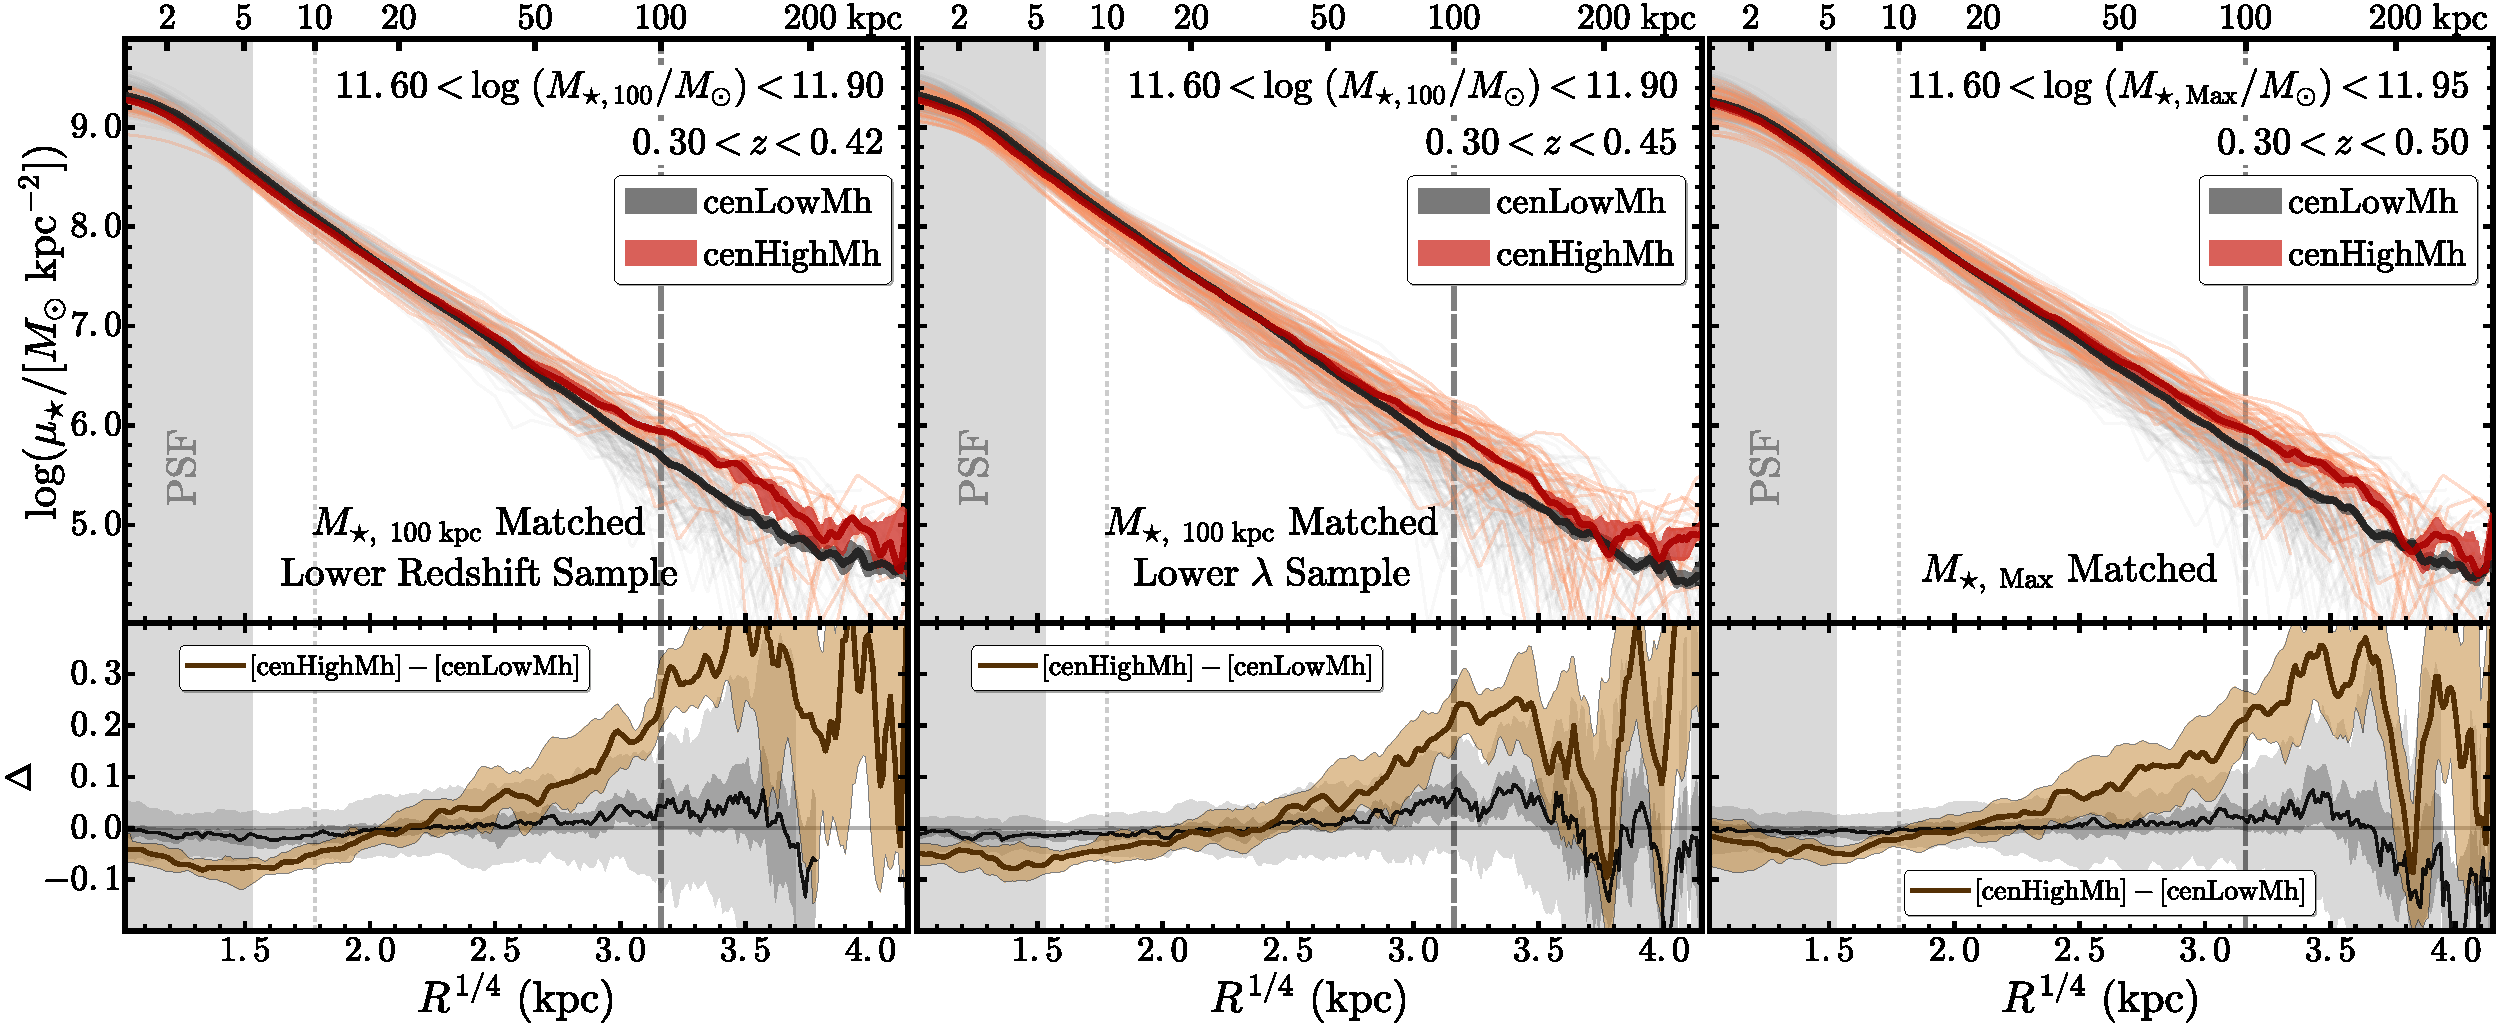
\includegraphics[width=\textwidth]{fig/redbcg_prof_3}
      \caption{Comparisons of the \mden{} profiles for \rbcg{} (orange-red) and \nbcg{} 
      	(grey-black) galaxies that are matched using proxies of total \mstar{}. 
        The formats are in consistent with the right figure of Fig.\ref{fig:prof_1}.
        The differences are, here, the samples are matched in slightly differnt ways. 
        From left to right: a) using samples at lower redshift ($0.3 < z < 0.4$); 
        b) using \rbcg{} sample with $\lambda > 20$ instead of 30; 
        c) using \mstar{} within 150 kpc instead of 100 kpc.
        The results are broadly consistent with the one in Fig.\ref{fig:prof_1}.}
      \label{fig:prof_3} 
  \end{figure*}
%% ------------------------------------------------------------------------------------ %% 

%% ------------------------------------------------------------------------------------ %% 
  \begin{figure*}[t!]
      \centering 
      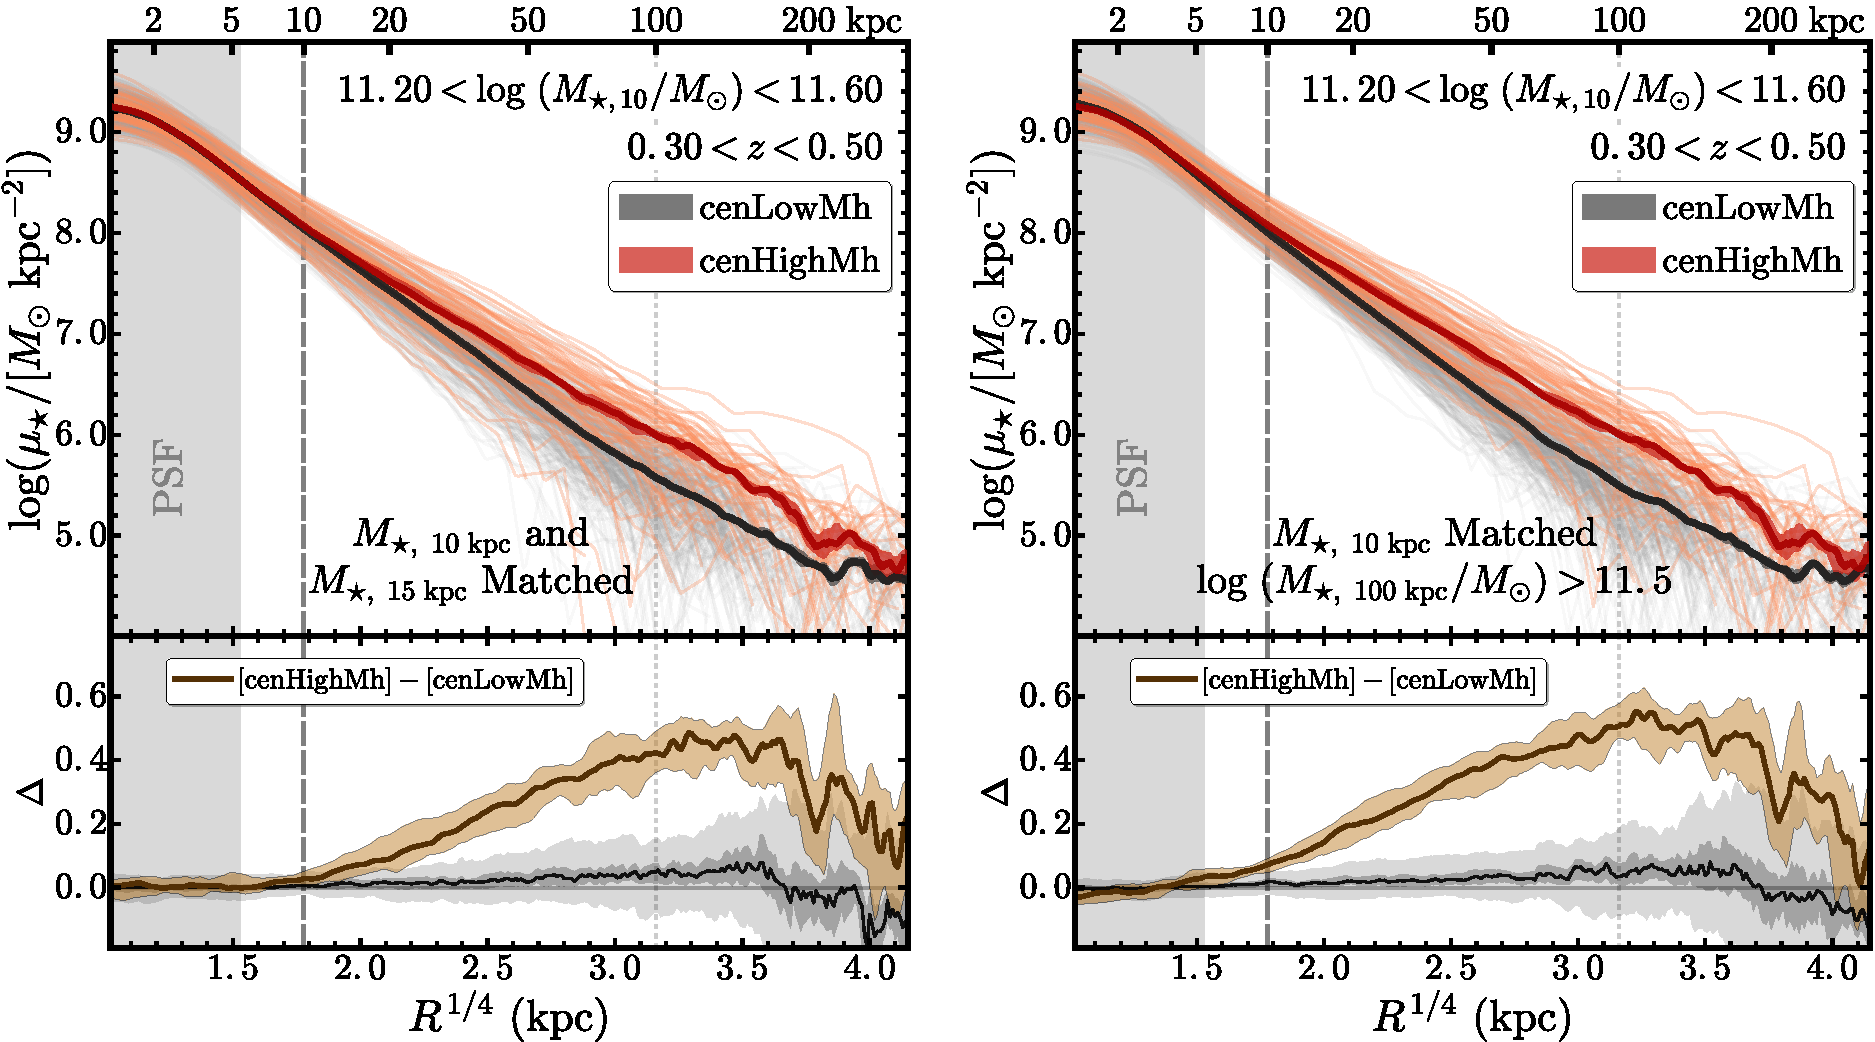
\includegraphics[width=\textwidth]{fig/redbcg_prof_4}
      \caption{Comparisons of the \mden{} profiles for \rbcg{} (orange-red) and \nbcg{} 
          (grey-black) galaxies that are matched using the \mstar{} enclosed in the 
          inner region. 
          Left panel shows the results after matching the \minn{} and \meff{} together, 
          and the right panel shows the results when only the \logmtot{}$\ge 11.5$
          \rbcg{} and \nbcg{} galaxies are included.
          Other formats are in consistent with the right figure of Fig.\ref{fig:prof_1}.}
      \label{fig:prof_4} 
  \end{figure*}
%% ------------------------------------------------------------------------------------ %% 
     
%% ------------------------------------------------------------------------------------ %% 
%% Table.1 
%% ------------------------------------------------------------------------------------ %% 
\clearpage
\begin{deluxetable}{c ccc cc cc}[b!]
\tabletypesize{\scriptsize}
\tablewidth{0pt}
\tablecolumns{8}
\tablenum{1}
\tablecaption{Average \mden{} Profiles of Massive Galaxies in Different Stellar Mass Bins}
%% ------------------------------------------------------------------------------------ %% 
\tablehead{
    \colhead{Radius} & 
    \multicolumn{3}{c}{[\mden{}]; Combined samples} &
    \multicolumn{2}{c}{[\mden{}]; $M_{\star,100\ \mathrm{kpc}}$-matched} &
    \multicolumn{2}{c}{[\mden{}]; $M_{\star,10\ \mathrm{kpc}}$-matched}
	\vspace{1.4ex}
    %------------------------------------------------------------------------------------%
    \nl 
    \colhead{kpc} & 
    \multicolumn{3}{c}{$\log (M_{\odot}/\mathrm{kpc}^2)$} &
    \multicolumn{2}{c}{$\log (M_{\odot}/\mathrm{kpc}^2)$} &
    \multicolumn{2}{c}{$\log (M_{\odot}/\mathrm{kpc}^2)$}
	\vspace{1.4ex}
    %------------------------------------------------------------------------------------%
    \nl 
    \colhead{} & 
    \colhead{$\log \frac{M_{\star,100\mathrm{kpc}}}{M_{\odot}}\in$[11.4, 11.6]} & 
    \colhead{[11.6, 11.8]} & 
    \colhead{[11.8, 12.0]}\hspace{2.0ex} & 
    \colhead{\texttt{cenHighMh}} & 
    \colhead{\texttt{cenLowMh}} & 
    \colhead{\texttt{cenHighMh}}\hspace{2.0ex} & 
    \colhead{\texttt{cenLowMh}}
    %------------------------------------------------------------------------------------%
	\vspace{1.6ex}
    %------------------------------------------------------------------------------------%
    \nl
    \colhead{    (1)} &
    \colhead{    (2)} &
    \colhead{    (3)} &
    \colhead{    (4)} &
    \colhead{    (5)} &
    \colhead{    (6)} &
    \colhead{    (7)} &
    \colhead{    (8)}
    %------------------------------------------------------------------------------------%
}
%% ------------------------------------------------------------------------------------ %% 
\startdata
%% ------------------------------------------------------------------------------------ %% 

0.0 & $ 9.23\substack{+0.00 \\ -0.00}$ &$ 9.31\substack{+0.00 \\ -0.01}$ &$ 9.32\substack{+0.01 \\ -0.01}$ &$ 9.31\substack{+0.02 \\ -0.02}$ &$ 9.34\substack{+0.01 \\ -0.01}$ &$ 9.31\substack{+0.02 \\ -0.02}$ &$ 9.34\substack{+0.02 \\ -0.02}$ \\
 0.6 & $ 9.20\substack{+0.00 \\ -0.00}$ &$ 9.28\substack{+0.00 \\ -0.01}$ &$ 9.29\substack{+0.01 \\ -0.01}$ &$ 9.27\substack{+0.02 \\ -0.02}$ &$ 9.31\substack{+0.01 \\ -0.01}$ &$ 9.28\substack{+0.02 \\ -0.02}$ &$ 9.31\substack{+0.02 \\ -0.02}$ \\
 1.0 & $ 9.16\substack{+0.00 \\ -0.00}$ &$ 9.24\substack{+0.00 \\ -0.00}$ &$ 9.26\substack{+0.01 \\ -0.01}$ &$ 9.24\substack{+0.02 \\ -0.02}$ &$ 9.27\substack{+0.01 \\ -0.01}$ &$ 9.25\substack{+0.02 \\ -0.02}$ &$ 9.27\substack{+0.02 \\ -0.02}$ \\
 1.4 & $ 9.12\substack{+0.00 \\ -0.00}$ &$ 9.20\substack{+0.00 \\ -0.00}$ &$ 9.23\substack{+0.01 \\ -0.01}$ &$ 9.20\substack{+0.02 \\ -0.02}$ &$ 9.23\substack{+0.01 \\ -0.01}$ &$ 9.21\substack{+0.02 \\ -0.01}$ &$ 9.23\substack{+0.02 \\ -0.01}$ \\
 1.7 & $ 9.06\substack{+0.00 \\ -0.00}$ &$ 9.15\substack{+0.00 \\ -0.00}$ &$ 9.19\substack{+0.01 \\ -0.01}$ &$ 9.15\substack{+0.02 \\ -0.02}$ &$ 9.19\substack{+0.01 \\ -0.01}$ &$ 9.16\substack{+0.01 \\ -0.01}$ &$ 9.18\substack{+0.01 \\ -0.01}$ \\
 2.0 & $ 9.00\substack{+0.00 \\ -0.00}$ &$ 9.10\substack{+0.00 \\ -0.00}$ &$ 9.15\substack{+0.01 \\ -0.01}$ &$ 9.09\substack{+0.01 \\ -0.02}$ &$ 9.13\substack{+0.01 \\ -0.01}$ &$ 9.11\substack{+0.01 \\ -0.01}$ &$ 9.12\substack{+0.01 \\ -0.01}$ \\
 2.4 & $ 8.93\substack{+0.00 \\ -0.00}$ &$ 9.03\substack{+0.00 \\ -0.00}$ &$ 9.09\substack{+0.01 \\ -0.01}$ &$ 9.03\substack{+0.02 \\ -0.02}$ &$ 9.07\substack{+0.01 \\ -0.01}$ &$ 9.05\substack{+0.01 \\ -0.01}$ &$ 9.05\substack{+0.01 \\ -0.01}$ \\
 2.7 & $ 8.87\substack{+0.00 \\ -0.00}$ &$ 8.97\substack{+0.00 \\ -0.00}$ &$ 9.04\substack{+0.01 \\ -0.01}$ &$ 8.97\substack{+0.01 \\ -0.01}$ &$ 9.01\substack{+0.01 \\ -0.01}$ &$ 9.00\substack{+0.01 \\ -0.01}$ &$ 8.99\substack{+0.01 \\ -0.01}$ \\
 3.0 & $ 8.80\substack{+0.00 \\ -0.00}$ &$ 8.90\substack{+0.00 \\ -0.00}$ &$ 8.98\substack{+0.01 \\ -0.01}$ &$ 8.90\substack{+0.01 \\ -0.01}$ &$ 8.95\substack{+0.01 \\ -0.01}$ &$ 8.93\substack{+0.01 \\ -0.01}$ &$ 8.92\substack{+0.01 \\ -0.01}$ \\
 3.4 & $ 8.72\substack{+0.00 \\ -0.00}$ &$ 8.83\substack{+0.00 \\ -0.00}$ &$ 8.92\substack{+0.01 \\ -0.01}$ &$ 8.83\substack{+0.01 \\ -0.01}$ &$ 8.88\substack{+0.01 \\ -0.01}$ &$ 8.86\substack{+0.01 \\ -0.01}$ &$ 8.85\substack{+0.01 \\ -0.01}$ \\
 3.7 & $ 8.66\substack{+0.00 \\ -0.00}$ &$ 8.78\substack{+0.00 \\ -0.00}$ &$ 8.87\substack{+0.01 \\ -0.01}$ &$ 8.78\substack{+0.01 \\ -0.01}$ &$ 8.83\substack{+0.01 \\ -0.01}$ &$ 8.81\substack{+0.01 \\ -0.01}$ &$ 8.79\substack{+0.01 \\ -0.01}$ \\
 4.1 & $ 8.60\substack{+0.00 \\ -0.00}$ &$ 8.72\substack{+0.00 \\ -0.00}$ &$ 8.82\substack{+0.01 \\ -0.01}$ &$ 8.72\substack{+0.01 \\ -0.01}$ &$ 8.77\substack{+0.01 \\ -0.01}$ &$ 8.76\substack{+0.01 \\ -0.01}$ &$ 8.73\substack{+0.01 \\ -0.01}$ \\
 4.4 & $ 8.54\substack{+0.00 \\ -0.00}$ &$ 8.66\substack{+0.00 \\ -0.00}$ &$ 8.77\substack{+0.01 \\ -0.01}$ &$ 8.66\substack{+0.01 \\ -0.01}$ &$ 8.72\substack{+0.01 \\ -0.01}$ &$ 8.70\substack{+0.01 \\ -0.01}$ &$ 8.67\substack{+0.01 \\ -0.01}$ \\
 4.8 & $ 8.48\substack{+0.00 \\ -0.00}$ &$ 8.60\substack{+0.00 \\ -0.00}$ &$ 8.71\substack{+0.01 \\ -0.01}$ &$ 8.60\substack{+0.01 \\ -0.01}$ &$ 8.66\substack{+0.01 \\ -0.01}$ &$ 8.65\substack{+0.01 \\ -0.01}$ &$ 8.61\substack{+0.01 \\ -0.01}$ \\
 6.2 & $ 8.26\substack{+0.00 \\ -0.00}$ &$ 8.40\substack{+0.00 \\ -0.00}$ &$ 8.53\substack{+0.01 \\ -0.01}$ &$ 8.41\substack{+0.01 \\ -0.01}$ &$ 8.46\substack{+0.01 \\ -0.01}$ &$ 8.46\substack{+0.02 \\ -0.02}$ &$ 8.40\substack{+0.02 \\ -0.02}$ \\
 7.6 & $ 8.09\substack{+0.00 \\ -0.00}$ &$ 8.24\substack{+0.00 \\ -0.00}$ &$ 8.39\substack{+0.01 \\ -0.01}$ &$ 8.27\substack{+0.01 \\ -0.01}$ &$ 8.31\substack{+0.01 \\ -0.01}$ &$ 8.31\substack{+0.02 \\ -0.02}$ &$ 8.23\substack{+0.02 \\ -0.02}$ \\
 9.0 & $ 7.95\substack{+0.00 \\ -0.00}$ &$ 8.10\substack{+0.00 \\ -0.00}$ &$ 8.27\substack{+0.01 \\ -0.01}$ &$ 8.14\substack{+0.02 \\ -0.02}$ &$ 8.18\substack{+0.01 \\ -0.01}$ &$ 8.19\substack{+0.02 \\ -0.02}$ &$ 8.09\substack{+0.02 \\ -0.02}$ \\
10.3 & $ 7.82\substack{+0.00 \\ -0.00}$ &$ 7.99\substack{+0.00 \\ -0.00}$ &$ 8.16\substack{+0.01 \\ -0.01}$ &$ 8.03\substack{+0.02 \\ -0.01}$ &$ 8.06\substack{+0.01 \\ -0.01}$ &$ 8.09\substack{+0.02 \\ -0.02}$ &$ 7.97\substack{+0.02 \\ -0.02}$ \\
11.7 & $ 7.70\substack{+0.00 \\ -0.00}$ &$ 7.88\substack{+0.00 \\ -0.00}$ &$ 8.06\substack{+0.01 \\ -0.01}$ &$ 7.93\substack{+0.02 \\ -0.02}$ &$ 7.96\substack{+0.01 \\ -0.01}$ &$ 7.99\substack{+0.02 \\ -0.02}$ &$ 7.85\substack{+0.02 \\ -0.02}$ \\
13.0 & $ 7.60\substack{+0.00 \\ -0.00}$ &$ 7.78\substack{+0.00 \\ -0.00}$ &$ 7.98\substack{+0.01 \\ -0.01}$ &$ 7.85\substack{+0.02 \\ -0.02}$ &$ 7.87\substack{+0.01 \\ -0.01}$ &$ 7.90\substack{+0.02 \\ -0.02}$ &$ 7.75\substack{+0.02 \\ -0.02}$ \\
14.5 & $ 7.50\substack{+0.00 \\ -0.00}$ &$ 7.69\substack{+0.00 \\ -0.00}$ &$ 7.90\substack{+0.01 \\ -0.01}$ &$ 7.76\substack{+0.02 \\ -0.02}$ &$ 7.78\substack{+0.01 \\ -0.01}$ &$ 7.82\substack{+0.02 \\ -0.02}$ &$ 7.65\substack{+0.02 \\ -0.02}$ \\
16.0 & $ 7.39\substack{+0.00 \\ -0.00}$ &$ 7.60\substack{+0.00 \\ -0.00}$ &$ 7.82\substack{+0.01 \\ -0.01}$ &$ 7.68\substack{+0.02 \\ -0.02}$ &$ 7.69\substack{+0.01 \\ -0.01}$ &$ 7.74\substack{+0.02 \\ -0.03}$ &$ 7.56\substack{+0.02 \\ -0.03}$ \\
17.3 & $ 7.31\substack{+0.00 \\ -0.00}$ &$ 7.52\substack{+0.00 \\ -0.00}$ &$ 7.76\substack{+0.01 \\ -0.01}$ &$ 7.61\substack{+0.02 \\ -0.02}$ &$ 7.62\substack{+0.01 \\ -0.01}$ &$ 7.67\substack{+0.03 \\ -0.03}$ &$ 7.48\substack{+0.03 \\ -0.03}$ \\
18.7 & $ 7.23\substack{+0.00 \\ -0.00}$ &$ 7.45\substack{+0.00 \\ -0.00}$ &$ 7.69\substack{+0.01 \\ -0.01}$ &$ 7.55\substack{+0.02 \\ -0.02}$ &$ 7.55\substack{+0.01 \\ -0.01}$ &$ 7.61\substack{+0.03 \\ -0.03}$ &$ 7.40\substack{+0.03 \\ -0.03}$ \\
22.6 & $ 7.02\substack{+0.00 \\ -0.00}$ &$ 7.27\substack{+0.00 \\ -0.00}$ &$ 7.54\substack{+0.01 \\ -0.01}$ &$ 7.38\substack{+0.02 \\ -0.02}$ &$ 7.37\substack{+0.01 \\ -0.01}$ &$ 7.45\substack{+0.03 \\ -0.03}$ &$ 7.21\substack{+0.03 \\ -0.03}$ \\
26.1 & $ 6.86\substack{+0.00 \\ -0.00}$ &$ 7.12\substack{+0.00 \\ -0.00}$ &$ 7.41\substack{+0.01 \\ -0.01}$ &$ 7.25\substack{+0.02 \\ -0.02}$ &$ 7.24\substack{+0.01 \\ -0.01}$ &$ 7.32\substack{+0.03 \\ -0.03}$ &$ 7.05\substack{+0.03 \\ -0.03}$ \\
30.0 & $ 6.70\substack{+0.00 \\ -0.00}$ &$ 6.98\substack{+0.00 \\ -0.00}$ &$ 7.29\substack{+0.01 \\ -0.01}$ &$ 7.13\substack{+0.03 \\ -0.02}$ &$ 7.10\substack{+0.01 \\ -0.01}$ &$ 7.20\substack{+0.03 \\ -0.04}$ &$ 6.90\substack{+0.03 \\ -0.04}$ \\
33.7 & $ 6.55\substack{+0.00 \\ -0.00}$ &$ 6.85\substack{+0.01 \\ -0.01}$ &$ 7.18\substack{+0.01 \\ -0.01}$ &$ 7.01\substack{+0.03 \\ -0.03}$ &$ 6.98\substack{+0.01 \\ -0.01}$ &$ 7.09\substack{+0.03 \\ -0.03}$ &$ 6.76\substack{+0.03 \\ -0.03}$ \\
37.8 & $ 6.41\substack{+0.00 \\ -0.00}$ &$ 6.72\substack{+0.01 \\ -0.01}$ &$ 7.07\substack{+0.01 \\ -0.01}$ &$ 6.90\substack{+0.03 \\ -0.03}$ &$ 6.85\substack{+0.01 \\ -0.01}$ &$ 6.98\substack{+0.04 \\ -0.04}$ &$ 6.63\substack{+0.04 \\ -0.04}$ \\
41.6 & $ 6.29\substack{+0.01 \\ -0.01}$ &$ 6.61\substack{+0.01 \\ -0.01}$ &$ 6.98\substack{+0.01 \\ -0.01}$ &$ 6.81\substack{+0.03 \\ -0.03}$ &$ 6.75\substack{+0.01 \\ -0.01}$ &$ 6.89\substack{+0.04 \\ -0.04}$ &$ 6.51\substack{+0.04 \\ -0.04}$ \\
45.7 & $ 6.17\substack{+0.01 \\ -0.01}$ &$ 6.50\substack{+0.01 \\ -0.01}$ &$ 6.88\substack{+0.01 \\ -0.01}$ &$ 6.71\substack{+0.03 \\ -0.03}$ &$ 6.64\substack{+0.01 \\ -0.01}$ &$ 6.79\substack{+0.04 \\ -0.04}$ &$ 6.39\substack{+0.04 \\ -0.04}$ \\
49.3 & $ 6.07\substack{+0.01 \\ -0.01}$ &$ 6.41\substack{+0.01 \\ -0.01}$ &$ 6.80\substack{+0.01 \\ -0.02}$ &$ 6.62\substack{+0.03 \\ -0.03}$ &$ 6.56\substack{+0.01 \\ -0.01}$ &$ 6.70\substack{+0.04 \\ -0.04}$ &$ 6.30\substack{+0.04 \\ -0.04}$ \\
53.1 & $ 5.98\substack{+0.01 \\ -0.01}$ &$ 6.33\substack{+0.01 \\ -0.01}$ &$ 6.71\substack{+0.02 \\ -0.02}$ &$ 6.55\substack{+0.03 \\ -0.03}$ &$ 6.46\substack{+0.01 \\ -0.01}$ &$ 6.64\substack{+0.04 \\ -0.04}$ &$ 6.21\substack{+0.04 \\ -0.04}$ \\
57.2 & $ 5.88\substack{+0.01 \\ -0.01}$ &$ 6.24\substack{+0.01 \\ -0.01}$ &$ 6.63\substack{+0.02 \\ -0.02}$ &$ 6.47\substack{+0.04 \\ -0.04}$ &$ 6.37\substack{+0.01 \\ -0.01}$ &$ 6.56\substack{+0.04 \\ -0.04}$ &$ 6.11\substack{+0.04 \\ -0.04}$ \\
61.5 & $ 5.79\substack{+0.01 \\ -0.01}$ &$ 6.15\substack{+0.01 \\ -0.01}$ &$ 6.55\substack{+0.02 \\ -0.02}$ &$ 6.39\substack{+0.04 \\ -0.04}$ &$ 6.29\substack{+0.01 \\ -0.01}$ &$ 6.49\substack{+0.04 \\ -0.04}$ &$ 6.03\substack{+0.04 \\ -0.04}$ \\
66.0 & $ 5.70\substack{+0.01 \\ -0.01}$ &$ 6.05\substack{+0.01 \\ -0.01}$ &$ 6.47\substack{+0.02 \\ -0.02}$ &$ 6.32\substack{+0.04 \\ -0.04}$ &$ 6.20\substack{+0.01 \\ -0.01}$ &$ 6.37\substack{+0.05 \\ -0.06}$ &$ 5.94\substack{+0.05 \\ -0.06}$ \\
69.8 & $ 5.64\substack{+0.01 \\ -0.01}$ &$ 5.98\substack{+0.01 \\ -0.01}$ &$ 6.40\substack{+0.02 \\ -0.02}$ &$ 6.25\substack{+0.04 \\ -0.04}$ &$ 6.12\substack{+0.02 \\ -0.01}$ &$ 6.35\substack{+0.04 \\ -0.05}$ &$ 5.87\substack{+0.04 \\ -0.05}$ \\
74.7 & $ 5.56\substack{+0.01 \\ -0.01}$ &$ 5.89\substack{+0.01 \\ -0.01}$ &$ 6.32\substack{+0.02 \\ -0.02}$ &$ 6.18\substack{+0.04 \\ -0.04}$ &$ 6.04\substack{+0.02 \\ -0.02}$ &$ 6.28\substack{+0.05 \\ -0.05}$ &$ 5.79\substack{+0.05 \\ -0.05}$ \\
79.9 & $ 5.49\substack{+0.01 \\ -0.01}$ &$ 5.81\substack{+0.01 \\ -0.01}$ &$ 6.24\substack{+0.02 \\ -0.02}$ &$ 6.12\substack{+0.04 \\ -0.04}$ &$ 5.96\substack{+0.02 \\ -0.02}$ &$ 6.20\substack{+0.05 \\ -0.06}$ &$ 5.72\substack{+0.05 \\ -0.06}$ \\
84.3 & $ 5.43\substack{+0.01 \\ -0.01}$ &$ 5.74\substack{+0.01 \\ -0.01}$ &$ 6.18\substack{+0.02 \\ -0.02}$ &$ 6.05\substack{+0.04 \\ -0.05}$ &$ 5.89\substack{+0.02 \\ -0.02}$ &$ 6.16\substack{+0.05 \\ -0.05}$ &$ 5.65\substack{+0.05 \\ -0.05}$ \\
88.8 & $ 5.38\substack{+0.01 \\ -0.01}$ &$ 5.67\substack{+0.01 \\ -0.01}$ &$ 6.11\substack{+0.02 \\ -0.02}$ &$ 5.99\substack{+0.05 \\ -0.06}$ &$ 5.81\substack{+0.02 \\ -0.02}$ &$ 6.08\substack{+0.05 \\ -0.06}$ &$ 5.58\substack{+0.05 \\ -0.06}$ \\
97.2 & $ 5.29\substack{+0.01 \\ -0.01}$ &$ 5.56\substack{+0.01 \\ -0.01}$ &$ 5.98\substack{+0.02 \\ -0.02}$ &$ 5.92\substack{+0.04 \\ -0.04}$ &$ 5.69\substack{+0.02 \\ -0.02}$ &$ 5.99\substack{+0.05 \\ -0.05}$ &$ 5.47\substack{+0.05 \\ -0.05}$ \\
103.6 & $ 5.21\substack{+0.01 \\ -0.01}$ &$ 5.49\substack{+0.01 \\ -0.01}$ &$ 5.89\substack{+0.03 \\ -0.03}$ &$ 5.84\substack{+0.05 \\ -0.05}$ &$ 5.62\substack{+0.02 \\ -0.02}$ &$ 5.94\substack{+0.05 \\ -0.05}$ &$ 5.39\substack{+0.05 \\ -0.05}$ \\
111.6 & $ 5.14\substack{+0.01 \\ -0.01}$ &$ 5.40\substack{+0.01 \\ -0.01}$ &$ 5.79\substack{+0.03 \\ -0.03}$ &$ 5.78\substack{+0.05 \\ -0.05}$ &$ 5.54\substack{+0.02 \\ -0.02}$ &$ 5.87\substack{+0.05 \\ -0.05}$ &$ 5.32\substack{+0.05 \\ -0.05}$ \\
117.2 & $ 5.10\substack{+0.01 \\ -0.01}$ &$ 5.36\substack{+0.01 \\ -0.01}$ &$ 5.72\substack{+0.03 \\ -0.03}$ &$ 5.72\substack{+0.05 \\ -0.05}$ &$ 5.47\substack{+0.02 \\ -0.02}$ &$ 5.82\substack{+0.05 \\ -0.05}$ &$ 5.29\substack{+0.05 \\ -0.05}$ \\
129.0 & $ 5.00\substack{+0.01 \\ -0.01}$ &$ 5.25\substack{+0.02 \\ -0.02}$ &$ 5.61\substack{+0.03 \\ -0.03}$ &$ 5.64\substack{+0.05 \\ -0.05}$ &$ 5.36\substack{+0.02 \\ -0.02}$ &$ 5.74\substack{+0.05 \\ -0.05}$ &$ 5.21\substack{+0.05 \\ -0.05}$ \\
141.7 & $ 4.89\substack{+0.02 \\ -0.02}$ &$ 5.13\substack{+0.02 \\ -0.02}$ &$ 5.49\substack{+0.03 \\ -0.03}$ &$ 5.58\substack{+0.05 \\ -0.05}$ &$ 5.23\substack{+0.03 \\ -0.03}$ &$ 5.66\substack{+0.05 \\ -0.05}$ &$ 5.09\substack{+0.05 \\ -0.05}$ \\
146.7 & $ 4.85\substack{+0.02 \\ -0.02}$ &$ 5.10\substack{+0.02 \\ -0.02}$ &$ 5.46\substack{+0.03 \\ -0.03}$ &$ 5.51\substack{+0.06 \\ -0.06}$ &$ 5.19\substack{+0.03 \\ -0.03}$ &$ 5.61\substack{+0.05 \\ -0.05}$ &$ 5.03\substack{+0.05 \\ -0.05}$ \\

%%------------------------------------------------------------------------------------ %% 
\enddata
%% ------------------------------------------------------------------------------------ %% 
\tablecomments{
    Average \mden{} profiles of massive \rbcg{} and \nbcg{} galaxies in different
    samples:\\ 
    Col.~(1) Radius along the major axis in kpc.\\
    Col.~(2) Average \mden{} profile for galaxies with 
        $11.4 \leq$\logmtot$< 11.6$ in the combined samples of \rbcg{} and \nbcg{}
        galaxies. \\ 
    Col.~(3) Average \mden{} profile of combined samples in the mass bin of 
        $11.6 \leq$\logmtot$< 11.8$. \\ 
    Col.~(4) Average \mden{} profile of combined samples in the mass bin of 
        $11.8 \leq$\logmtot$< 12.0$. \\ 
    Col.~(5) and Col.~(6) are the average \mden{} profiles of \rbcg{} and \nbcg{} galaxies
        in the \mtot{}-matched samples within $11.6 \leq$\logmtot{}$< 11.9$. \\ 
    Col.~(7) and Col.~(8) are the average \mden{} profiles of \rbcg{} and \nbcg{} galaxies 
        in the \minn{}-matched samples within $11.2 \leq$\logmtot{}$< 11.6$. \\ 
    The upper and lower uncertainties of these average profiles vial bootstrap-resampling 
    method are also displayed.
}
\label{tab:prof}
\end{deluxetable}


%% ------------------------------------------------------------------------------------ %% 

%% ------------------------------------------------------------------------------------ %% 
%%%%%%%%%%%%: End of the File %%%%%%%%%%%%
%% ------------------------------------------------------------------------------------ %% 

\end{CJK*}

\clearpage 

\label{lastpage}

\end{document}
%% ------------------------------------------------------------------------------------ %% 
